   
\documentclass[12pt]{article}
\usepackage{latexsym}
\usepackage{amsmath,exscale,relsize}
\usepackage{setspace}
\usepackage{amsmath,amssymb}
\usepackage[dvips]{graphicx}
\usepackage{graphicx,color}
\usepackage{rotating}
\setlength{\oddsidemargin}{-.06in}
\setlength{\textwidth}{6.5in} 
\setlength{\textheight}{8.8in}
\setlength{\topmargin}{-0.35in}
         
%%%%%%%%%%%%%%%%%%%%%%%%%%%%%%%%
                   
\begin{document}

\begin{center}

      \vspace*{6mm}

              {\bf\large         Dynamic Testing of\\
                            Wholesale Power Market Designs:}

\bigskip
                 {\bf\large An Open-Source Agent-Based Framework%
\footnote{An abridged version of this study is forthcoming in \textit{Computational Economics\/}. This work has been supported in part by the National Science Foundation under Grant NSF-0527460.  We are grateful to Deddy Koesrindartoto for collaboration on earlier phases of this project, and to Daniel Kirschen, Chen-Ching Liu, James McCalley, Herman Quirmbach, Harold Salazar, and especially Anke Weidlich for helpful discussions on topics related to this project.}}

\vspace*{8mm}

        {\bf Junjie Sun and Leigh Tesfatsion%
\footnote{Corresponding author, tesfatsi@iastate.edu, http://www.econ.iastate.edu/tesfatsi/.}}\\
         {\bf Economics Department, Iowa State University, IA 50011-1070}\\
    
\medskip

   
\vspace*{3mm}     
                        {\bf ISU Economics Working Paper No.~06025}\\
                       {\bf http://www.econ.iastate.edu/tesfatsi/DynTestAMES.JSLT.pdf}\\
                           {\bf Last Revised: 10 July 2007}

\end{center}


\pagestyle{plain}

\setcounter{page}{1}

\begin{center}  \textbf{ABSTRACT}  \end{center}

\smallskip

\noindent
In April 2003 the U.S. Federal Energy Regulatory Commission proposed a complicated market design -- the \textit{Wholesale Power Market Platform (WPMP)} -- for common adoption by all U.S. wholesale power markets.  Versions of the WPMP have been implemented in New England, New York, the mid-Atlantic states, the Midwest, the Southwest, and California. Strong opposition to the WPMP persists among some industry stakeholders, however, due largely to a perceived lack of adequate performance testing. This study reports on the model development and open-source implementation (in Java) of a computational wholesale power market organized in accordance with core WPMP features and operating over a realistically rendered transmission grid.  The traders within this market model are strategic profit-seeking agents whose learning behaviors are based on data from human-subject experiments.  Our key experimental focus is the complex interplay among structural conditions, market protocols, and learning behaviors in relation to short-term and longer-term market performance.  Findings for a dynamic 5-node transmission grid test case are presented for concrete illustration.   


\bigskip
\noindent \textbf{Keywords:} Wholesale power market restructuring; Empirical input validation; Market design; Behavioral economics; Learning; Market power; Agent-based modeling; AMES wholesale power market framework; Java; RepastJ.

\medskip 
\noindent 
\textbf{JEL Codes:} L1; D8; L9; C6

\vfill
      
\pagebreak
                
\section{Introduction}

\smallskip

\noindent 
The meltdown in the restructured California wholesale power market in the summer of 2000 has shown what can happen when a poorly designed market mechanism is implemented without proper testing.  The California crisis is believed to have resulted in part from strategic behaviors encouraged by inappropriate market design features (Borenstein, 2002).  Following the California crisis, many energy researchers have eloquently argued the need to combine structural understanding with economic analysis of incentives in order to develop wholesale power market designs with good real-world performance characteristics; see, for example, Amin~(2004).  

In April 2003 the U.S. Federal Energy Regulatory Commission
proposed the \textit{Wholesale Power Market Platform (WPMP)\/} 
as a template for all U.S.\ wholesale power markets (FERC, 2003).  As detailed in Wilson (2002), this 
design entails an integrated rather than unbundled market form; it recommends the operation of wholesale power markets  
by Independent System Operators (ISOs) or Regional Transmission 
Organizations (RTOs) using locational marginal pricing
to price energy by the location of its injection into or withdrawal from 
the transmission grid.  Versions of this design have been implemented 
in New England (ISO-NE), New York (NYISO), 
the mid-Atlantic states (PJM), the Midwest (MISO), the Southwest (SPP), and
California (CAISO).  Joskow (2006, p.~6) reports that ISO/RTO-operated energy regions 
now include over $50\%$ of the generating capacity in the U.S.; see Figure~\ref{fig:RTORegions}.

%%%%%%%%%%%%%%%%%%%%%%%%%%%%%%%%%%%%%%%

\begin{figure}[h]
	\centering
		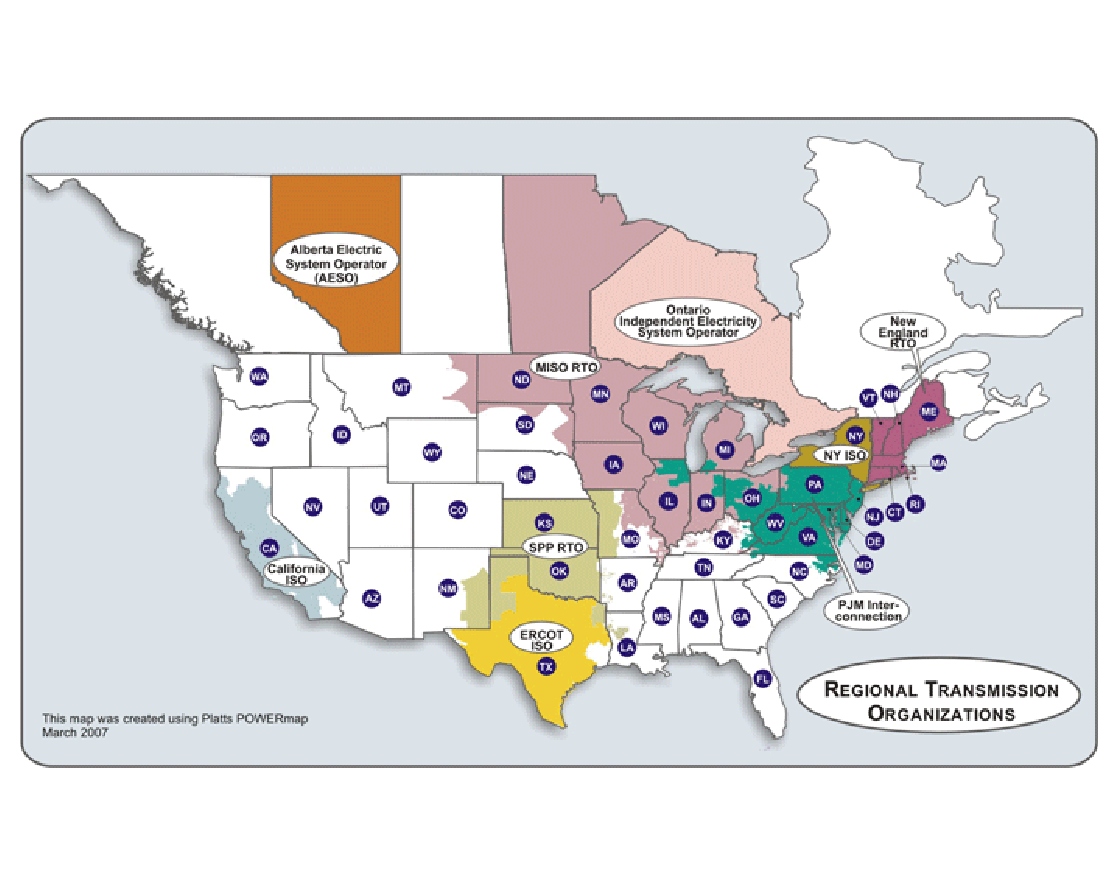
\includegraphics[totalheight = 10cm]{RTORegionsMar2007.eps}
	\caption{ISO/RTO-Operated U.S.\ Wholesale Power Markets 
(Source: FERC, http://www.ferc.gov/industries/electric/indus-act/rto/rto-map.asp)}
	\label{fig:RTORegions}
\end{figure}

%%%%%%%%%%%%%%%%%%%%%%%%%%%%%%%%%%%%%%%%%

The complexity of the WPMP market design
has made it extremely difficult to undertake economic and
physical reliability studies of the design using standard
statistical and analytical tools.  Strong opposition to the market design
thus persists among some industry stakeholders due in part to a
perceived lack of sufficient performance testing.

In recent years, however, powerful new agent-based computational tools have been developed 
to analyze this degree of complexity.   A variety of commercial agent-based frameworks are 
now available for the study of restructured electricity markets; see, for example, 
the EMCAS framework developed by researchers at the Argonne National Laboratory (Conzelmann et al., 2004).  
In addition, researchers such as Bower and Bunn (2001), Nicolaisen et al.~(2001), Veit et al.~(2006), and 
Widergren et al.~(2004) have used agent-based models to study important aspects of restructured electricity markets.%
    \footnote{See Tesfatsion (2007a) for extensive annotated pointers to agent-based electricity research.}

In a preliminary study (Koesrindartoto et al., 2005), we examined the feasibility and 
potential fruitfulness of \textit{Agent-based Computational Economics (ACE)\/} specifically for the study of the WPMP market design.  ACE is the computational study of economic processes modeled as dynamic systems of interacting agents.%
     \footnote{See Axelrod and Tesfatsion (2007), Tesfatsion (2007b), and Tesfatsion and Judd~(2006) for extensive introductory materials on ACE.}
       
Building on this prior work, the present study reports on the development and implementation of
an ACE framework for testing the dynamic efficiency and
reliability of the WPMP market design.  This framework 
-- referred to as {\it AMES\/} ({\it A\/}gent-based {\it
M\/}odeling of {\it E\/}lectricity {\it S\/}ystems) -- 
models strategic traders interacting over time in a wholesale power
market that is organized in accordance with core WPMP features
and that operates over a realistically rendered transmission
grid.  To our knowledge, AMES is the 
first non-commercial open-source framework permitting the 
computational study of the WPMP design.%
  \footnote{AMES can be obtained as free open-source software at Tesfatsion (2007c).}

To help ensure empirical input validity, the AMES framework has been developed by means of an 
iterative participatory modeling approach.%
  \footnote{See Barreteau (2003) for a fuller discussion of iterative participatory modeling, also called 
   \textit{companion modeling\/}.  For more general materials on empirical 
    validation methods for agent-based computational models, see Tesfatsion (2007d) and Windrum et al.~(2007).}
Specifically, we are engaging with industry participants and policy makers 
in an ongoing collaborative learning process involving four repeated stages 
of analysis: fieldwork and data collection;
scenario discussion and role-playing games; agent-based model development; and intensive
computational experiments.  We are relying heavily on
business practices from two adopters of the WPMP design (New
England and the Midwest) for our implementation of market
structure, market architecture, and dispatch and pricing
solutions.  We have also incorporated reinforcement learning representations
for the electricity traders that are based on findings from
human-subject multi-agent game experiments conducted by Roth and Erev (1995).%
   \footnote{Real-world market traders are understandably reluctant to discuss with us the precise manner in which they determine their supply offers and demand bids, so indirect identification methods must be used.} 

We are currently using the AMES framework 
to investigate the intermediate-term performance of wholesale power markets 
operating under the WPMP market design.  In particular, we are exploring the extent to which this design
is capable of supporting the efficient, profitable, and sustainable operation over time of existing generation and 
transmission facilities, despite possible attempts by some
market participants to gain individual advantage through strategic pricing, capacity
withholding, and induced transmission congestion. 

To illustrate concretely the potential usefulness of the AMES framework for this purpose, experimental findings are reported below for a dynamic extension of a static five-node transmission grid test case used extensively for training purposes by the ISO-NE and PJM.  In the static training case, the generators are assumed to report their true cost and production capacity attributes to the ISO; the possibility that generators might engage in strategic reporting behavior is not considered.  In contrast, the AMES generators use reinforcement learning to decide the exact nature of the supply offers (marginal cost functions and production intervals) that they daily report to the AMES ISO for use in the WPMP day-ahead market.  We show that all of the AMES generators learn over time to implicitly collude on the reporting of higher-than-true marginal costs, thus considerably raising total variable costs of operation at the ISO-determined ``optimal" solutions.  

Our longer-run goal for AMES is a framework that rings true to industry participants and policy makers and that can be used as a research, teaching, and training tool.  Specifically targeted framework features include:
\begin{itemize}
\item Operational validity (structure, architecture, and behavioral dispositions);
\item Permits dynamic testing with learning traders;
\item Permits intensive sensitivity experiments;
\item Open source (full access to implementation);
\item Easy modification (extensible/modular architecture).
\end{itemize}
We envision academic researchers and teachers using this framework to increase their qualitative understanding of the 
dynamic operation of restructured wholesale power markets.  Industry participants should be able to use the framework to familiarize themselves with market rules and to test business strategies.  And policy makers should 
find the framework useful for conducting intensive experiments to explore the performance of actual or proposed market designs from a social welfare viewpoint. In particular, does a design encourage the efficient and reliable operation of existing generation and transmission capacity in the short term, and does it provide appropriate incentives for investment in new generation and new transmission capacity in the longer term?

An overview of the AMES wholesale power market framework is presented in Section~\ref{AMESOverview}, and detailed 
configuration settings for the AMES transmission grid, energy traders, and ISO are presented in 
Section~\ref{AMESConfig}.  Experimental findings for a dynamic five-node transmission grid test case are presented in Section~\ref{5NodeTestCase} making use of the configuration settings from Section~\ref{AMESConfig}. Concluding remarks are given in Section~\ref{Conclusion}.  Notes on the construction of ``action domains" (supply offer choice sets) for the AMES generators are provided in an appendix.


\section{Overview of the AMES Framework \label{AMESOverview} }


   The AMES wholesale power market framework is programmed in Java using RepastJ, 
a Java-based toolkit designed specifically for agent-based modeling in the social sciences.%
    \footnote{See Tesfatsion (2007e) for resources related to the agent-based toolkit RepastJ.  Agent-based researchers are increasingly making use of powerful object-oriented programming (OOP) languages such as Java, C++, or C\# either directly or through some form of agent-based toolkit.  Weisfeld (2003) provides an excellent introduction to OOP. 
For a general annotated listing of OOP software and toolkits suitable for agent-based modeling, see Tesfatsion (2007f).}
   The framework is modular, extensible, and open source in order to provide a useful foundation for further electricity research.%
       \footnote{In particular, the goal of the larger NSF project encompassing the development of the AMES framework (McCalley et al., 2005) is to explore ways of achieving a more effectively integrated U.S. energy transportation network encompassing electricity, gas, coal, and water subsectors.  The longer-term plan is to incrementally extend the AMES framework to include consideration of these related energy subsectors.}

The AMES framework currently incorporates in
stylized form several core elements of the WPMP market design as implemented
by the New England Independent System Operator (ISO-NE) and the 
Midwest Independent System Operator (MISO), respectively.
By adhering closely to the architecture of these regional energy markets, we have been able to take
advantage of the business practice manuals, training guides, and
reports publicly released by the ISO-NE (2007) and the MISO (2007) for use by their market participants.  
These publications provide a
wealth of specific implementation details missing from the more abstract WPMP
template.

As depicted in 
Figures~\ref{fig:AMES.TransGrid} through \ref{fig:AMES.ISOEvent}, 
the core elements of the WPMP market design that 
have been incorporated into the AMES framework to date are as follows:
                 \begin{itemize}
\item
The AMES wholesale power market operates over an AC transmission grid 
for DMax successive days, with each day D consisting of 24 successive hours 
H = $00, 01, \ldots , 23$. 
    
\item
The AMES wholesale power market includes an Independent
System Operator (ISO) and a collection of energy traders consisting of 
Load-Serving Entities (LSEs) and
Generators distributed across the nodes of the transmission grid.%
       \footnote{An \textit{Independent System Operator (ISO)\/} is an
organization charged with the primary responsibility of maintaining the
security of a power system and often with system operation responsibilities
as well.  The ISO is independent to the extent that it does not have a
conflict of interest in carrying out these responsibilities, such as an
ownership stake in generation or transmission facilities within the power
system.  A \textit{Load Serving Entity (LSE)\/} is an electric utility,
transmitting utility, or Federal power marketing agency that has an
obligation under Federal, State, or local law, or under long-term contracts,
to provide electrical power to end-use (residential or commercial) consumers
or to other LSEs with end-use consumers.  An LSE aggregates individual
end-use consumer demand into ``load blocks'' for bulk buying at the wholesale
level.  A \textit{Generator\/} is a unit that produces and sells electrical
power in bulk at the wholesale level. A \textit{node\/} is a point on the transmission 
grid where power is injected or withdrawn.}

\item
The AMES ISO undertakes the daily operation of the transmission grid within a two-settlement system consisting
of a Real-Time Market and a Day-Ahead Market, each separately settled by means of \textit{locational marginal pricing\/}.%
     \footnote{\textit{Locational marginal pricing\/} is the pricing of electrical
power according to the location of its withdrawal from, or injection into, a
transmission grid.}   

\item
During the afternoon of each day D the AMES ISO determines power commitments and \textit{locational marginal prices (LMPs)\/}%
     \footnote{A \textit{locational marginal price (LMP)\/} at any particular node is the least cost 
     of meeting demand at that node for one additional unit of power, i.e. for one additional megawatt (MW).} 
for the Day-Ahead Market for day D+1 based on Generator supply offers and LSE demand bids (forward financial
contracting) submitted during hours $00-11$ of day D.    


\item At the end of each day D the AMES ISO produces and posts a day D+1 commitment schedule for 
Generators and LSEs and settles these financially binding contracts on the basis of 
day D+1 LMPs.  


\item Any differences that arise during day D+1  between real-time conditions and 
the day-ahead financial contracts settled at the end of day D must be settled  
in the Real-Time Market for day D+1  at real-time LMPs for day D+1 .

\item
Transmission grid congestion in the Day-Ahead Market is managed via the inclusion of congestion
components in LMPs.

                    \end{itemize}


\begin{figure}
	\centering
		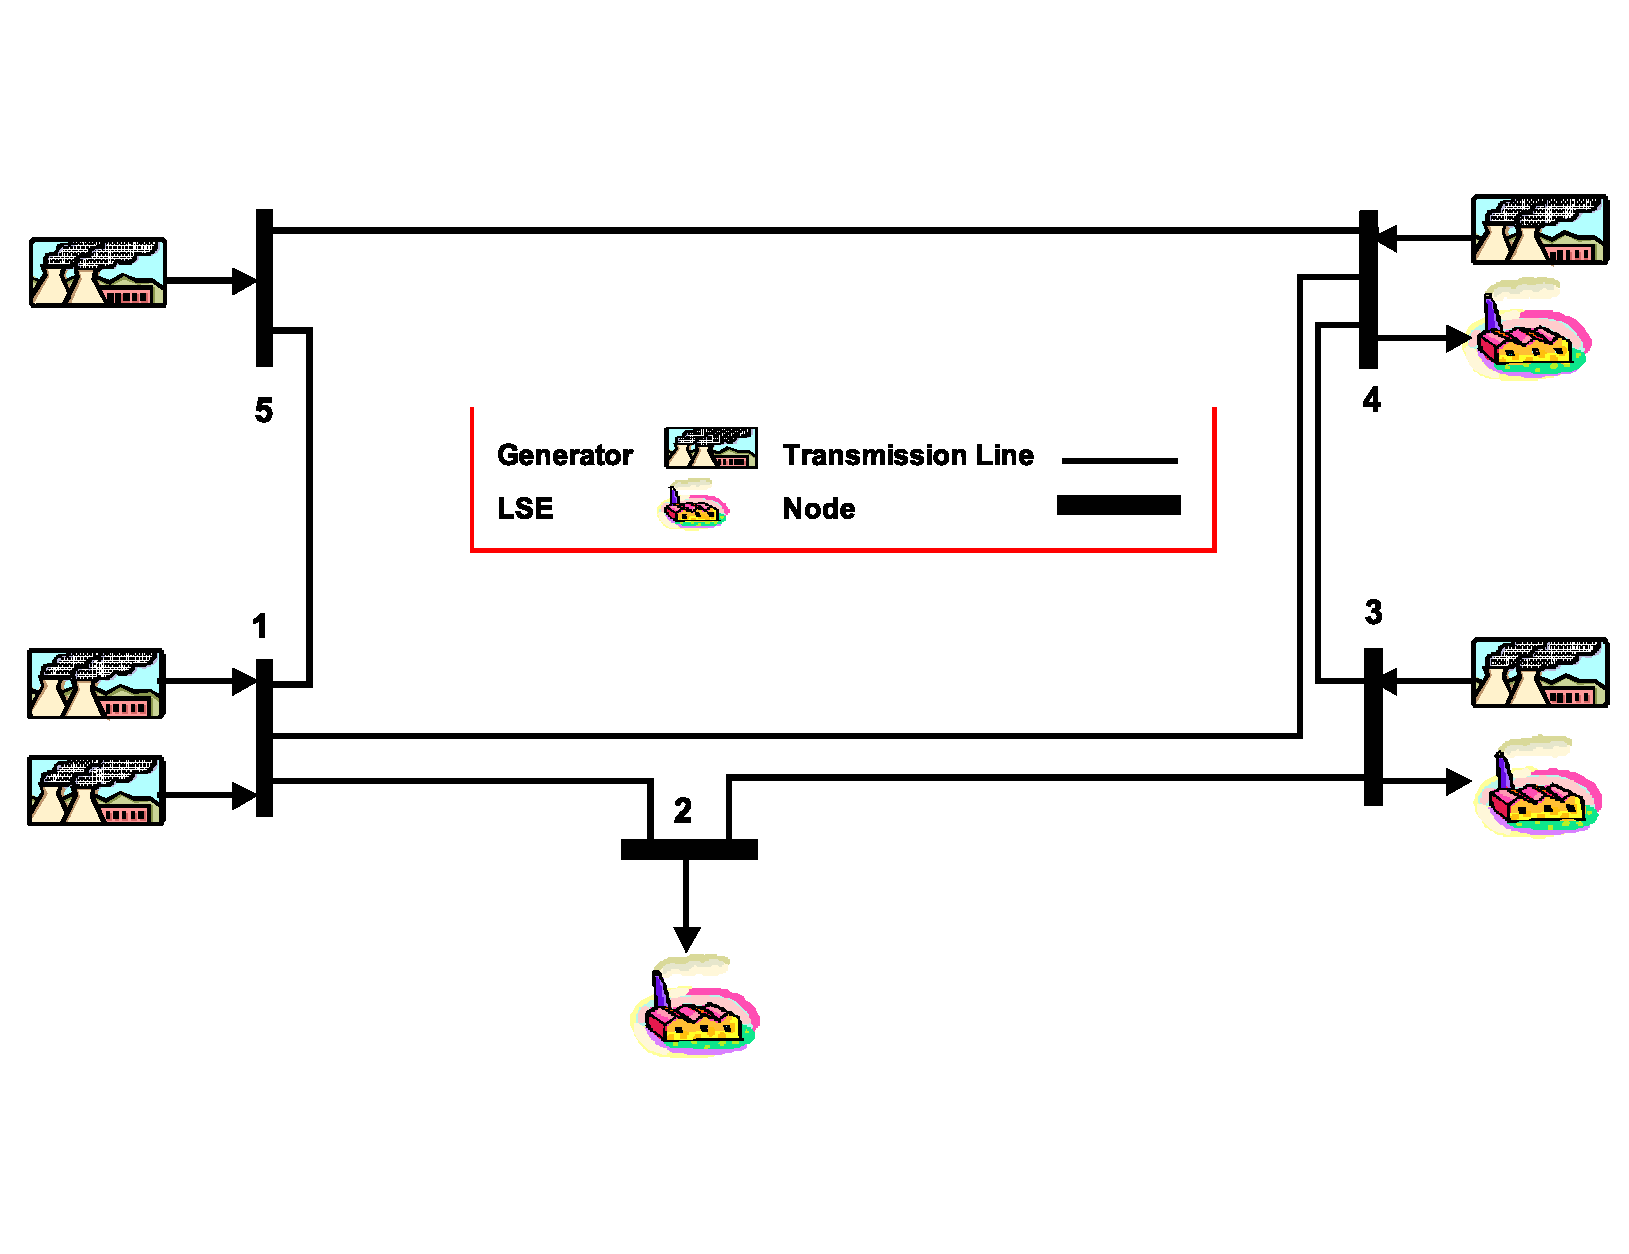
\includegraphics[totalheight = 9cm]{AMES.TransGrid.eps}
	\caption{Illustrative 5-Node Transmission Grid}
	\label{fig:AMES.TransGrid}
\end{figure}  


\begin{figure}
	\centering
		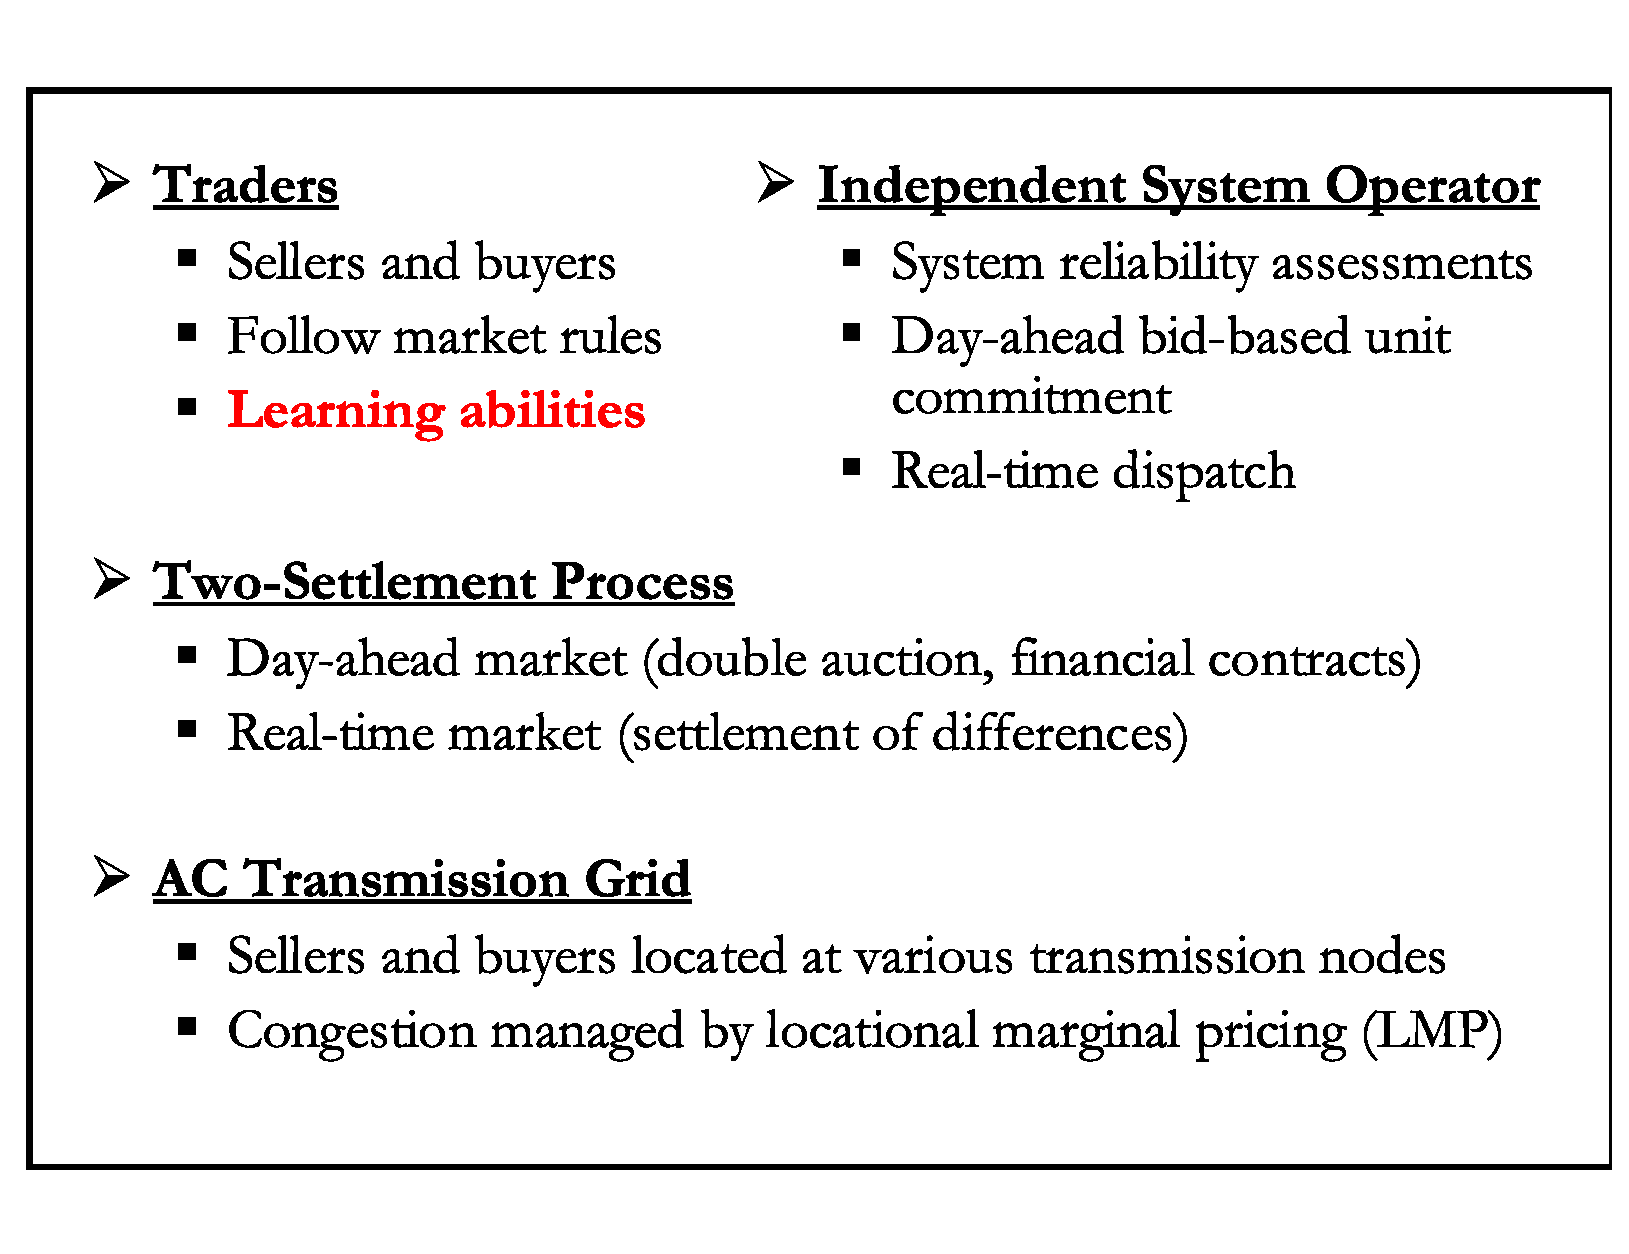
\includegraphics[totalheight = 9cm]{AMES.core.eps}
	\caption{AMES Core Features}
	\label{fig:AMES.core}
\end{figure}  

\begin{figure}
	\centering
		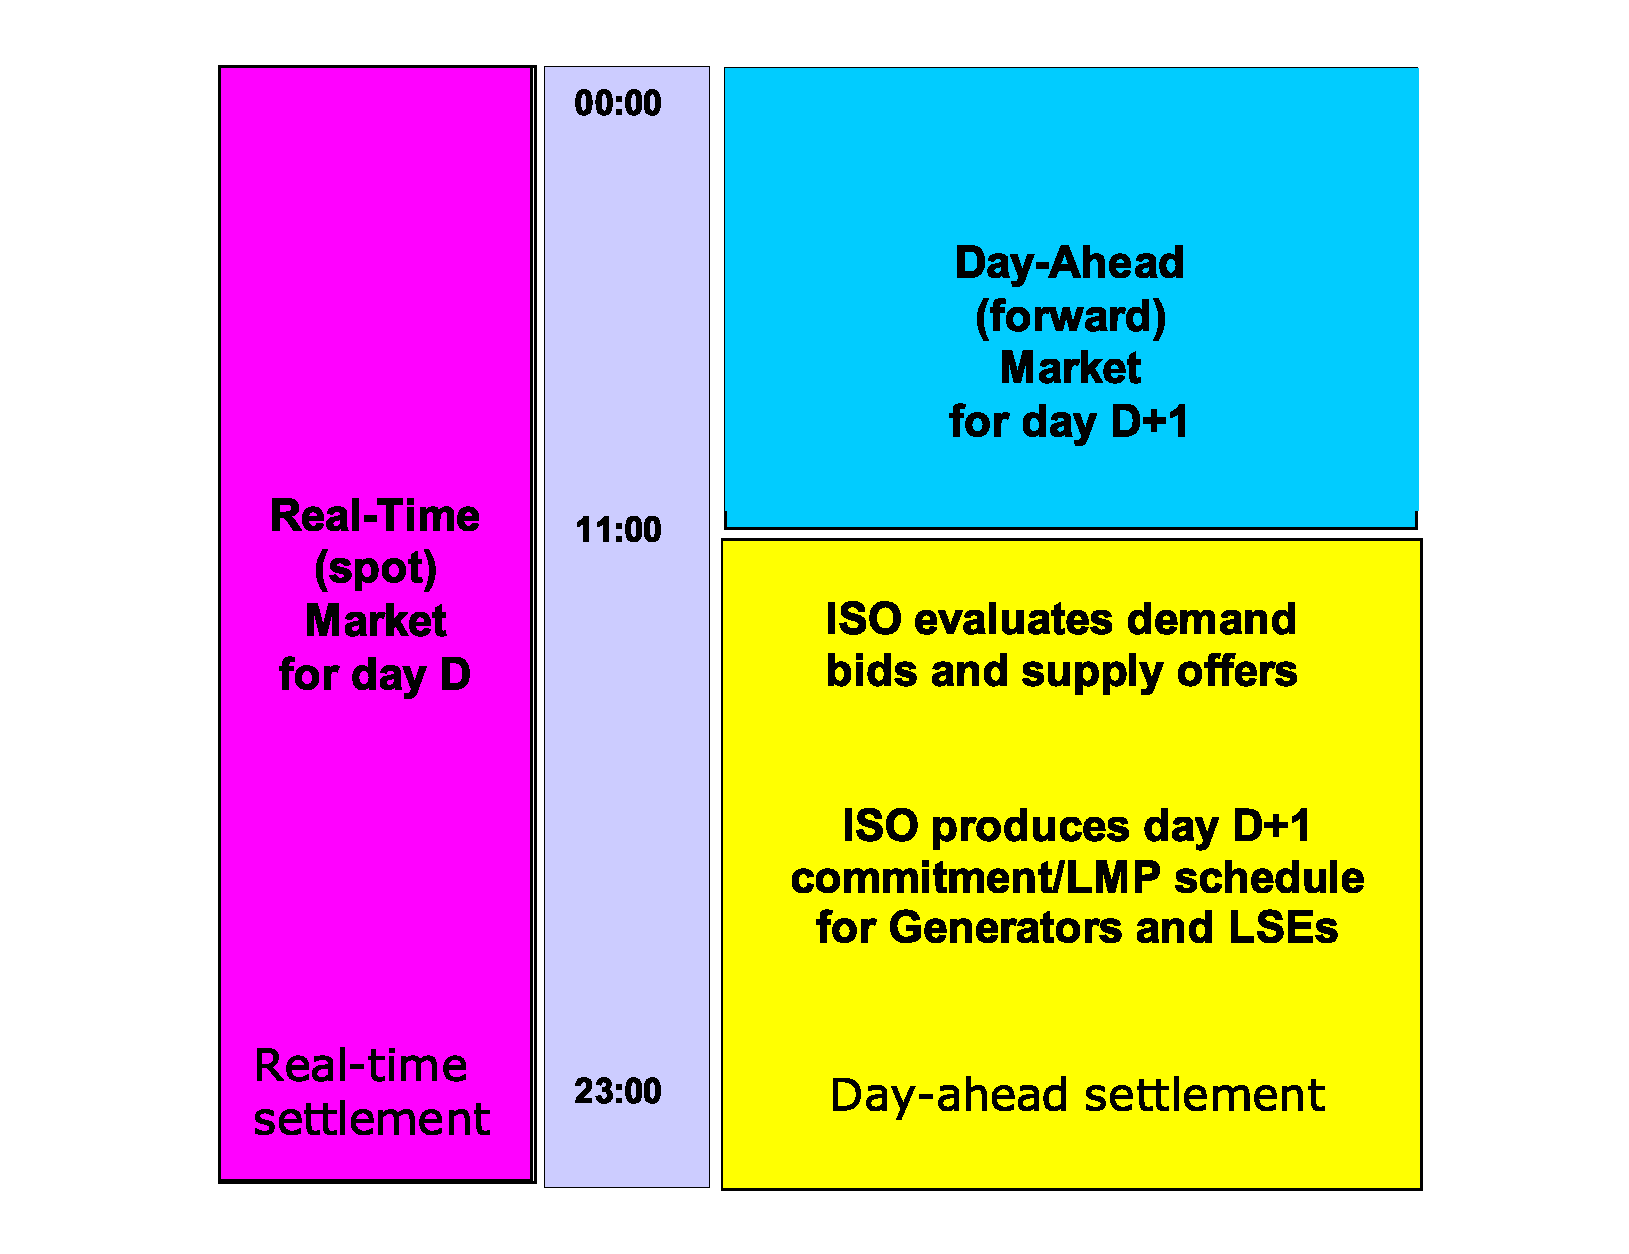
\includegraphics[totalheight = 9cm]{AMES.ISOEvent.eps}
	\caption{Activities of the AMES ISO During a Typical Day D}
	\label{fig:AMES.ISOEvent}
\end{figure}  


Five additional elements that will subsequently be incorporated into AMES to reflect more
fully the dynamic operational capabilities of the WPMP market design are: (a) \textit{market power mitigation 
measures\/}; (b) \textit{bilateral trading\/}, which permits longer-term contracting; (c) a market for
\textit{financial transmission rights\/}%
     \footnote{A \textit{financial transmission right (FTR)} purchased on a transmission line \textit{from\/} 
      node A \textit{to\/} node B entitles the holder to a compensation if the LMP at node B exceeds the LMP 
      at node A, and obligates the holder to make a payment 
      if the LMP at node A exceeds the LMP at node B. See Sun (2006).}
to permit AMES traders to hedge against transmission congestion costs arising in the Day-Ahead 
Market; (d) \textit{security constraints\/} incorporated into the DC OPF problems solved by the AMES ISO for 
the Real-Time Market and Day-Ahead Market as a hedge against system disturbances; and (e) a \textit{(Resource Offer) Re-Bid Period\/}%
     \footnote{Here we follow the MISO market architecture and terminology.  The ISO-NE implements a similar
         design feature during each day D called the ``(Real-Time Energy Market) Supply Re-Offer Period."} 
during each day D as part of a resource adequacy assessment undertaken by the AMES ISO 
to help ensure that forecasted loads and reserve requirements are always met.        
  Figures~\ref{fig:AMES.architecture} and \ref{fig:AMES.SimpleView} schematically depict the architecture and dynamic flow of this extended AMES framework.
 
%%%%%%%%%%%%%%%%%%%%%%%%%%%%%%%%%%%%%%%%%%%%%%%%%%%%%%%%%%
\begin{figure}
	\centering
		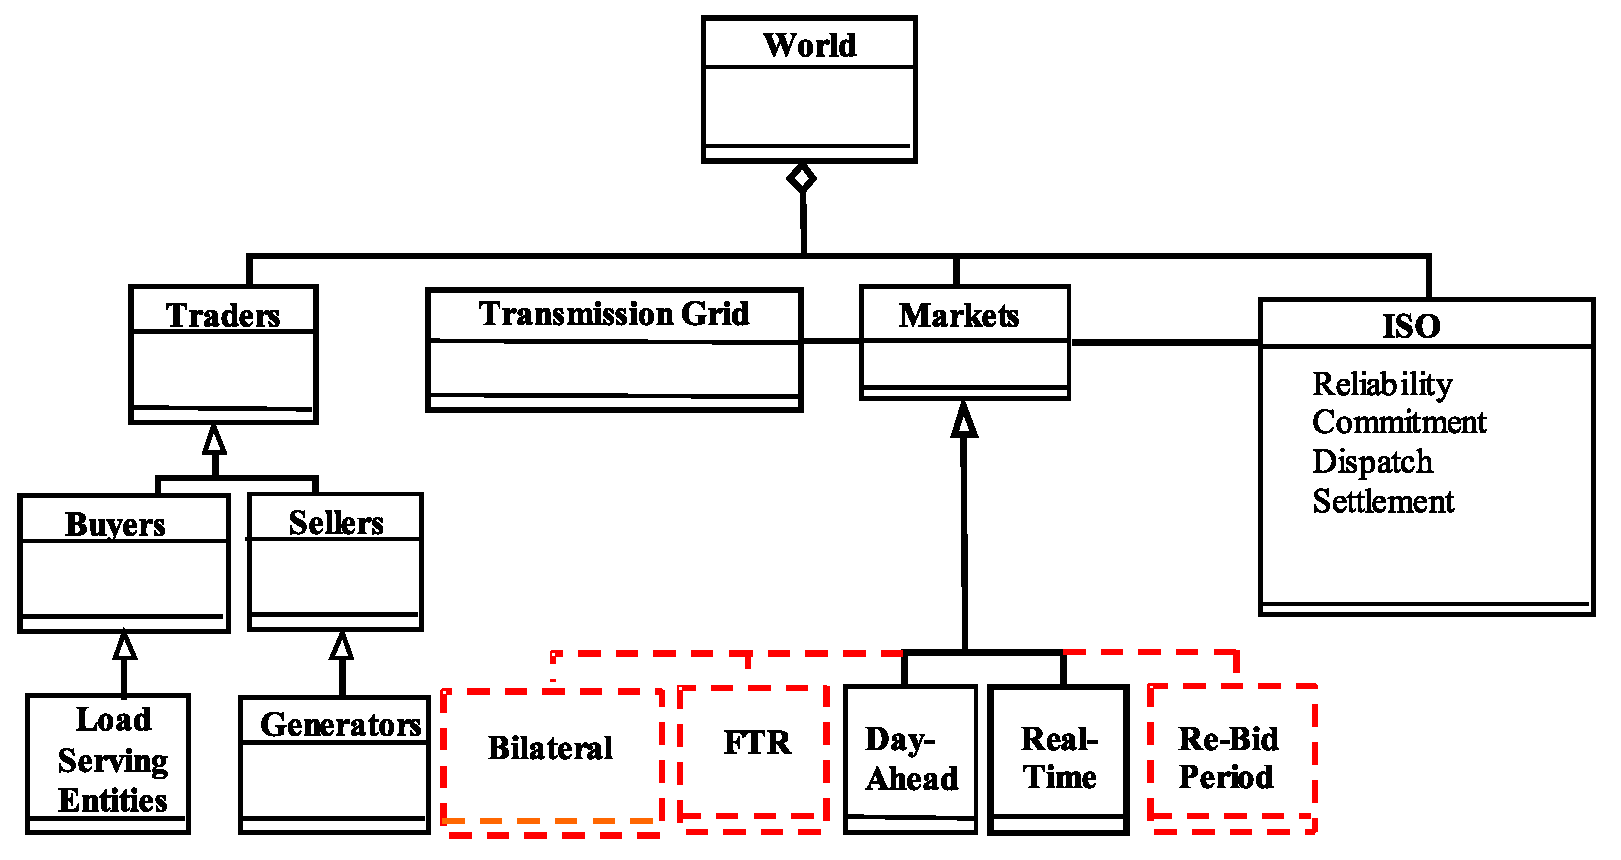
\includegraphics[totalheight = 9cm]{AMES.architecture.eps}
	\caption{AMES Architecture (Agent Hierarchy)}
	\label{fig:AMES.architecture}
\end{figure}  

\begin{figure}
	\centering
		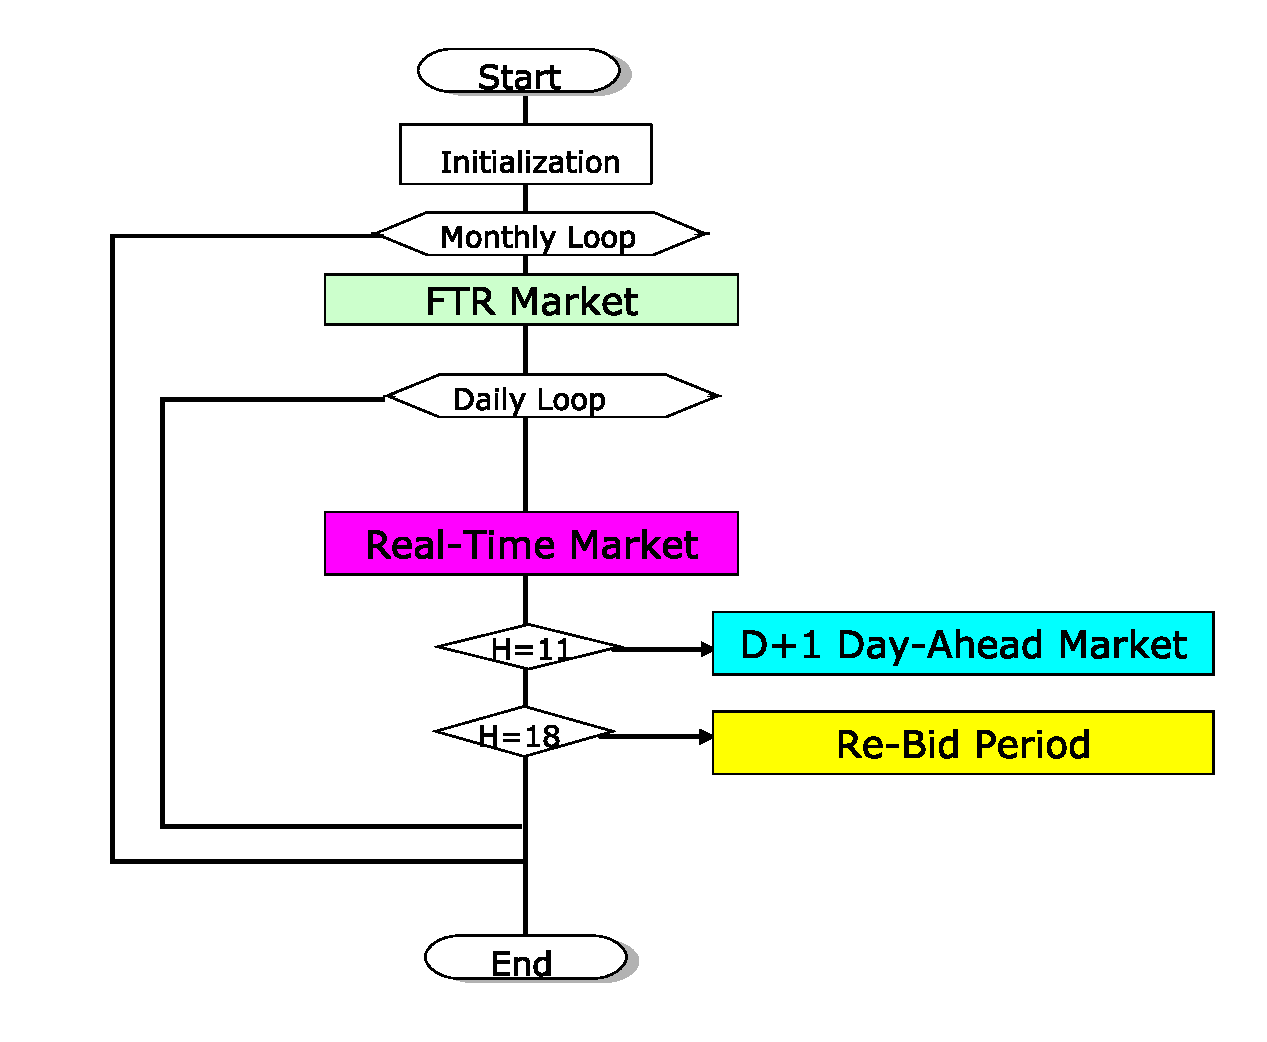
\includegraphics[totalheight = 9cm]{AMES.SimpleView.eps}
	\caption{AMES Dynamic Market Activities: Global View}
	\label{fig:AMES.SimpleView}
\end{figure}      
%%%%%%%%%%%%%%%%%%%%%%%%%%%%%%%%%%%%%%%%%%%%%%%%%%%%%%%%%

As explained more carefully in Section~\ref{ISOConfig} below, the AMES ISO determines hourly power commitments/dispatch levels and LMPs for the Day-Ahead Market and Real-Time Market by solving \textit{DC Optimal Power Flow (OPF)\/} problems that approximate underlying AC OPF problems. To handle these aspects, we have developed an accurate and efficient strictly convex quadratic programming (SCQP) solver module, \textit{QuadProgJ\/}, wrapped in an outer DC OPF data conversion shell, \textit{DCOPFJ} (Sun and Tesfatsion, 2007a,b).  The AMES ISO solves its DC OPF problems by invoking QuadProgJ through DCOPFJ. 

As detailed in Section~\ref{TraderLearning} below, trader learning is implemented in the AMES framework by a reinforcement learning module, \textit{JReLM\/}, developed by Gieseler (2005).  JReLM can implement a variety of different reinforcement learning methods, permitting flexible representation of trader learning within this family of methods.  In later extensions of AMES, other possible trader learning methods (e.g. social mimicry and belief learning) will also be considered.

The QuadProgJ/DCOPFJ and JReLM modules for ISO grid operation and trader learning constitute the core components supporting the implementation of the AMES wholesale power market framework.  This implementation is schematically depicted in Figure \ref{fig:AMES.MainComponents}.

%%%%%%%%%%%%%%%%%%%%%%%%%%%%%%%%%%%%%%%%
\begin{figure}
	\centering
		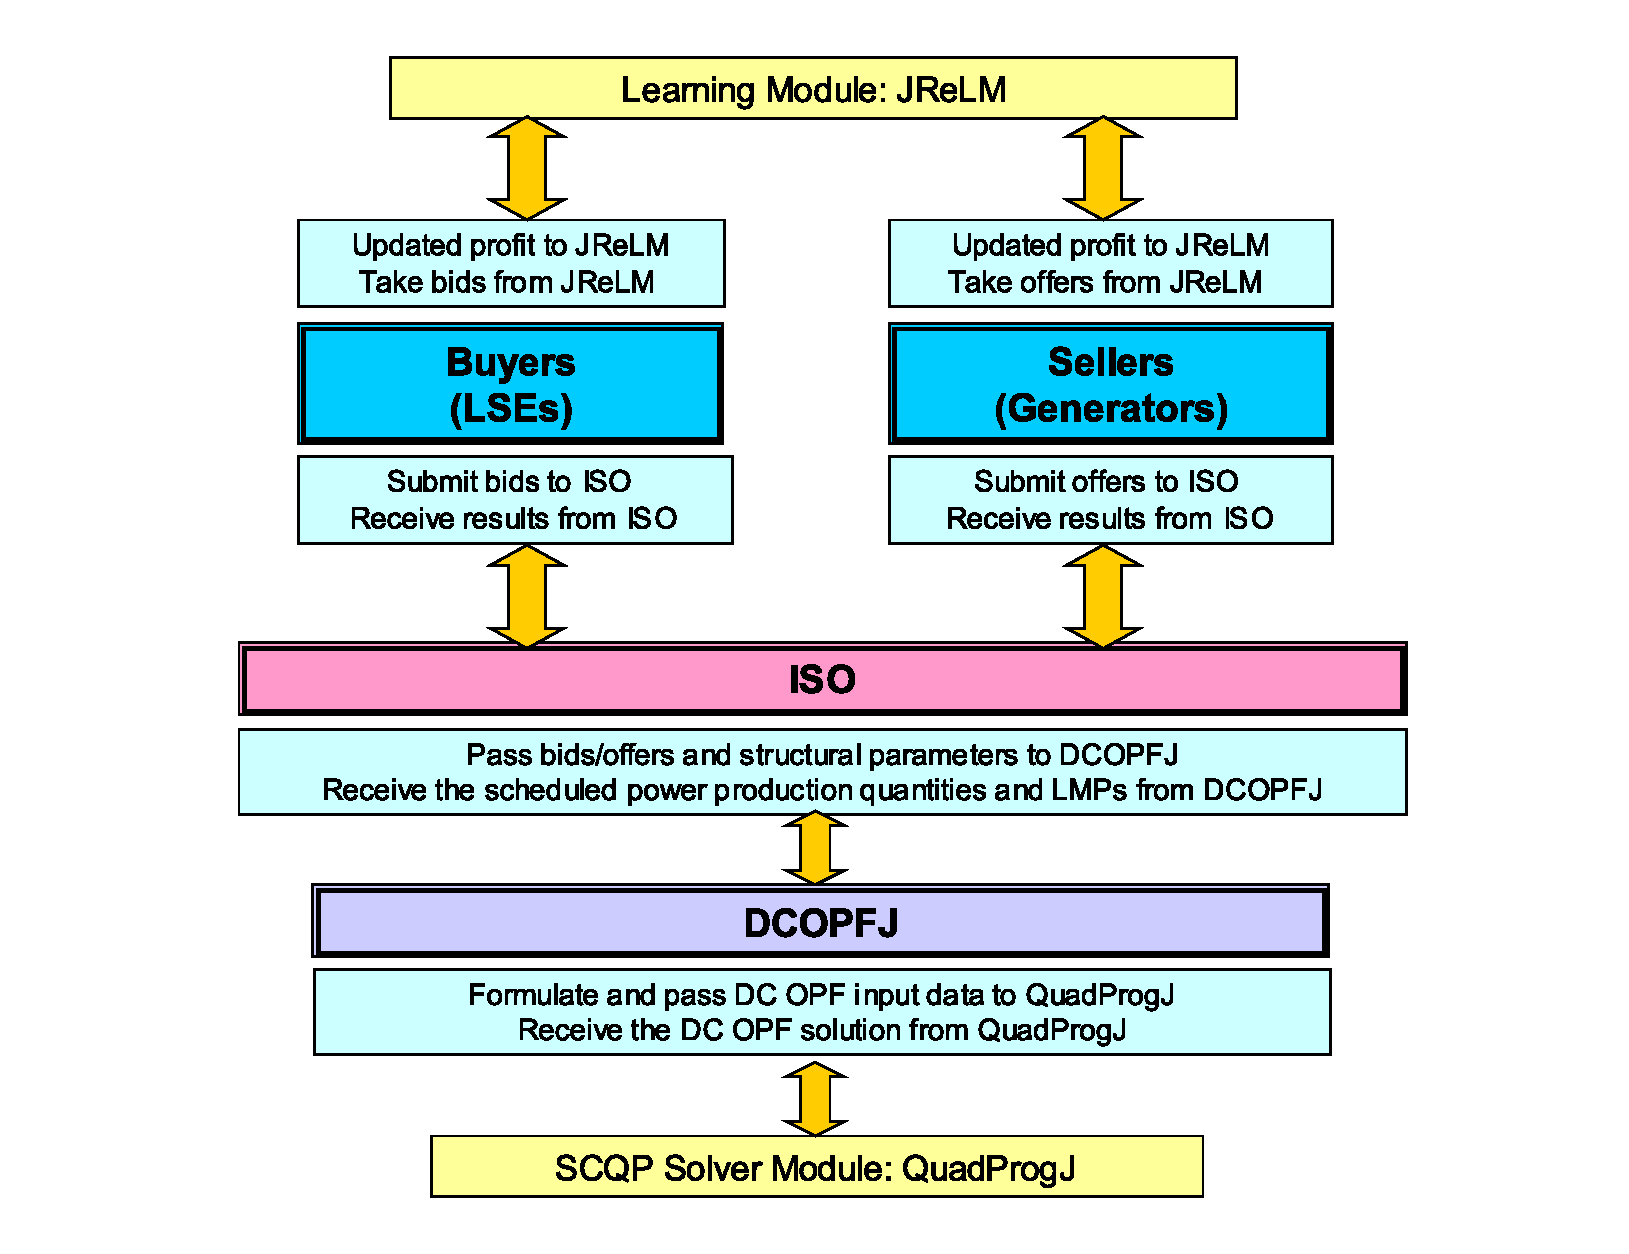
\includegraphics[totalheight = 9cm]{AMES.MainComponents.eps}
	\caption{Core Module Components of the AMES Framework}
	\label{fig:AMES.MainComponents}
\end{figure} 
%%%%%%%%%%%%%%%%%%%%%%%%%%%%%%%%%%%%%%%%



%%%%%%%%%%%%%%%%%%%%%%%%%%%%%%%%%%%%%%%%%%%%%%%%%%%%%%%%%%
%%%%%%%  SECTION  %%%%%%%%%%%%%%%%%%%%%%%%%%%%%%%%%%%%%%%%
%%%%%%%%%%%%%%%%%%%%%%%%%%%%%%%%%%%%%%%%%%%%%%%%%%%%%%%%%%

\section{Configuration of the AMES Framework \label{AMESConfig} }


\subsection{Overview \label{classification} }

This section provides detailed configuration information for the AMES wholesale power market framework as currently implemented.  All subsequently reported experiments make use of these configurations.

For later ease of reference, the admissible exogenous variables for the AMES framework are depicted and defined in 
Table~\ref{tab:ExogVarAdmissibility} and the endogenous variables are depicted and defined in 
Table~\ref{tab:EndogVariables}.%
    \footnote{Only persistent variables appear in these tables.  Locally scoped variables temporarily introduced to carry out method implementations are not included.}
    These variable depictions and definitions will be used throughout the remainder of this study.

\subsection{Structural Configuration of the AMES Transmission Grid \label{InitGrid} }

\noindent
The structural specification of transmission grids is complicated due to the underlying physical relations governing power flows.  Below we briefly summarize the AMES grid specification to indicate the care that has been taken to properly account for these underlying relations.  The interested reader is referred to Sun and Tesfatsion (2007a) and references therein for a more complete and rigorous discussion of this specification.

The AMES transmission grid is an alternating current (AC) grid modeled as a
balanced three-phase network with $N\ge 1$ branches and $K \ge 2$ nodes. 
The reactance on each branch is assumed to be a total branch reactance (rather than a per mile 
reactance), meaning that the branch length is already taken into account. All transformer 
phase angle shifts are assumed to be zero, all transformer tap ratios are assumed 
to be 1, all line-charging capacitances are assumed to be 0, and the temperature is 
assumed to remain constant over time.

    The AMES transmission grid is assumed to be
\textit{connected\/} in the sense that it has no isolated components; each
pair of nodes $k$ and $m$ is connected by a linked branch path consisting of one or 
more branches.  If two nodes are in direct connection
with each other, it is assumed to be through at most one branch, i.e., branch groups 
are not explicitly considered.
     However, complete connectivity is \textit{not\/} assumed. 
That is, node pairs are \textit{not\/} necessarily in \textit{direct\/} connection with each other 
through a single branch.  

For per unit normalization in DC OPF implementations, it is conventional to specify base value 
settings for apparent power (in megavoltamperes MVA) and voltage (in kilovolts kV).
For the AMES transmission grid, the base apparent power, denoted by $S_o$, is assumed to be 
measured in three-phase MVAs, and the base voltage, denoted by $V_o$, is assumed to be measured in line-to-line kVs.   

It is also assumed that {\it Kirchoff's Current Law (KCL)\/} governing current flows in electrical networks
holds for the AMES transmission grid for each hour of operation.  As detailed
in Kirschen and Strbac (2004, Sec.~6.2.2.1), KCL implies that real and
reactive power must each be in balance at each node.  Thus, real power must
also be in balance across the entire grid, in the sense that aggregate real
power withdrawal plus aggregate transmission losses must equal aggregate real
power injection.  

In wholesale power markets restructured in accordance with the WPMP market design, 
the transmission grid is overlaid with a commercial 
network consisting of
``pricing locations'' for the purchase and sale of electric power.  A {\it pricing 
location\/} 
is a location at which market transactions are 
settled using publicly available LMPs. 
For simplicity, it is assumed that the set of pricing locations for AMES coincides with the set of 
transmission grid nodes.

\subsection{Structural Configuration of the AMES LSEs \label{LSEConfig} }

\noindent
The AMES LSEs purchase bulk power in the AMES wholesale power market each day in order 
to service customer demand (load) in a downstream retail market.
The user specifies the number $J$ of LSEs as well as the location of these
LSEs at various nodes of the transmission grid.  LSEs do not engage in
production or sale activities in the wholesale power market.  
Hence, LSEs purchase power only from Generators, not from each other.

For initial simplicity, the current study makes the usual empirically-based assumption that the downstream 
retail demands serviced by the AMES LSEs exhibit negligible price sensitivity and hence reduce to daily load profiles. 
In addition, the LSEs are modeled as
passive entities who submit these  
daily load profiles into the Day-Ahead Market as their demand bids without strategic consideration.
Specifically, at the beginning of each day D each LSE $j$ submits a daily load profile 
into the day-ahead market for day D+1 .  This daily load profile 
indicates the real power demand $p_{Lj}(\mbox{H})$ (in MWs) that must be serviced by LSE $j$ in its downstream 
retail market for each of 24 successive hours H.  


\subsection{Structural Configuration of the AMES Generators \label{GenConfig} }

\medskip
\noindent
The AMES Generators are electric power generating units. 
The user specifies the number $I$ of
Generators as well as the location of these Generators at various nodes of
the transmission grid.  Generators sell power only to LSEs, not to each
other.  Each AMES Generator $i$ is user-configured with a 
production technology, learning capabilities, and an initial 
level $\mbox{Money}^o_{i}$ of money holdings.  Here we elaborate on Generator 
production technologies; learning capabilities are separately taken up in 
Subsection~\ref{TraderLearning} below.

With regard to production technology, it is assumed 
that each Generator has variable 
and fixed costs of production.  However, Generators do not incur no-load, startup, or shutdown costs, and 
they do not face ramping constraints.%
         \footnote{As is standard in economics, {\it variable costs\/} are
costs that vary with the level of production, and {\it fixed costs\/} are
costs such as debt and equity obligations associated with plant investments
that are not dependent on the level of production and that are incurred 
even if production ceases.  As detailed by Kirschen and Strbac (2004, Sec.~4.3), 
the concept of {\it no-load costs\/} 
in power engineering refers to \textit{quasi-fixed\/} costs that would be incurred by Generators 
if they could be kept running at zero output but that would vanish once
shut-down occurs.  {\it Startup costs\/} are costs specifically incurred 
when a Generator starts up, and \textit{shutdown costs\/} are costs specifically incurred when 
a Generator shuts down.  Finally, \textit{ramping constraints\/} refer to physical
restrictions on the rates at which Generators can increase or decrease their
outputs.}

   More precisely, the technology attributes assumed for each Generator $i$ take the following form.
Generator $i$ has lower and upper production limits (in MWs), denoted by $\mbox{Cap}^L_{i}$ 
and $\mbox{Cap}^U_{i}$,
that define the \textit{feasible production interval\/} 
for its hourly real-power production level
$p_{Gi}$ (in MWs).%
    \footnote{In the current AMES modeling, the lower production limit $\mbox{Cap}^L_{i}$ 
for each Generator $i$ is a firm ``must run" minimum real-power production level.  
That is, if $\mbox{Cap}^L_{i}$ is positive, then shutting down Generator $i$ is not an option 
for the AMES ISO.  Consequently, for most applications of AMES, these lower production limits 
should be set to zero.\label{FirmLowerProdLimits} }                         
     That is, for each $i$,
              \begin{equation}  \label{TruePI}
     \mbox{Cap}^L_{i} ~~ \le ~~ p_{Gi} ~~ \le ~~ \mbox{Cap}^U_{i}
                \end{equation}
In addition, Generator $i$ has a {\it total cost function\/} giving its
total costs of production per hour for each $p_{Gi}$.  This total 
cost function takes the form

                 \begin{equation} \label{TotalCost}
     \mbox{TC}_i(p_{Gi}) ~ = ~ a_i\cdot p_{Gi}
                             ~+~ b_i\cdot p_{Gi}^2 ~+~ \mbox{FCost}_i
                    \end{equation}                  
where $a_i$ ($\$$/MWh), $b_i$ ($\$$/MW$^2$h), and
$\mbox{FCost}_i$ ($\$$/h) are exogenously given constants. 
Note that $\mbox{TC}_i(p_{Gi})$ is measured in dollars per hour ($\$/h$).
Generator $i$'s \textit{total variable cost function\/} and \textit{(hourly prorated) fixed
costs} for any $p_{Gi}$ are then given by%
		\footnote{Quadratic functions as in (\ref{TotalVariableCost}) are commonly used to represent generator total variable costs (i.e. costs of operation) in power systems research; for example, see Shahidehpour et al.~(2002).  Variable costs in actual wholesale power markets primarily reflect fuel and labor costs, and additional study is needed to gauge the extent to which quadratic functions can adequately represent these costs.}
     \begin{equation} \label{TotalVariableCost}
          \mbox{TVC}_i(p_{Gi}) ~ = ~ \mbox{TC}_i(p_{Gi}) - \mbox{TC}_i(0) ~=~ ~ a_i\cdot p_{Gi}
                             ~+~ b_i\cdot p^2_{Gi} 
      \end{equation}
and 
             \begin{equation}
       \mbox{FCost}_i ~ = ~ \mbox{TC}_i(0)
              \end{equation}
respectively.  Finally, the \textit{marginal cost function\/} for Generator $i$ takes the form
              \begin{equation} \label{MarginalCost}
     \mbox{MC}_i(p_{Gi}) ~ = ~ a_i  ~+~ 2\cdot b_i\cdot p_{Gi}
                    \end{equation}

At the beginning of each day D, each Generator $i$ reports a \textit{supply offer\/} $s^R_i(\mbox{D})$ to the AMES ISO for use in each hour H of the Day-Ahead Market for day D+1 .  This supply offer consists of a \textit{reported marginal cost function\/} (i.e.\ \textit{supply schedule\/})
                 \begin{equation} \label{ReportedMC}
     \mbox{MC}^R_i(p_{Gi}) ~ = ~ a^R_i  ~+~ 2\cdot b^R_i\cdot p_{Gi}
                      \end{equation}
defined over a \textit{reported feasible production interval\/}%
          \footnote{As emphasized by Cain and Alvarado~(2004), the implications of supply offer formats for the operation of wholesale power markets is an important topic in need of further study.  Here we follow the basic form of the generator supply offers required by the MISO (2007) and ISO-NE (2007): namely, non-decreasing supply schedules accompanied by minimum and maximum real power production capacities.  However, we assume \textit{linear\/} supply schedules to ease the specification of the learning problem for the AMES Generators whereas the MISO and ISO-NE require step-function supply schedules. (Interestingly, in the ISO-NE the generators can check a ``UseOfferSlope" box permitting the ISO to approximate their step-function supply schedules by smoother curves.) In addition, for initial simplicity, we follow the current practice of the ISO-NE in only permitting the AMES Generators to submit \textit{one\/} supply offer to be used for \textit{each\/} hour of the Day-Ahead Market, whereas the MISO permits generators to submit a separate supply offer for each hour of the Day-Ahead Market.}
 
                  \begin{equation} \label{ReportedPI}
     \mbox{Cap}^{RL}_{i} ~~ \le ~~ p_{Gi} ~~ \le ~~ \mbox{Cap}^{RU}_{i}
                  \end{equation}
  This supply offer can be \textit{strategic\/} in the sense that the reported cost coefficients $a^R_i$ and $b^R_i$ in 
(\ref{ReportedMC}) can deviate from Generator $i$'s true cost coefficients $a_i$ and $b_i$ in (\ref{MarginalCost}) and the reported feasible production interval $[\mbox{Cap}^{RL}_i,\mbox{Cap}^{RU}_i]$ in (\ref{ReportedPI}) can deviate from Generator $i$'s true feasible production interval $[\mbox{Cap}^{L}_i,\mbox{Cap}^{U}_i]$ in (\ref{TruePI}).
         
Suppose Generator $i$ is located at node $k$, and suppose Generator $i$ in some day D reports a supply 
offer $s^R_i(\mbox{D})$ to the AMES ISO for the day D+1 Day-Ahead Market (along with all other Generators).  Let $LMP_k$ denote the node-$k$ locational marginal price (LMP) that is then subsequently determined by the AMES ISO in day D for some hour H of day D+1, and let $p^\ast_{Gi}$ denote the real power that Generator $i$ has been 
cleared to inject at node $k$ in hour H of day D+1 .  Then the (possibly negative) profit accruing to Generator $i$ in day D from the day-$D$ settlement of this financially binding contract for hour H of day D+1  is

\begin{equation} \label{Profits}
	\mbox{Profit}^{\mbox{new}}_i(p^\ast_{Gi})~ = ~ \mbox{LMP}_k \cdot p^\ast_{Gi} - \mbox{TC}_i(p^\ast_{Gi})
\end{equation}


\noindent
Moreover, as a result of this settlement, the updated cumulated money holdings for Generator $i$ are given by

\begin{equation} \label{MoneyDynamics}
	\mbox{Money}_i^{\mbox{new}} ~ =  ~ \mbox{Money}_i^{\mbox{prev}}~ + ~~\mbox{Profit}^{\mbox{new}}_i(p^\ast_{Gi})
\end{equation}


\medskip
\noindent
Since Generator $i$'s profits (\ref{Profits}) can be negative, it is clear from (\ref{MoneyDynamics}) that Generator $i$ faces a risk of \textit{insolvency}, i.e., a risk that its money holdings will run out. Any Generator that becomes insolvent must immediately exit the market, which results in the loss of its production capacity to the market. Furthermore, no entry of new generation is permitted in the current implementation of the AMES framework.

%%%%%%%%%%%%%%%%%%%%%%%%%%%%%%%%%%%%%%%%%%%%%%%%%%%%%%%%%%%%%%%%%%


\subsection{Structural Configuration of the ISO \label{ISOConfig} }

As in actual ISO-managed wholesale power markets operating under the WPMP market design, the AMES ISO during each day D is charged with determining a schedule of optimal power commitments and LMPs for each hour of the Day-Ahead Market in day D+1.  This schedule is conditional on LSE-reported demand bids, Generator-reported supply offers, thermal limits on branch flows, and nodal balance constraints ensuring supply equals demand (load) at each transmission grid node.  

As usual, ``optimal" is interpreted to mean that total net surplus is maximized.  The resulting optimization problem is known as a \textit{bid-based AC optimal power flow (OPF)\/} problem.  As typically done in actual markets, the AMES ISO approximates this difficult bid-based AC OPF problem by means of a simpler bid-based DC OPF problem in which real power constraints are linearized and reactive power constraints are ignored. A brief discussion of this bid-based DC-OPF problem will now be given.%
     \footnote{Sun and Tesfatsion~(2007a) motivate in detail the form of the objective function and constraints for this bid-based DC-OPF problem as well as explaining carefully how it is derived from an AC-OPF problem given certain standard simplifying assumptions.}
       
Recall from Section~\ref{LSEConfig} that the AMES LSEs are currently modeled as non-strategic entities servicing price-insensitive loads whose reported demand bids in each day D take the form of their true daily load profiles. In this case the maximization of total net surplus reduces to the minimization of Generator-reported total variable cost.  Using the variable definitions in Tables~\ref{tab:ExogVarAdmissibility} and \ref{tab:EndogVariables}, the bid-based DC OPF problem solved by the AMES ISO in day D for each hour of the Day-Ahead Market in day D+1 is then as follows:

\bigskip
\noindent \textbf{Minimize Generator-reported total variable cost}
\begin{equation} \label{DCOPFObjective}
	\sum_{i=1}^I [a^R_i p_{Gi} + b^R_i p_{Gi}^2 ]
\end{equation}

\noindent \textbf{with respect to real-power production levels and voltage angles}
\[ p_{Gi},~ i=1,...,I;~~~ \delta_k,~ k=1,...,K\] 


\noindent \textbf{subject to:}\\
\newline
\indent\textbf{Real power balance constraint for each node $\mathbf{k=1,...,K}$:}

                   \begin{equation} \label{dcPBalancek}
     0 ~ = ~  \mbox{PLoad}_k  ~ - ~
                 \mbox{PGen}_k ~ + ~ \mbox{PNetInject}_k 
                      \end{equation}
 \indent   where

                       \begin{equation}
             \mbox{PLoad}_k ~ = ~ \sum_{j \in J_k} \, p_{Lj} 
                       \end{equation}

                              \begin{equation}
             \mbox{PGen}_k ~ = ~ \sum_{i \in I_k} \, p_{Gi} 
                      \end{equation}

           \begin{equation}  \label{dcNetInject2}
    \mbox{PNetInject}_k ~~ = ~~ \sum_{km\,\mbox{\footnotesize or}\,mk\in BR} P_{km} 
    \end{equation}

\begin{equation}  \label{dcPowerFlow}
       P_{km} ~~ = ~~ B_{km}[V_o]^2~[ \delta_{k} - \delta_{m}]
\end{equation}

\vspace{10pt}
\textbf{Real power thermal constraints for each branch $\mathbf{km \in BR}$:}

\begin{equation}  \label{dcSkmLimit}
|P_{km}|  ~~  \le  ~~ P^U_{km}
\end{equation}

\vspace{10pt}
\textbf{Reported real-power production constraints for each Generator $\mathbf{i=1,..,I}$:}

               \begin{equation}  \label{dcPCapLimits}
         \mbox{Cap}^{RL}_i ~~ \le ~~  p_{Gi} ~~ \le  ~~ \mbox{Cap}^{RU}_i 
                \end{equation}

\vspace{10pt}
\textbf{Voltage angle setting at reference node 1:}

                \begin{equation}  \label{dcDeltaRefBus}
             \delta_{1} ~~ = ~~ 0
                       \end{equation}

\medskip
As shown in Sun and Tesfatsion (2007a), this DC OPF problem can equivalently be represented in the numerically desirable form of a strictly convex quadratic programming (SCQP) problem if the balance constraints (\ref{dcPBalancek}) are used to eliminate the voltage angles $\delta_k$ by substitution.  However, this elimination prevents direct generation of solution values for LMPs since, by definition, the LMP for node $k$ is the solution value for the multiplier (shadow price) for the $k$th nodal balance constraint.  

For this reason, we replace the standard DC OPF objective function (\ref{DCOPFObjective}) with the following augmented 
form:
\begin{equation} \label{DCOPFObjAug}
	\sum_{i=1}^I [a^R_i p_{Gi} + b^R_i p_{Gi}^2 ]~ + ~ \pi \left[ \sum_{km \in BR}  [\delta_k - \delta_m]^2 \right]~,
\end{equation}
  
\smallskip
\noindent
where $\pi$ is a positive soft penalty weight on the sum of squared voltage angle differences.  As carefully demonstrated in Sun and Tesfatsion (2007a), the augmentated DC OPF objective function (\ref{DCOPFObjAug}) provides a number of benefits based on both physical and mathematical considerations.  

First, the resulting augmented DC OPF problem now has a numerically desirable SCQP form permitting the direct generation of solution values for LMPs as well as for real power production levels, branch flows, and voltage angles. Second, the validity of the DC OPF as an approximation for the underlying AC OPF relies on an assumption of small voltage angle differences, and the augmented DC OPF problem permits this assumption to be subjected to systematic sensitivity tests through variations in the penalty weight $\pi$.  Third, solution differences between the non-augmented and augmented forms of the DC OPF problem can be reduced to arbitrarily small levels by selecting an appropriately small value for $\pi$. 

To solve this augmented DC OPF problem, the AMES ISO invokes the SCQP solver QuadProgJ through an outer shell DCOPFJ.  More precisely, as illustrated below in Section~\ref{5NodeTestCase}, the AMES ISO passes to DCOPFJ current DC OPF input data in standard (SI) units together with base apparent power and voltage values $S_o$ and $V_o$.  DCOPFJ converts this SI input data into per unit (pu) form and performs all needed matrix and vector representations.  DCOPFJ then invokes QuadProgJ to solve for LMPs, voltage angles, real power production levels, real power branch flows, and various other useful quantities  with all internal calculation carried out in pu terms.  QuadProgJ then passes these pu solution values back to DCOPFJ, which outputs them in SI units.  

In future studies, the AMES ISO will also have to solve DC OPF problems for the Real-Time Market to settle any differences that arise between day-ahead commitments and real-time conditions due to system disturbances (e.g. sudden line outages or changes in demand).  However, in our initial experiments with the AMES framework we are not considering system disturbances that would cause such differences to arise.  Consequently, all load obligations are fully met through Day-Ahead Market transactions and the Real-Time Market is inactive. 

%%%%%%%%%%%%%%%%%%%%%%%%%%%%%%%%%%%%%%%%%%%%%%%%%%%%%%%%%%
%%%%%%%%%%%%%%%%%%%%%%%%%%%%%%%%%%%%%%%%%%%%%%%%%%%%%%%%%%


\subsection{Learning Configuration for the AMES Generators \label{TraderLearning} }    

In general, multiple Generators at multiple nodes could be under the control of a single 
generation company (``GenCo").  This control aspect is critically important to recognize for 
the study of real-world strategic trading.  This situation can be handled in the AMES framework 
by permitting coordinated learning across Generators controlled by a single GenCo.  

For initial simplicity, however, the AMES Generators are currently modeled as autonomous energy traders 
with strategic learning capabilities; see Figure \ref{fig:AMES.Gen}. Each AMES Generator adaptively selects its supply offers on the basis of its own past profit outcomes using a version of a stochastic reinforcement learning algorithm developed by Roth-Erev (1995) based on human-subject experiments, hereafter referred to as the \textit{VRE learning algorithm\/}.  This section briefly outlines the implementation of the VRE learning algorithm for an arbitrary 
Generator $i$.  

%%%%%%%%%%%%%%%%%%%%%%%%%%5
\begin{figure}
	\centering
		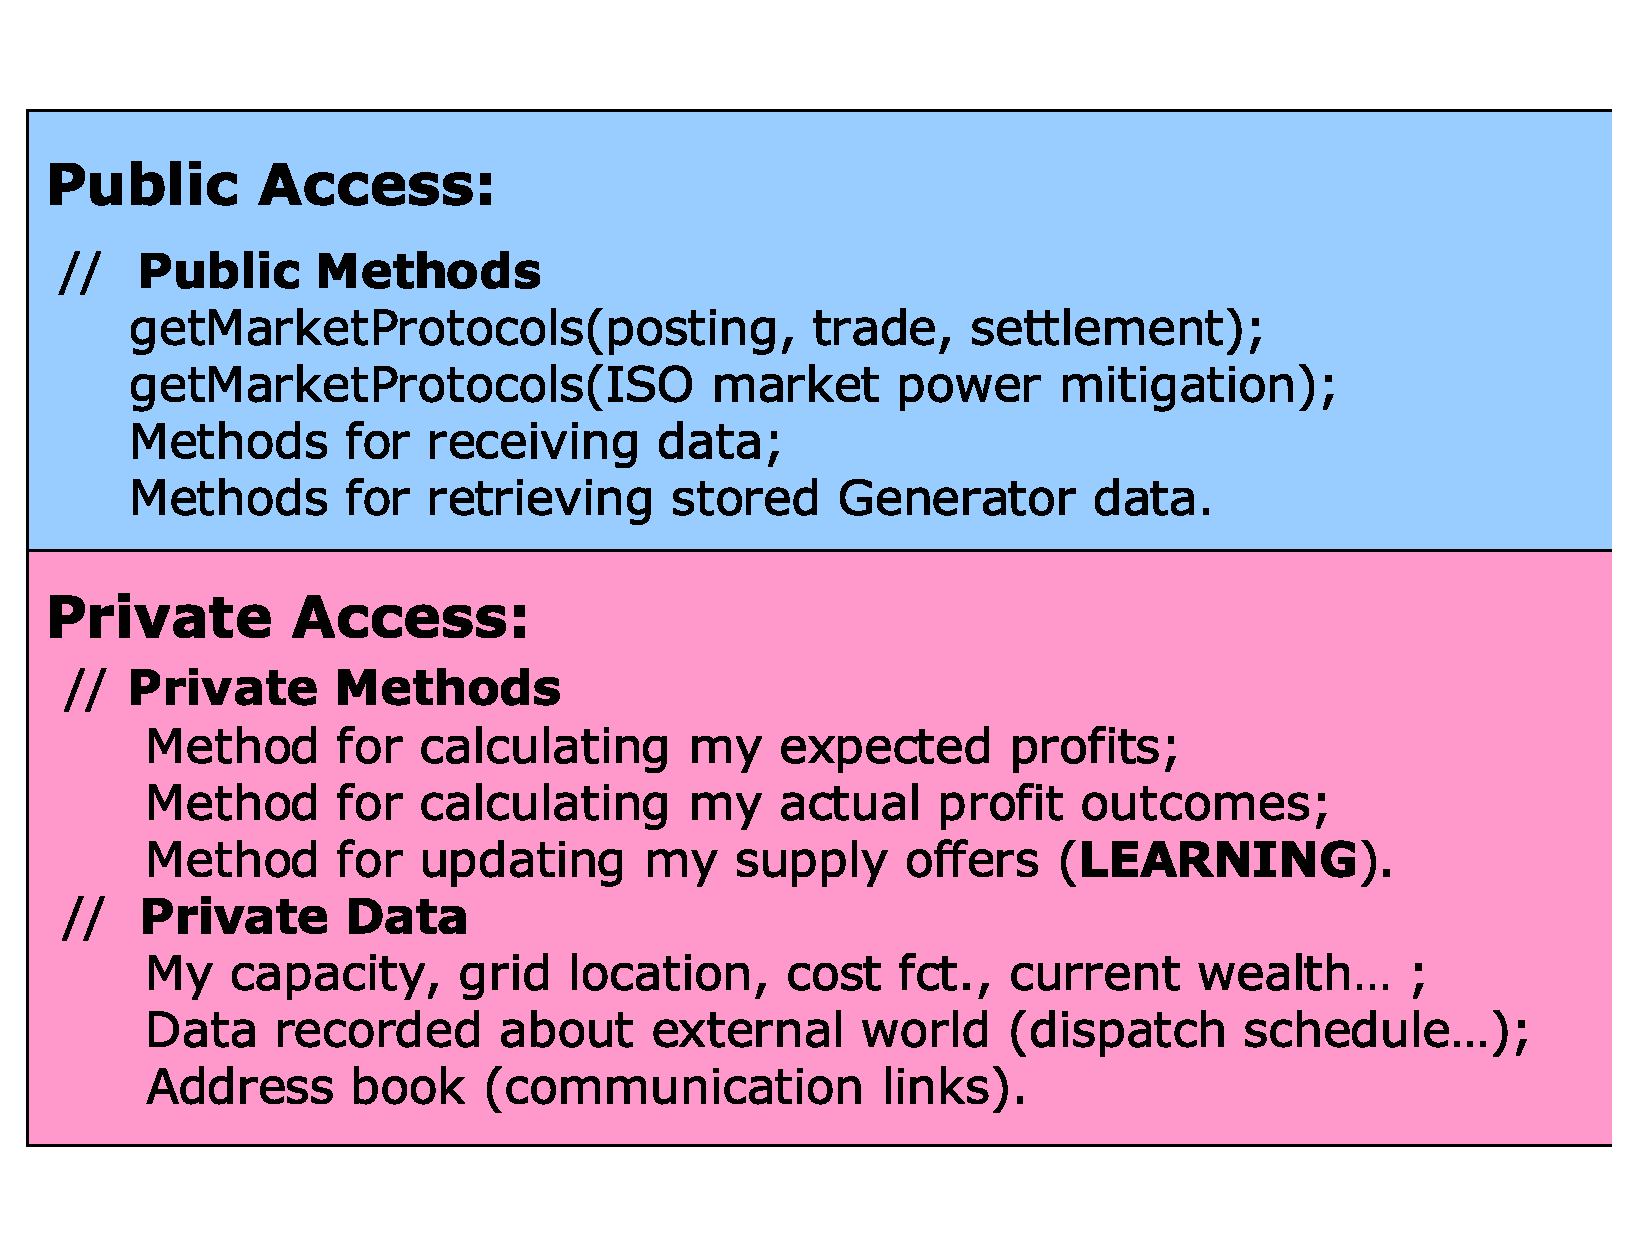
\includegraphics[totalheight = 9cm]{AMES.Gen.eps}
	\caption{A Computational Generator (Seller)}
	\label{fig:AMES.Gen}
\end{figure}  
%%%%%%%%%%%%%%%%%%%%%%%%%%

    Suppose it is the beginning of the initial day D=$1$, and Generator $i$ must choose a supply offer from its 
\textit{action domain $AD_i$\/} to report to the AMES ISO for the Day-Ahead Market in day D+1 .  As will be seen below, for learning purposes the only relevant attribute of $AD_i$ is that it has finite cardinality $M_i \ge 1$.%
        \footnote{Technical details concerning the construction of each Generator $i$'s action domain $AD_i$ are taken up in the appendix. The key issue is how to construct the sets $AD_i$ to give each Generator an economically meaningful and realistically flexible selection of supply offers without introducing hidden structural biases favoring some Generators over others.}
      

    The \textit{initial propensity\/} of Generator $i$ to choose supply offer $m \in AD_i$ is
given by $q_{im}(0)$.  In general, these initial propensities can be 
any real numbers as specified by the AMES user.  However, the default setting used in this study is that these 
initial propensities are equal.  That is, we specify a fixed value $q_{i}(0)$ such that
                    \begin{equation}
     q_{im}(0) ~~ =  ~~q_{i}(0) ~~ \mbox{for all supply offers}~m \in AD_i
                  \label{initprop}
            \end{equation}

     Now consider the beginning of any day D $\ge 1$, and suppose the 
current propensity of Generator $i$ to choose supply offer $m \in AD_i$ is given by
$q_{im}(\mbox{D})$.  The {\it choice probabilities\/} that Generator $i$ uses to
select a supply offer for day D are then constructed from these propensities as follows:%
        \footnote{In the original algorithm developed by Erev and
Roth~(1998) and Roth and Erev~(1995), the choice probabilities
are defined in terms of relative propensity levels.  Here, instead, use is
made of a ``simulated annealing'' formulation in terms of exponentials.  As
will be seen below in (\ref{update}), in the current context the propensity
values can take on negative values if sufficiently large negative profit
outcomes are experienced, and the use of exponentials ensures that the choice
probabilities remain well defined even in this event.}
                 \begin{equation}
     p_{im}(\mbox{D}) = \frac{\exp(q_{im}(\mbox{D})/C_{i}) }
               { \sum_{j=1}^{M_i} \exp(q_{ij}(\mbox{D})/C_{i}) }~,~m \in AD_i  \label{cprob} \\
                   \end{equation}
In (\ref{cprob}), $C_{i}$ is a {\it cooling parameter\/} that affects the
degree to which Generator $i$ makes use of propensity values in determining
its choice probabilities.  As $C_{i} \rightarrow \infty$, then 
$p_{im}(\mbox{D}) \rightarrow 1/M_i$, so that in the limit Generator $i$ pays
no attention to propensity values in forming its choice probabilities.  On
the other hand, as $C_{i} \rightarrow 0$, the choice probabilities
(\ref{cprob}) become increasingly peaked over the particular supply offers
$m$ having the highest propensity values $q_{im}(\mbox{D})$, thereby increasing the probability
that these supply offers will be chosen.

    At the end of day D, the current propensity $q_{im}(\mbox{D})$
that Generator $i$ associates with each supply offer $m \in AD_i$ is updated
in accordance with the following rule.  Let $m'$ denote the supply offer that
was {\it actually\/} selected and reported into the Day-Ahead Market by Generator $i$ 
in day D, and let $\mbox{Profit}_{im'}(\mbox{D})$ denote the profits (positive or negative) attained
by Generator $i$ in the settlement of the Day-Ahead Market at the end of day D 
in response to its choice of supply offer $m'$.  Then, for each supply offer $m \in AD_i$,%
       \footnote{The response function appearing in (\ref{update}) modifies 
the response function appearing in the
original algorithm developed by Erev and Roth~(1998) and Roth and
Erev~(1995). The modification is introduced to ensure that learning
(updating of choice probabilities) occurs even in response to zero-profit
outcomes, which are particularly likely to arise in initial periods when
Generator $i$ is just beginning to experiment with different supply offers
and the risk of overbidding to the point of non-dispatch is relatively high. See Koesrindartoto~(2002)
for a detailed discussion and experimental exploration of this zero-profit
updating problem with the original Roth-Erev learning algorithm.  See
Nicolaisen et al.~(2001) for a detailed motivation, presentation, and
experimental application of the modified response function.}
               \begin{equation}
q_{im}(\mbox{D+1}) ~~ = ~~[1-r_{i}] q_{im}(\mbox{D}) ~+~
             \mbox{Response}_{im}(\mbox{D}) ~~, \label{update}\\
                \end{equation}
where
                 \begin{equation}
         \mbox{Response}_{im}(\mbox{D}) = \left\{ \begin{array}{ll} \label{Response}
  [1 - e_{i} ]\cdot \mbox{Profit}_{im'}(\mbox{D})  &  \mbox{if}~~m = m' \\
        \/        &           \\
  e_{i}\cdot q_{im}(\mbox{D})/[M_i - 1]     & \mbox{if} ~~ m \ne m',
                   \end{array} \right.
                     \end{equation}
where $m \ne m'$ implies $M_i \ge 2$.  The introduction of the {\it recency parameter\/} $r_{i} $ in
(\ref{update}) acts as a damper on the growth of the propensities
over time. The {\it experimentation parameter\/} $e_{i} $ in
(\ref{Response}) permits reinforcement to spill over to some extent
from a chosen supply offer to other supply offers to encourage
continued experimentation with various supply offers in the early
stages of the learning process.

      Generator $i$ faces a trade-off in each day D between information
exploitation and information exploration.  The VRE learning algorithm outlined 
above resolves this trade-off by ensuring continual exploration but at a typically
declining rate.  More precisely, under the VRE learning algorithm, note that
Generator $i$ in day D does {\it not\/} necessarily choose a supply
offer with the highest accumulated profits to date.  Given a suitably small
value for $e_{i}$, selected supply offers generating the highest accumulated
profits tend to have a relatively higher {\it probability\/} of being chosen,
but there is always a chance that other supply offers will be chosen instead.
This ensures that Generator $i$ continues to experiment with new supply
offers to some degree, even if its choice probability distribution becomes
peaked at a particular selected supply offer because of relatively good
profit outcomes.  This helps to reduce the risk of premature fixation on
suboptimal supply offers in the early stages of the decision process when
relatively few supply offers have been tried.

In summary, the complete VRE learning algorithm  applied to Generator $i$ is 
fully characterized once user-specified values are provided for the number 
$M_i$ of possible supply offer selections, the
initial propensity value $q_{i}(0)$ in (\ref{initprop}), the cooling
parameter $C_{i}$ in (\ref{cprob}), the recency parameter $r_{i} $ in
(\ref{update}), and the experimentation parameter $e_{i}$ in
(\ref{Response}).   It is interesting to note, in particular, that the VRE learning 
algorithm is well-defined for any action domain $AD$ consisting of finitely many elements, 
regardless of the precise nature of these elements.


%%%%%%%%%%%%%%%%%%%%%%%%%%%%%%%%%%%%%%%%%%%%%%%%%%%%%%%%%%%%%%%%%%%%%%
%%%%%%%%%%%%%%%%%%%%%%%%%%%%%% SECTION %%%%%%%%%%%%%%%%%%%%%%%%%%%%%%%
%%%%%%%%%%%%%%%%%%%%%%%%%%%%%%%%%%%%%%%%%%%%%%%%%%%%%%%%%%%%%%%%%%%%%%

\section{Dynamic Five-Node Test Case \label{5NodeTestCase}  }

\subsection{Overview \label{5NodeOverview} }

Consider a situation in which five Generators and three LSEs are distributed across a 5-node transmission grid as depicted in Figure~\ref{fig:5Node}.  An interesting aspect of this transmission grid is that not all nodes are directly connected; for example, node 5 is not directly connected to either node 2 or node 3.  

Originally due to John Lally (2002), this five-node transmission grid configuration is now used extensively in ISO-NE/PJM training manuals to solve for DC-OPF solutions at a given point in time conditional on variously specified marginal costs and production limits for the Generators and variously specified price-insensitive loads for the LSEs.  The implicit assumption in all of these static training exercises is that the true cost and true production limits of the Generators are known. Nowhere is any mention made of the possibility that Generators in real-world ISO-managed wholesale power markets might learn to exercise market power over time through strategic reporting of their cost and production attributes.

In this section we illustrate how the AMES wholesale power market framework can be used to transform these static training exercises into a more realistic dynamic form with strategic learning.  Detailed grid, production, and load input data for a specific dynamic five-node test case are provided in Table~\ref{tab: 5NodeInput}.%  
       \footnote{The transmission grid configuration, reactances, locations of the Generators and LSEs, 
and initial hour-0 load levels in Table~\ref{tab: 5NodeInput} are taken from Lally (2002).  The general shape of the LSE load profiles is adopted from a 3-node example presented in Shahidehpour et al.~(2002, pp.~296-297).} 
    As seen in this table, and depicted graphically in Figure~\ref{fig:24HourLoad.5Node}, the daily load profile for each LSE is price insensitive and peaks at hour 17.  Note, also, that Generator 4 is a ``peaker" unit with relatively high hourly marginal costs $\mbox{MC(p)} = 30 + 0.024 p$ for each $p$, where $p$ denotes hourly real-power production in megawatts (MWs).  Also, each Generator has a finite upper limit $\mbox{Cap}^U$ on its hourly real power production.

We report below our findings for two experimental treatments.  In the first benchmark ``no learning" treatment, the  Generators are assumed to report to the ISO their true marginal cost functions and true production limits.  In the second ``learning'' treatment, the Generators can report strategic supply offers to the ISO.  More precisely, the Generators still must report their true production limits to the ISO, but they can now learn over time what marginal cost attributes to report to the ISO in an attempt to increase their profit earnings.%
           \footnote{The Generators thus behave as if they were in a leader-follower game with the ISO.  Since the Generators as currently implemented do not explicitly recognize the presence of rival Generators in their choice environments, there is no strategic interaction among the Generators per se.}
	All runs for both treatments were carried out on a laptop PC: namely, a Compaq Presario 2100 running under Windows XP SP2 (mobile AMD Athlon XP 2800+ 2.12 GHz, 496 MB of RAM).  For the no-learning treatment (one run), the run time was approximately 4.3 seconds.  For the learning treatment (20 runs), the average run time was 4.5 minutes.

Our findings for the no-learning treatment are reported in Section~\ref{5NodeCaseWithNoStrat}. These findings reveal the complicated effects of daily load profiles, transmission congestion, and production limits on LMP determination over time, even in the absence of strategic supply-offer reporting by Generators.  

Our findings for the learning treatment are reported in Section~\ref{5NodeCaseWithStrat}. The existence of price-insensitive loads provides a potentially golden opportunity for the two largest Generators 3 and 5 to exercise market power.  Note from Table~\ref{tab: 5NodeInput} that the peak load in hour 17 is 1153.59, and that the combined capacity of the smallest three Generators 1, 2, and 4 is only 410MWs.  It follows that this peak load cannot be met unless Generator 3 (520MWs) and Generator 5 (600MWs) are both dispatched to some extent. Consequently, if these profit-seeking Generators had full structural information, their reported marginal costs should be as high as permitted by their action domains.  The question is whether the simple VRE reinforcement learning algorithm permits these Generators to learn to exercise this potential market power.

As detailed below in Section~\ref{5NodeCaseWithStrat}, the answer is a resounding ``yes."  All five Generators learn to implicitly collude on higher-than-true reported marginal costs.  Moreover, the marginal costs reported by Generators 3 and 5 typically are near or at the highest possible levels permitted by their action domains.   Production and LMP solutions differ dramatically from the production and LMP solutions obtained for the no-learning treatment reported in Section~\ref{5NodeCaseWithNoStrat}.  The result is a substantial increase in the total variable cost of operation at the ISO-determined ``optimal" Day-Ahead Market DC-OPF solution for each hour of each day.  

     
%%%%%%%%%%%%%%%%%%%%%%%%%%%%%%%%%%%%%%%%%%%%%
\begin{figure}
	\centering
		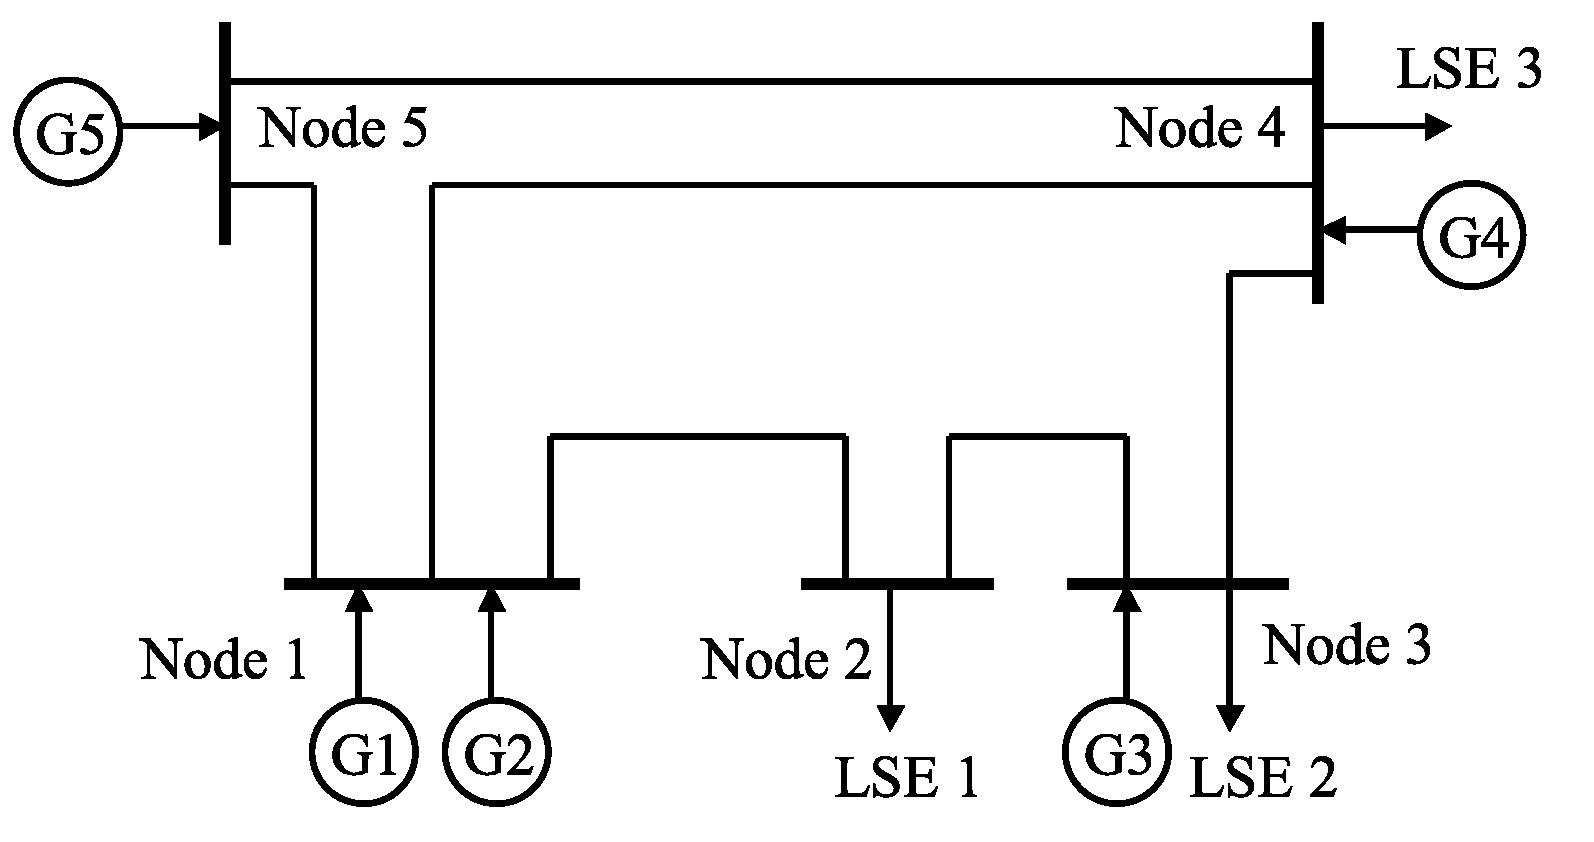
\includegraphics[totalheight = 8cm]{5Node.eps}
	\caption{A Five-Node Transmission Grid Configuration}
	\label{fig:5Node}
\end{figure}  


\begin{figure}
	\centering
		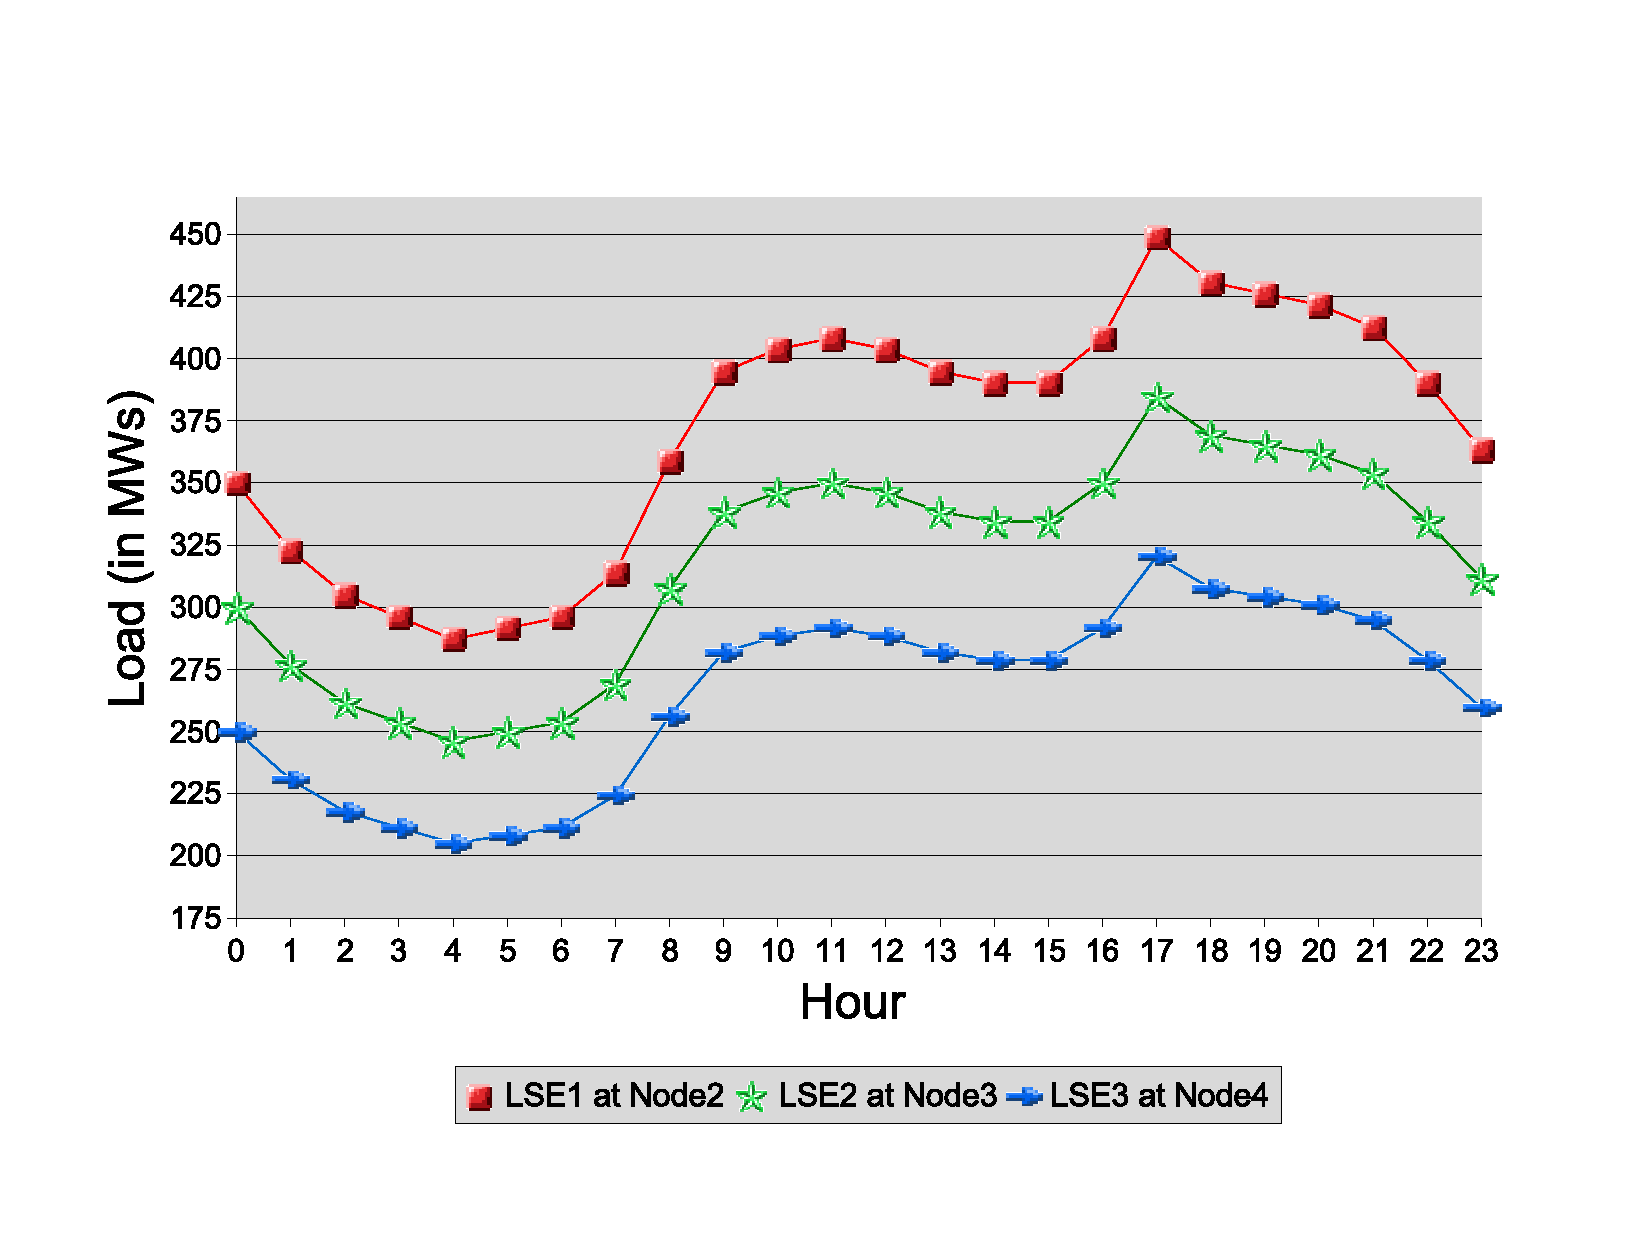
\includegraphics[totalheight = 10cm]{AMES.24HourLoad00-23.eps}
	\caption{24 Hour Load Distribution for the Dynamic 5-Node Test Case}
	\label{fig:24HourLoad.5Node}
\end{figure}
%%%%%%%%%%%%%%%%%%%%%%%%%%%%%%%%%%%%%%%%%%%%%%


\subsection{Treatment 1: Generators Report True Supply Data \label{5NodeCaseWithNoStrat} }

Suppose each Generator submits its true marginal cost function and true production limits into the Day-Ahead Market.  That is, suppose Generators do not report strategic supply offers. In this case, the augmented DC OPF problem solved by the ISO for each hour H involves the minimization of true Generator total variable cost (subject to a small voltage angle difference penalty) conditional on LSE loads, nodal balance constraints, true Generator upper and lower production limits, and upper and lower thermal limits on each branch of the transmission grid; compare Section~\ref{ISOConfig}.

     Tables~\ref{tab: 5Node.NoLearning.BranchFlows} and \ref{tab: 5Node.NoLearning.ProdsLMPsMinTVC} report outcomes in standard (SI) units obtained for this dynamic 5-node test case by means of QuadProgJ invoked through DCOPFJ.  These outcomes include optimized solution values for real power branch flows, production levels, LMPs (nodal balance constraint multipliers), and minimum total variable cost for 24 successive hours in the Day-Ahead Market.  

These outcomes reveal that branch congestion occurs between node 1 and node 2 (and only these nodes) in each of the 24 hours.  This can be verified by examining column $P_{12}$ in Table~\ref{tab: 5Node.NoLearning.BranchFlows}, which shows that the real power flow $P_{12}$ on branch $km=12$ is at its upper thermal limit (250 MWs) for each hour.  The direct consequence of this branch congestion is the occurrence of widespread LMP separation, i.e. the LMP values differ across all nodes for each hour.  This can be verified by examining output columns $\mbox{LMP}_1$-$\mbox{LMP}_5$ in Table \ref{tab: 5Node.NoLearning.ProdsLMPsMinTVC}.  

     Examining this LMP data more closely, it is seen that $LMP_{2}$ and $LMP_{3}$ (the LMPs for nodes 2 and 3) exhibit a sharp change in hour 17, increasing between hour 16 and hour 17 by about 100\%
and then dropping back to more normal levels in hour 18 and beyond.  Interestingly, this type of sudden spiking in LMP values is also observed empirically in MISO's Dynamic LMP Contour Map for real-time market prices, which is updated every five minutes; see, for example, Figure~\ref{fig:MISOLMP}.


%%%%%%%%%%%%%%%%%%%%%%%%%%%%%%%%%%%%%%%%%%%%%%%%%%%
\begin{figure}
	\centering
		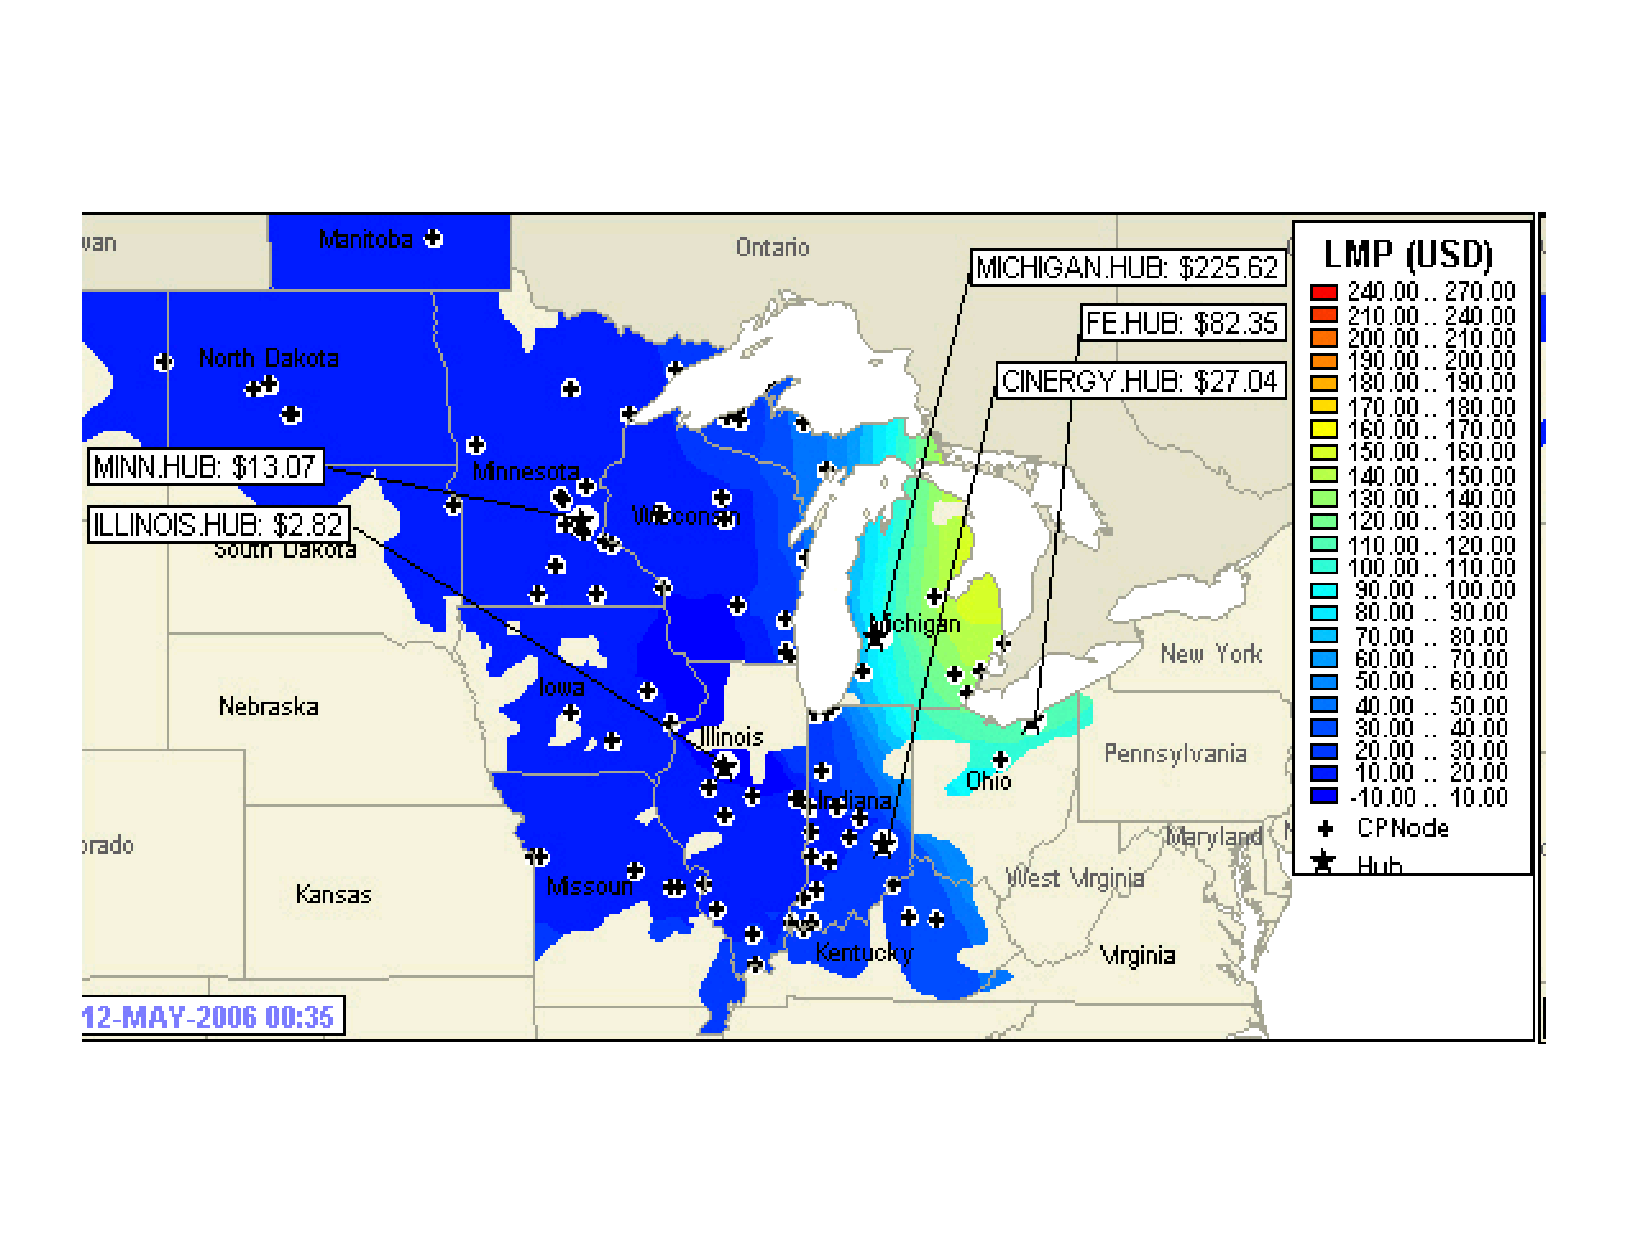
\includegraphics[totalheight = 8.5cm]{MISOLMP.MichiganCongestion.eps}
	\caption{LMP Separation and Spiking in the MISO Energy Region (Source: 
                Midwest ISO, http://www.midwestmarket.org/page/LMP\%20Contour\%20Map\%20\&\%20Data ) }
	\label{fig:MISOLMP}
\end{figure} 

%%%%%%%%%%%%%%%%%%%%%%%%%%%%%%%%%%%%%%%%%%%%%%%%555
     
     The rather dramatic LMP spiking in hour 17 can be traced to several factors. First, as seen in 
Figure~\ref{fig:24HourLoad.5Node}, the load profile for each LSE peaks at hour 17.  Second, when solving the DC OPF problem to meet the high load in hour 17, the ISO has to take into consideration the thermal limit constraining the flow of power on branch $km=12$ as well as the upper limit $\mbox{Cap}^U$ constraining the production of Generator 3.
Both of these constraints turn out to be binding in hour 17.  As seen in Table~\ref{tab: 5Node.NoLearning.BranchFlows}, the real power flow in branch $km=12$ is at its upper limit (250 MWs) for all 24 hours.  As seen in Table~\ref{tab: 5Node.NoLearning.ProdsLMPsMinTVC}, Generator 3 is dispatched in hour 17 at its upper production limit (520 MWs). 


Given the configuration of the transmission grid, to meet the hour 17 peak load the ISO is forced to back down (relative to hour 16) the less expensive production of Generators 1 and 2 and to use instead the more expensive production of the ``peaker" Generator 4.  After the peak hour 17, the load returns to lower levels.  The ISO is then able to schedule Generator 1 and Generator 2 at their more normal levels, with Generator 1 at its upper production limit, and to avoid scheduling any production from Generation 4; note from Table~\ref{tab: 5NodeInput} that Generator 4's minimum production level ($\mbox{Cap}^L$) is 0.  Furthermore, the LMPs drop back to their more normal levels after hour 17.

     These illustrative 5-node test case outcomes for 24 successive hours in the Day-Ahead Market raise intriguing economic issues concerning the operation of ISO-managed wholesale power markets in the presence of inequality constraints on branch flows and production levels.  The strong sensitivity of the optimized LMP and real power production values to changes in the set of binding (active) constraints is of particular interest.   

     Equally intriguing, however, is whether the Generators might learn to make use of the outcomes for any particular operating day D to change their reported supply offers for day D+1 and beyond. The next section considers this issue.

%%%%%%%%%%%%%%%%%%%%%%%%%%%%%%%%%%%%%%%%%%%%%%%%%%%%%%%%%%%%%%%%%%%%
%%%%%%%%%%%%%%%%%%%%%%%%%%%%%%%%%%%%%%%%%%%%%%%%%%%%%%%%%%%%%%%%%%%%

\subsection{Treatment 2: Generators Report Strategic Supply Offers \label{5NodeCaseWithStrat} }
  
Now suppose, in contrast to Treatment 1, that the Generators do not necessarily report their true marginal costs to the ISO for the Day-Ahead Market.  Rather, using the VRE stochastic reinforcement learning algorithm detailed in 
Section~\ref{TraderLearning}, with parameter values as specified in Table~\ref{tab: 5NodeInput.Learning}, each profit-seeking Generator learns over time which marginal cost function to report to the ISO based on the profits it has earned from previously reported functions.  
 
To control for random effects, outcomes for the learning treatment are reported below in the form of mean and standard deviation values obtained for twenty runs using the twenty different seed values reported in Table~\ref{tab: 5NodeInput.Learning}.%
        \footnote{Each Generator implements VRE learning by means of its own JReLM learning module, which must be initialized with a seed value for its pseudo-random number generator.  Each initial seed value reported in Table~\ref{tab: 5NodeInput.Learning} is used to generate five pseudo-random numbers, one for each Generator.  Each of these numbers is then used in turn as the initial seed value for the corresponding Generator's JReLM learning module.} 
      Across all 20 runs, 422 simulated trading days was the maximum time it took for all five Generators to ``converge" to a sharply peaked choice probability distribution in which a probability of 0.999 was assigned to a single supply offer.%
    \footnote{The \textit{mean\/} convergence time across the 20 runs was actually only 62 simulated trading days with an actual computing time of about 4.5 minutes.}   
       Consequently, all learning outcomes reported below are for day 422.  
       
For simplicity, each Generator $i$ selects supply offers from its action domain using VRE reinforcement learning with commonly specified values for the four learning parameters $\{q(0),C, r,e\}$; cf.\ Section~\ref{TraderLearning}.  In addition, to ensure equal cardinalities and similar densities, each Generator $i$'s action domain $AD_i$ is constructed using commonly specified values for the six action-domain parameters $\{M1,M2,M3,\mbox{RIMax}^L,\mbox{RIMax}^U,SS\}$; cf.\ the detailed discussion in Appendix.  These parameter value specifications are listed in Table~\ref{tab: 5NodeInput.Learning}.  
       
Table~\ref{tab: 5Node.Learning.BranchFlows} provides detailed numerical solution values (means and standard deviations) for branch flows on day 422.  Recalling that the thermal limit on branch $km=12$ is 250MWs, note that congestion occurs on branch $km=12$ in the peak hour 17 (and for several hours thereafter) in all 20 runs.  Moreover, although 
the \textit{mean\/} flow on branch $km=12$ is slightly below the thermal limit in other hours, in fact this branch is congested during all 24 hours of day 422 in all but three of the twenty runs.  Moreover, no other branch is ever congested.  These findings are similar to  the no-learning treatment, in which branch $km=12$ (and only this branch) was found to be persistently congested.   

Tables \ref{tab: 5Node.Learning.Prods} and \ref{tab: 5Node.Learning.LMPs} provide detailed numerical solution values (means and standard deviations) for real power production levels and LMPs, respectively, on day 422.  
Table~\ref{tab: 5Node.Learning.ReportedCostCoeffs} gives the ordinate coefficient $a^R$ and slope coefficient $b^R$ for the (linear) marginal cost function reported to the ISO on Day 422 by each of the five Generators in each of the twenty runs.  In the following discussion we highlight various aspects of these outcomes that differ significantly from the corresponding outcomes presented for the no-learning treatment in Section~\ref{5NodeCaseWithNoStrat}.

Figure \ref{fig:Prods} displays the (mean) solution values obtained for production for each of the 24 hours on day 422, along with the corresponding solution values obtained for day 422 in the absence of Generator learning.%
    \footnote{Given the stationarity of the daily load profiles and the Generators' cost functions and production limits, and the absence of system disturbances, in the no-learning treatment the 24-hour outcomes obtained for any one day are the same as for any other day.}   
     In the no-learning treatment, note that the ``peaker" (high cost) Generator 4 is only dispatched to produce energy at the peak load hour 17.  In the learning treatment, however, Generator 4 is able to use strategic supply offers to ensure it is dispatched at approximately its upper production limit (200MWs) throughout each hour of the day.  
Also, in the no-learning treatment the ``cheap'' Generator 5 is regularly dispatched at a high production level during each hour of the day, but in the learning treatment it is backed way down because its strategic supply offers make it appear to be a relatively more expensive Generator.  


%%%%%%%%%%%%%%%%%%%%%%%%%%%%%%%%%%%%%%%%%%%%%%%%%%%
\begin{figure}
	\centering
		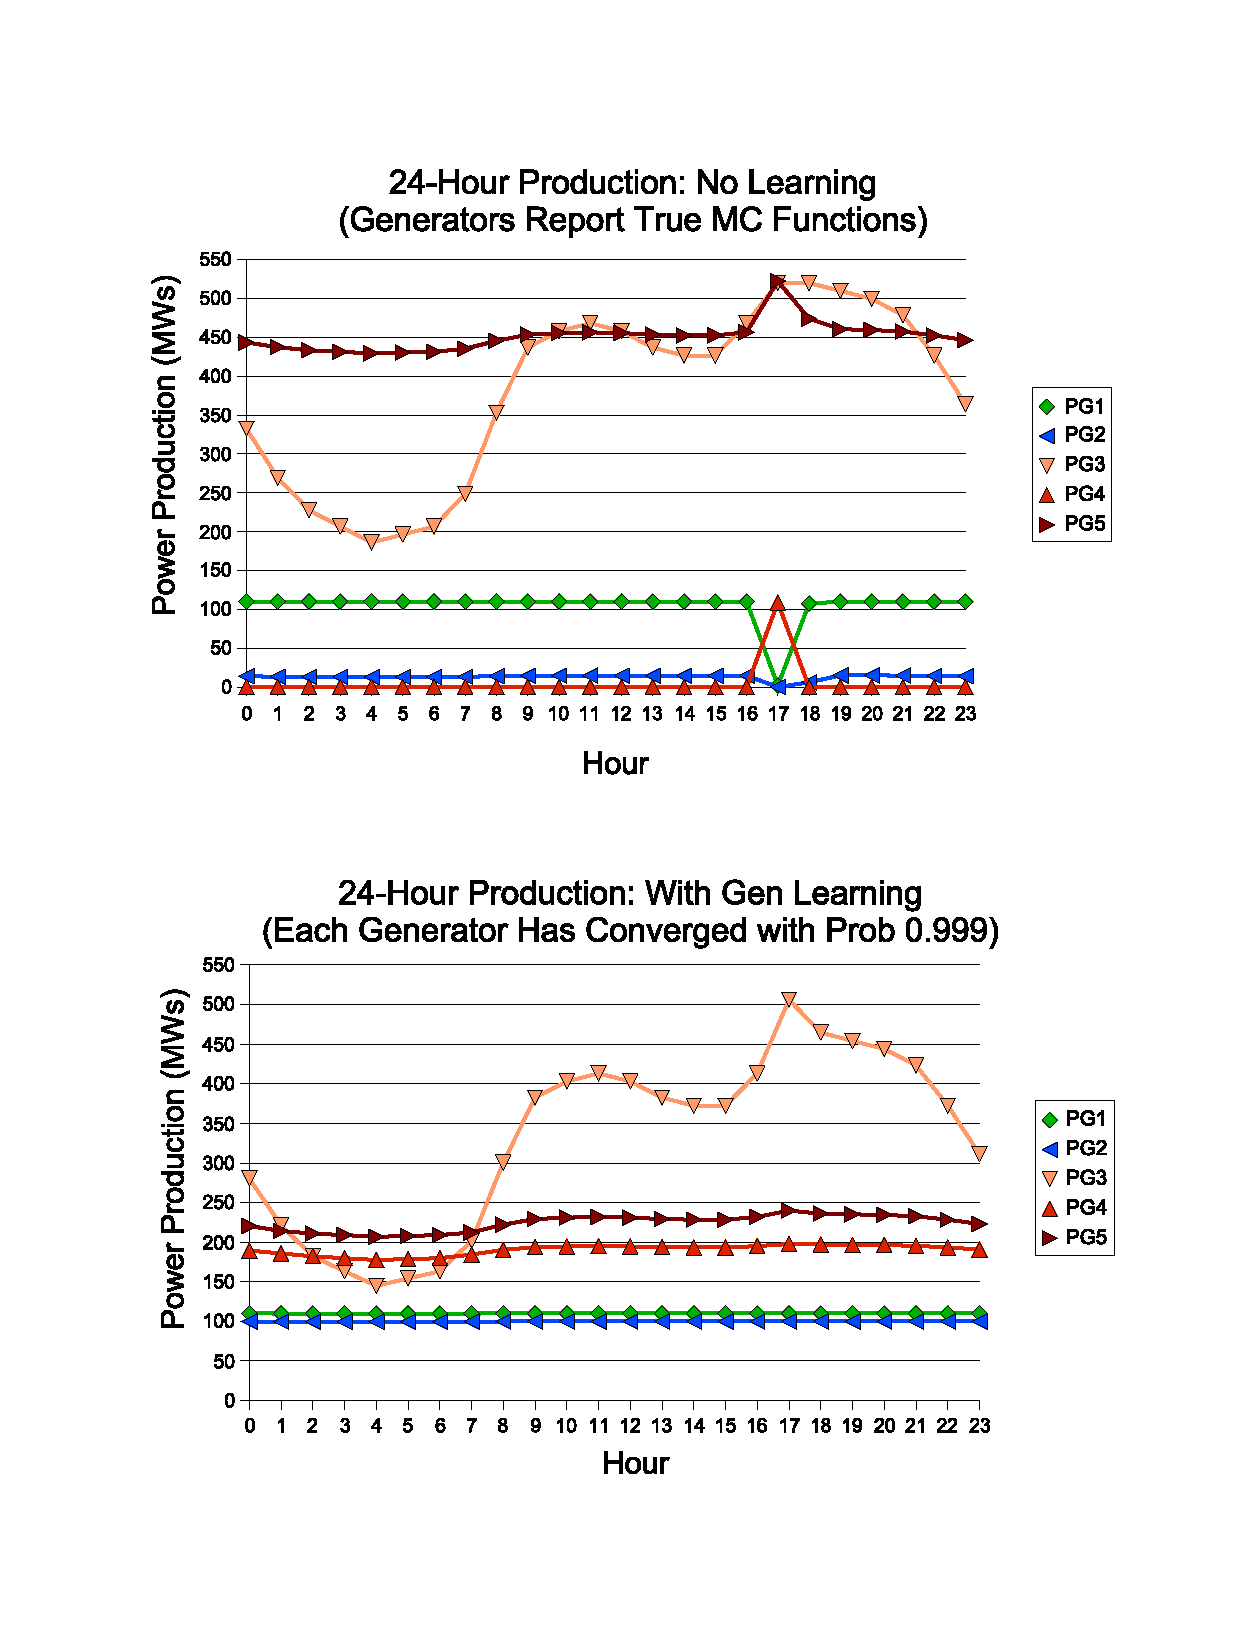
\includegraphics[totalheight = 20cm]{AMES.Results.Prods.eps}
	\caption{Dynamic 5-Node Test Case Solution Values for 24-Hour Real Power Production Levels (Day 422) -- Generator Learning Compared with No Learning}
	\label{fig:Prods}
\end{figure} 

%%%%%%%%%%%%%%%%%%%%%%%%%%%%%%%%%%

This heavier reliance on costlier generation in the learning treatment substantially increases the total variable cost of operation.  Indeed, as seen in Figure \ref{fig:CompareMinTVC}, the minimum total variable cost of operation under the learning treatment is roughly three times higher than under the no-learning treatment.



%%%%%%%%%%%%%%%%%%%%%%%%%%%%%%%%%%%%%%%%%%%%%%%5
\begin{figure}
	\centering
		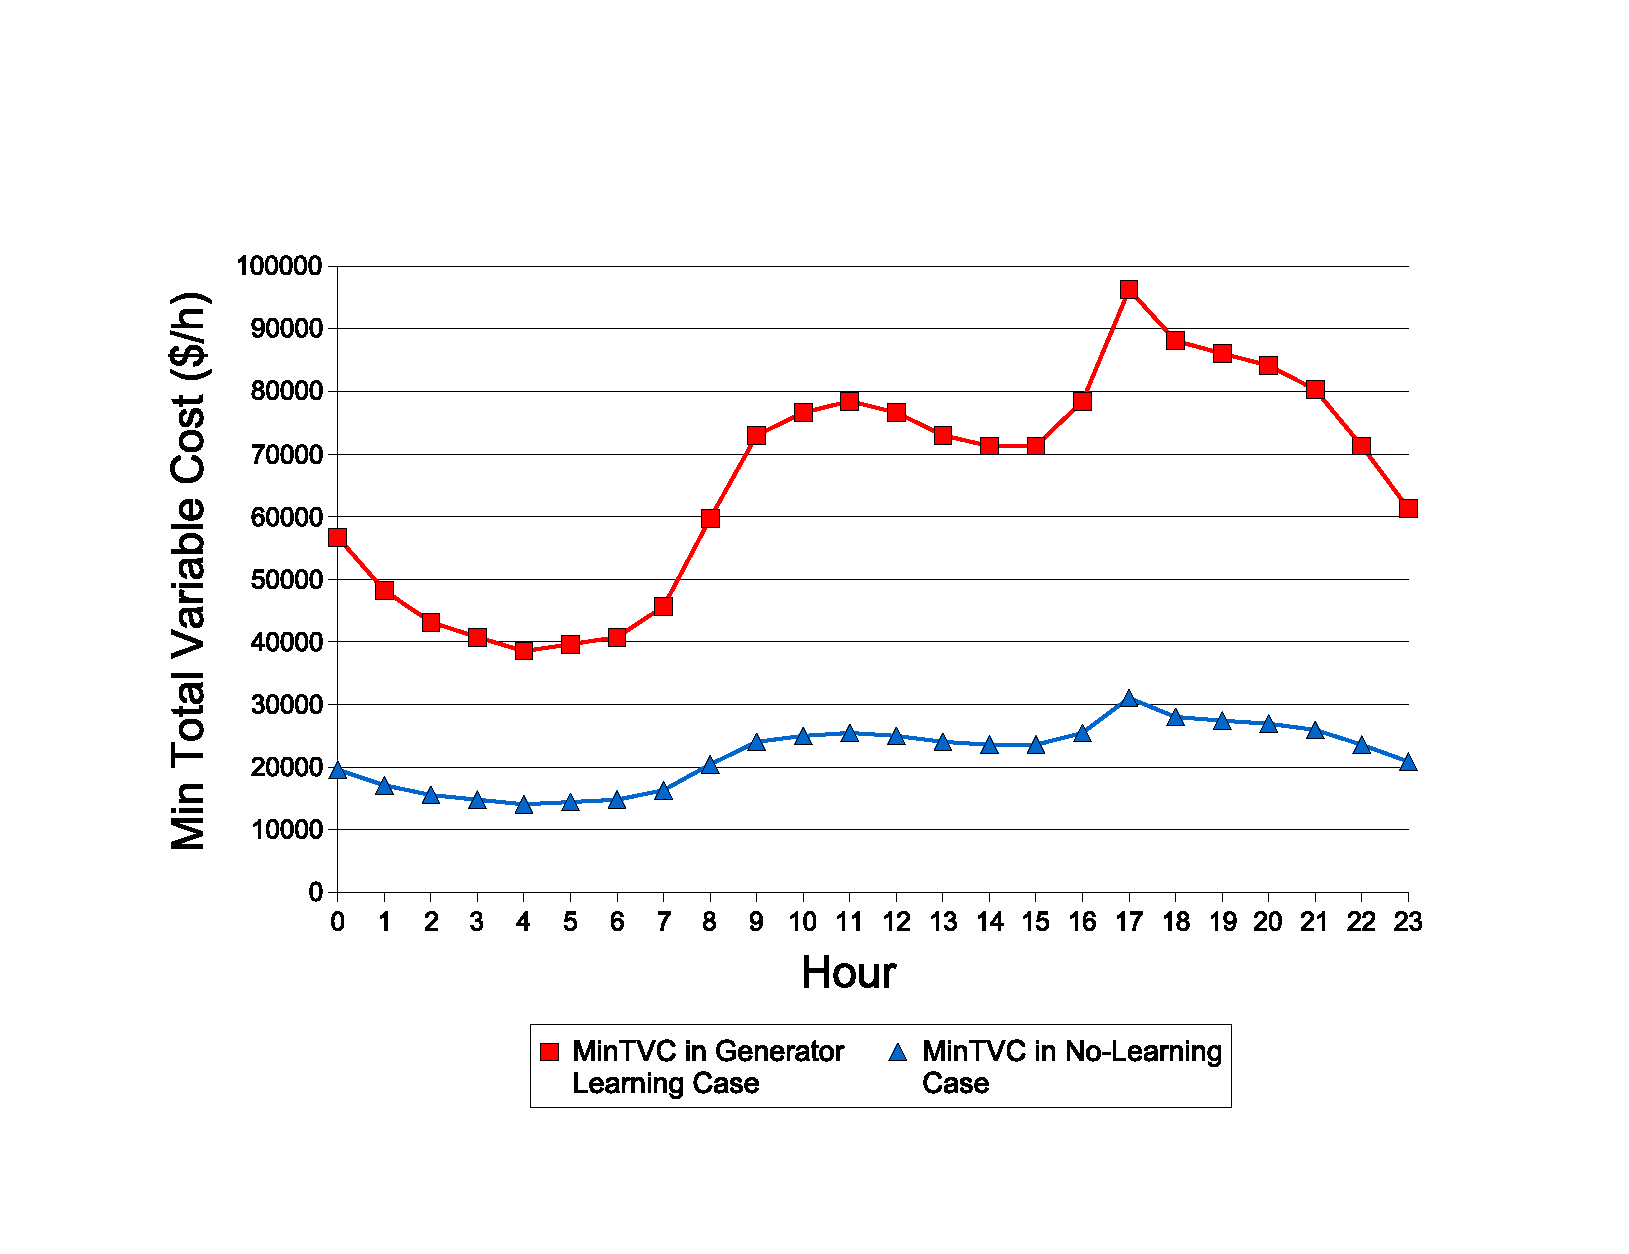
\includegraphics[totalheight = 10cm]{AMES.Results.CompareMinTVC.eps}
	\caption{Dynamic 5-Node Test Case Solution Values for 24-Hour Minimum Total Variable Cost (Day 422) -- Generator Learning Compared with No Learning }
	\label{fig:CompareMinTVC}
\end{figure} 
%%%%%%%%%%%%%%%%%%%%%%%%%%%%%%%%%%%%%%%%%%%%%%%%%%%%%%


Figure \ref{fig:LMPs} graphically depicts the 24-hour (mean) LMP solution values for the learning treatment along with the 24-hour LMP solution values for the no-learning treatment.  Interestingly, although the LMPs for the learning treatment are considerably higher than the LMPs for the no-learning treatment, they are also less volatile around the peak load hour 17.  Consequently, the ISO is not able to use the appearance of price spikes in peak load hours to detect the considerable exercise of market power by the learning Generators.  Rather, some form of direct auditing of the Generators' cost attributes would seem to be required.  

%%%%%%%%%%%%%%%%%%%%%%%%%%%%%%%%%%%%%%%%

\begin{figure}
	\centering
		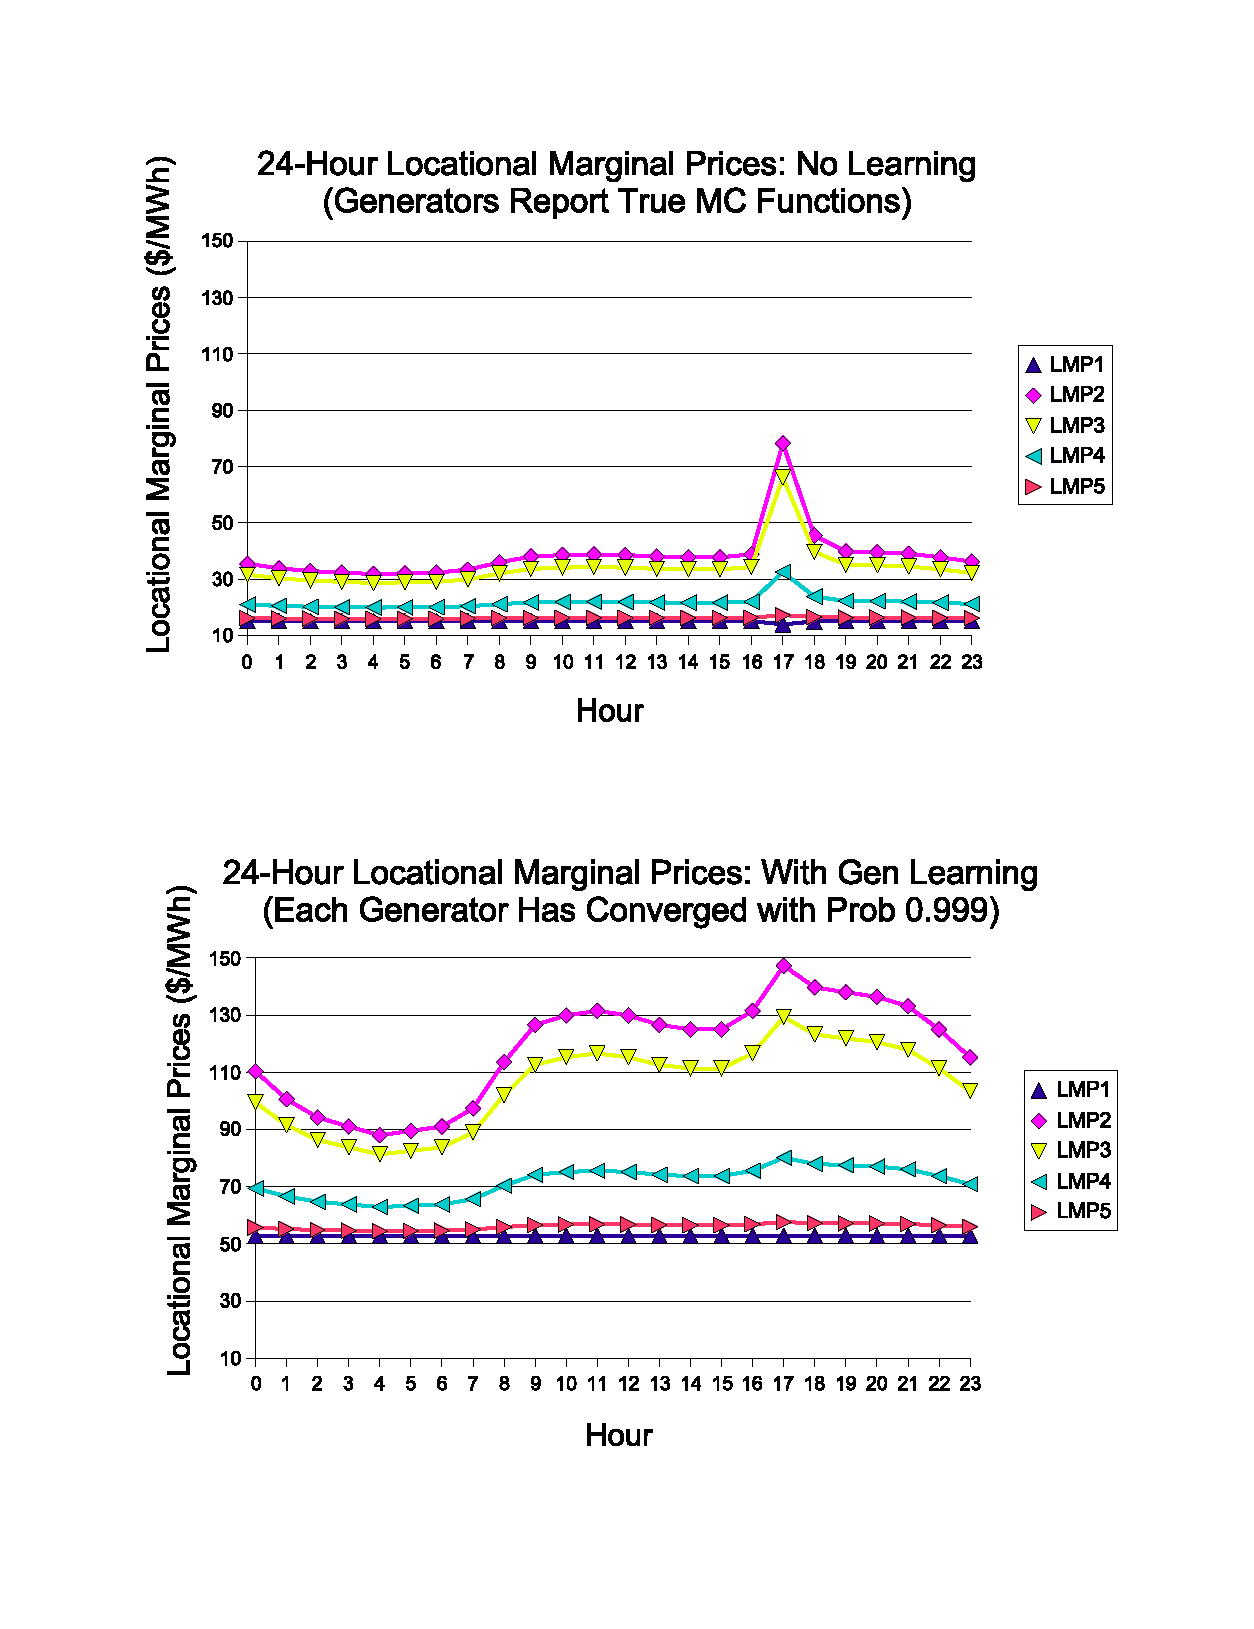
\includegraphics[totalheight = 20cm]{AMES.Results.LMPs.eps}
	\caption{Dynamic 5-Node Test Case Solution Values for 24-Hour LMPs (Day 422) -- Generator Learning Compared with No Learning}
	\label{fig:LMPs}
\end{figure} 
%%%%%%%%%%%%%%%%%%%%%%%%%%%%%%%%%%%%%%%%%%
 
Figure \ref{fig:MCs} displays the (mean) marginal cost functions that the five Generators report to the ISO on day 422, along with their true marginal cost functions.  Despite the absence of any explicit collusion, all five Generators have learned to report higher-than-true marginal cost functions with respect to both ordinate and slope.  In the case of Generators 3 and 5, the two largest generating units, the increase is substantial; these two Generators quickly learn to report a marginal cost function that is near or at the highest level permitted in their action domains.%
         \footnote{More precisely, the lower and upper range-index values implied by these Generators' reported marginal cost curves typically converge with rapidity to values that are near or at their highest permitted range-index
levels $\mbox{RIMax}^L=0.75$ and $\mbox{RIMax}^U = 0.75$; cf.~Table~\ref{tab: 5NodeInput.Learning}.} 
  Clearly the core aspects of the WPMP market design currently captured in the AMES framework do not provide sufficient mechanisms to prevent Generators from exercising substantial market power through strategic reporting of supply offers. 

%%%%%%%%%%%%%%%%%%%%%%%%%%%%%%%%%%%%%%%%%%%%%%%%%5

\begin{figure}
	\centering
		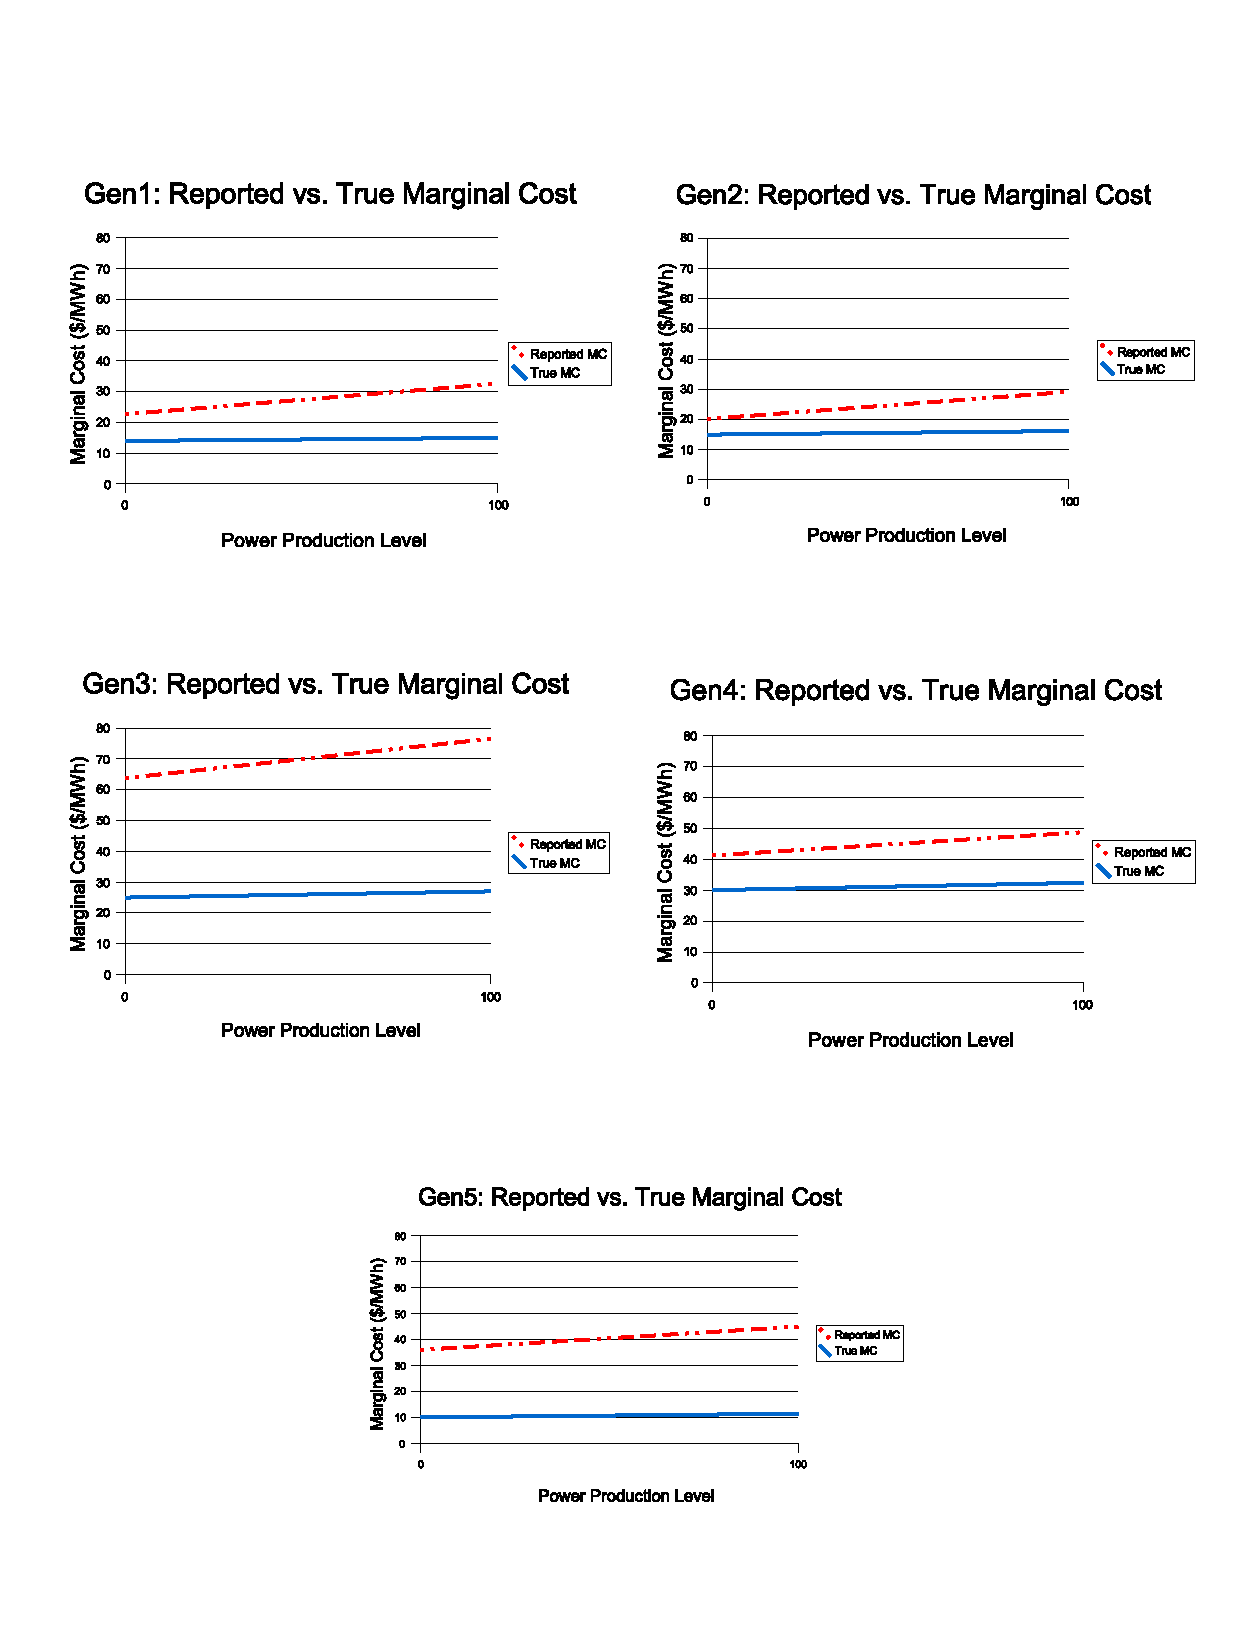
\includegraphics[totalheight = 20cm]{AMES.Results.MCs.eps}
	\caption{Dynamic 5-Node Test Case -- Mean Reported Marginal Cost Function Versus True Marginal Cost Function for Each Generator (Day 422)}
	\label{fig:MCs}
\end{figure} 

%%%%%%%%%%%%%%%%%%%%%%%%%%%%%%%%%%%%%%%%%%%%%%%

These findings can be compared with the findings of Wolfram~(1999), who determined empirically that the (pre-NETA) uniform-price auction design in effect for the UK wholesale power market at the time of her study provided incentives for generators to raise prices above costs.  In addition, Mount~(2000) uses a simple analytical framework to show how generators facing normally-distributed demand in a wholesale power market operated as a uniform-price auction have an incentive to submit supply offers that far exceed their true costs.
The AMES Day-Ahead Market collapses to a uniform-price auction only in the absence of transmission congestion; LMP separation occurs when any branch is congested.  However, using simple reinforcement learning with no explicit collusion, the AMES Generators quickly co-learn how to submit supply offers that result in substantial market power whether or not LMP separation occurs.

%%%%%%%%%%%%%%%%%%%%%%%%%%%%%%%%%%%%%%%%%%%%%%%%%%%%%%%%%%%%%%%%%%%%
%%%%%%%%%%%%%%%%%%%%%%%%%%%%%%%%%%%%%%%%%%%%%%%%%%%%%%%%%%%%%%%%%%%%
%%%%%%%%%%  NEW SECTION %%%%%%%%%%%%%%%%%%%%%%%%%%%%%%%%%%%%%%%%%%%%
%%%%%%%%%%%%%%%%%%%%%%%%%%%%%%%%%%%%%%%%%%%%%%%%%%%%%%%%%%%%%%%%%%%%

\section{Concluding Remarks \label{Conclusion}}


The North American power transmission grid has been called ``the largest and most complex machine in the world" (Amin, 2004, p.~31).  An extraordinary experiment is under way to see whether the physical operation of this complex machine can be successfully married with a restructured commercial architecture encouraging increased reliance on demand and supply forces.  Smart electrical devices permitting more distributed physical control of the grid are being introduced along with market designs permitting more decentralized pricing and allocation mechanisms, a trend one commentator has called ``electricity's third great revolution" (Mazza, 2003).

Stakeholders, policy makers, and researchers all clearly recognize the critical need for this experiment to succeed (FERC, 2007).  Nevertheless, the issues raised by this experiment are extremely challenging.  How to analyze the potential dynamic performance of a system comprising multiple distributed entities, some physical and some human, all with finite information and computational capabilities?  How to properly take into account the stability limits of physical components as well as the strategic behaviors of human participants responding to the incentives deliberately or inadvertently presented by system design features?

Agent-based modeling tools have been specifically developed to handle these types of complexities, hence it is
not surprising to find agent-based researchers actively involved in this electricity restructuring movement.  As detailed by Davidson and McArthur~(2005) and by Widergren et al.~(2006), multi-agent systems are attracting significant research interest for power system applications.  Indeed, the \textit{IEEE Working Group on Multi-Agent Systems in Power Engineering\/} is charged with exploring the benefits, applications, and advanced functionality that can be provided for power systems through agent technology. The members of this IEEE MAS Working Group include economists as well as engineers, and academics as well as industry stakeholders.  

In this study we explore the potential usefulness of agent-based tools for investigating the efficiency and reliability of the Wholesale Power Market Platform (WPMP), a market design proposed by the U.S. Federal Energy Regulatory Commission for common adoption by all U.S. wholesale power markets (FERC, 2003).  We first describe a newly developed agent-based computational laboratory -- the AMES framework -- that models a wholesale power market operating in accordance with core WPMP features over a realistically rendered transmission grid subject to congestion effects.  Using a dynamic 5-node test case for concrete illustration, we then explore the extent to which these core WPMP features permit and even encourage the exercise of market power by Generators through strategic reporting of supply offers.  

More precisely, in the dynamic 5-node test case the AMES ISO does not know the AMES Generators' true cost attributes.  Rather, in each operating day D, the AMES ISO must formulate its DC-OPF problem for each hour of the Day-Ahead Market for day D+1 based on the cost attributes reported to it by the Generators. The profit-seeking Generators learn over time what cost attributes to report to the ISO using a simple reinforcement learning algorithm based on past profit outcomes. 

As seen in Section~\ref{5NodeTestCase}, in a typical run the Generators converge within 62 simulated trading days to supply offer selections for which their reported marginal cost functions are uniformly higher than their true marginal cost functions, in some cases substantially higher, despite the absence of any explicit collusion.  The resulting ``optimal" DC-OPF solutions determined by the AMES ISO appear to have desirable properties, e.g. low LMP volatility during peak load hours and congestion on only one branch.  In fact, however, total variable costs of operation are roughly three times higher than they would have been had the Generators reported their true cost attributes.  As captured in the current AMES framework, the core WPMP design features do not prevent the considerable exercise of market power by Generators.


As detailed in Section~\ref{AMESOverview}, the AMES framework needs to be further extended to incorporate additional key aspects of the WPMP design that could significantly impact the efficiency and reliability of market operations. Moreover, initial conditions and parameter specifications need to be more carefully calibrated to match real-world conditions.  Nevertheless, we believe the preliminary findings reported in this study suggest the great potential of agent-based computational models to help ensure a successful restructuring of the electric power industry through intensive sensitivity experiments.


%%%%%%%%%%%%%%%%%%%%%%%%%%%%%%%%%%%%%%%%%%%%%%%%%%

\bigskip
\bigskip
\noindent \textbf{\Large References}

\smallskip
\begin{description}

\item Amin, Massoud~(2004). Balancing market priorities with security issues,
{\it IEEE Power and Energy Magazine\/}, July/August, pp.~30-38.

\item Axelrod, Robert, and Tesfatsion, Leigh~(2007).  A guide for newcomers to agent-based modeling in the social 
sciences.  In Leigh Tesfatsion and Kenneth L. Judd, \textit{op. cit.\/}.  Available:
http://www.econ.iastate.edu/tesfatsi/abmread.htm 

\item Barreteau, Olivier~(2003). Our companion modeling approach, \textit{Journal of Artificial 
Societies and Social Simulation\/} 6(1) (electronic), http://jasss.soc.surrey.ac.uk/6/2/1.html 

\item Borenstein, Soren~(2002). The trouble with electricity markets: Understanding
California's restructuring disaster, {\it J.\ Econ.\ Perspectives\/}
16(1), 191-211.

\item Bower, John, and Bunn, Derek ~(2001). Experimental analysis of the efficiency of uniform-price versus discriminatory auctions in the England and Wales electricity market, {\it Journal of Economic Dynamics and Control\/} 25(3-4), 561-592.

\item Cain, Mary B., and Alvarado, Fernando L.~(2004).  Implications of cost and bid format on electricity market studies: Linear versus quadratic costs, \textit{Proceedings\/}, Large Engineering Systems Conference on Power Engineering, Halifax, Canada, July.

\item Conzelmann, Guenter, North, Michael J., Boyd, Gale A., Cirillo, Richard R., Koritarov, Vladimir, Macal, Charles M., Thimmapuram, Prakash R., and Veselka, Thomas D.~(2004). Simulating strategic market behavior using an agent-based modeling approach, \textit{Proceedings}, 6th IAEE European Conference, Zurich, Switzerland.

\item Davidson, Euan M., and McArthur, Stephen D.~J.~(2005).  Concepts and approaches in multi-agent 
systems for power applications, \textit{Proceedings\/}, Intelligent System Applications in Power (ISAP) 
Conference, Washington D.C., November, pp.~391-395.

\item Erev, Ido, and Roth, Alvin E.~(1998).  Predicting how people play games with unique
mixed-strategy equilibria, {\it American Economic Review\/} 88, 848-881.

\item FERC~(2003). {\it Notice of White Paper\/}, U.S. Federal Energy Regulatory
Commission, 4/28.

\item FERC~(2007). Report to Congress on competition in the wholesale and retail markets for electric energy, 
U.S. Federal Energy Regulatory Commission, May.  Available:
http://www.ferc.gov/legal/maj-ord-reg/fed-sta/ene-pol-act/epact-final-rpt.pdf

\item Gieseler, Charles~J.~(2005).  A Java reinforcement learning module for the Repast toolkit:
Facilitating study and experimentation with reinforcement learning in social science multi-agent
simulations, M.S.\ Thesis, Computer Science, Iowa
State University, November.

\item ISO-NE~(2007). Home Page, ISO New England, Inc. 
Available: http://www.iso-ne.com/smd/

\item Joskow, Paul (2006).  Markets for power in the United States: An interim assessment, \textit{Energy Journal\/}, 
Vol.\ 27(1), 1-36.

\item
Kirschen, Daniel, and Strbac, Goran~(2004). \textit{Fundamentals of Power System Economics\/}, 
John Wiley \& Sons, Inc., New York, NY.

\item
Koesrindartoto, Deddy~(2002).  A discrete double auction with artificial adaptive
agents:  A case study of an electricity market using a double-auction
simulator, Economics Working Paper No.~02005, Department of Economics, Iowa
State University, Ames, IA.  Available: http://deddy.agenbased.net/res.html

\item Koesrindartoto, Deddy, Sun, Junjie, and Tesfatsion, Leigh~(2005).  An agent-based computational
laboratory for testing the economic reliability of wholesale power market designs, 
{\it Proceedings\/}, Vol.~1, IEEE Power Engineering Society General Meeting, San Francisco, CA,
June, 931-936.

\item Lally, John~(2002). Financial transmission rights: Auction example, Section 6, M-06 
Financial Transmission Right Draft 01-10-02, ISO New England, Inc., January.

\item Mazza, Patrick (2003).  The smart energy network: Electricity's third great revolution, 
Report prepared for Climate Solutions, Olympia, WA, June.  Accessible:\\ 
http://www.climatesolutions.org/pubs/pdfs/SmartEnergy.pdf

\item McCalley, James, Ryan, Sarah, Sapp, Stephen, and Tesfatsion, Leigh~(2005).  Decision models 
for bulk energy transportation networks, Division of Electrical and Communication Systems, 
National Science Foundation Grant No. 0527460, 3/15/05 - 3/14/08.

\item MISO~(2007), Home Page, Midwest ISO, Inc..  Available:
http://www.midwestiso.org/

\item Mount, Timothy D.~(2000).  Strategic behavior in spot markets for electricity when load is stochastic. 
\textit{Proceedings\/}, 33rd Hawaii International Conference on Systems Science.

\item Nicolaisen, James, Petrov, Valentin, and Tesfatsion, Leigh~(2001).  Market power and
efficiency in a computational electricity market with discriminatory
double-auction pricing, {\it IEEE Transactions on Evolutionary Computation\/}
5(5), 504-523.

\item Roth, Alvin E., and Erev, Ido~(1995).  Learning in extensive form games:
Experimental data and simple dynamic models in the intermediate term,
{\it Games and Econ.\ Behavior\/} 8, 164-212.

\item Shahidehpour, Mohammad, Yamin, Hatim, and Li, Zuyi~(2002).  \textit{Market Operations in Electric Power Systems\/}, IEEE/Wiley-Interscience, John Wiley \& Sons, Inc., NY.

\item Sun, Junjie (2006).  U.S. financial transmission rights: Theory and practice, Economics
Working Paper No.~05008, Economics Department, Iowa State University.

\item Sun, Junjie, and Tesfatsion, Leigh~(2007a). DC optimal power flow formulation and solution using QuadProgJ,  Economics Working Paper No.~06014, Economics Department, Iowa State University, Revised: July.\\
Available: http://www.econ.iastate.edu/tesfatsi/DC-OPF.JSLT.pdf

\item Sun, Junjie, and Tesfatsion, Leigh~(2007b). Open-source software for power industry research, teaching, and training: A DC-OPF illustration, \textit{Proceedings\/}, IEEE Power Engineering Society General Meeting, Tampa, Florida, June.

\item Tesfatsion, Leigh~(2007a). \textit{ACE Research Area: Restructured Electricity Markets\/}, Website available at http://www.econ.iastate.edu/tesfatsi/aelect.htm

\item Tesfatsion, Leigh~(2007b). \textit{Website on Agent-based Computational Economics (ACE)\/}, Website available at: http://www.econ.iastate.edu/tesfatsi/ace.htm

\item Tesfatsion, Leigh~(2007c). \textit{The AMES Market Package (Java): A Free Open-Source Test Bed for the Agent-based Modeling of Electricity Systems\/}, Website available at:\\
http://www.econ.iastate.edu/tesfatsi/AMESMarketHome.htm

\item Tesfatsion, Leigh~(2007d). \textit{Verification and Validation of Agent-Based 
Computational Models\/}, Website available at http://www.econ.iastate.edu/tesfatsi/EmpValid.htm

\item Tesfatsion, Leigh~(2007e). \textit{RepastJ: A Software Toolkit for Agent-Based Social Science Modeling\/}, 
Website available at http://www.econ.iastate.edu/tesfatsi/repastsg.htm

\item Tesfatsion, Leigh~(2007f). \textit{General Software and Toolkits: Agent-Based Computational Economics\/}, 
Website available at http://www.econ.iastate.edu/tesfatsi/acecode.htm

\item Tesfatsion, Leigh, and Judd, Kenneth L., eds.~(2006). \textit{Handbook of 
Computational Economics, Vol.~2: Agent-Based Computational Economics\/}, Handbooks in 
Economics Series, North-Holland, Elsevier, Amsterdam, the Netherlands.

\item Weisfeld, Matt~(2003). \textit{The Object-Oriented Thought Process\/}, Second Edition, SAMS, MacMillan USA, Indiana.

\item Widergren, Steven, Roop, Joseph M., Guttromson, R. T., and Huang, Z.~(2004). Simulating the dynamic coupling of market and physical system operations, \textit{Proceedings\/}, 2004 IEEE PES General Meeting, Denver, Colorado.\\
Available: http://gridwise.pnl.gov/docs/pnnl40415.pdf

\item Widergren, Steven, Sun, Junjie, and Tesfatsion, Leigh~(2006).  Market design test environments, 
\textit{Proceedings\/}, IEEE Power Engineering Society General Meeting, Montreal, June.

\item Wilson, Robert~(2002).  Architecture of power markets, \textit{Econometrica\/}, Vol. 70, No. 4, July, 1299-1340.

\item Windrum, Paul, Fagiolo, Giorgio, Windrum, Paul, and Moneta, Alessio~(2007). Empirical validation of 
agent-based models: Alternatives and prospects. \textit{J.~of Artificial Societies and Social Simulation\/},
10(2,8).~Available: http://jasss.soc.surrey.ac.uk/10/2/8.html


\item Wolfram, Catherine D.~(1999).  Electriciy markets: Should the rest of the world adopt the United Kingdom's reforms?, \textit{Regulation\/} 22(4), 48-53.

\item Veit, Daniel, Weidlich, Anke, Yao, Jian, and Oren, Shmuel (2006).  Simulating the dynamics in two-settlement electricity markets via an agent-based approach, \textit{International Journal of Management Science and Engineering Management\/}, 1(2), 83-97. Working paper available at:  http://www.ieor.berkeley.edu/~jyao/pubs/yao-MS06.pdf

\pagebreak

\end{description}


%%%%%%%%%%%%%%%%%%%%%%%%%%%%%%%%%%%%%%%%%%%%%%%%%%%%%%%%%%%%%%
%%%%%%%%%%%%%%%%%%%%%%%%%%%%%%%%%%%%%%%%%%%%%%%%%%%%%%%%%%%%%%

\bigskip
\noindent
\textbf{\Large Appendix: Construction of Generator Action Domains}

\bigskip
\noindent
\textbf{\large A.1 Overview}

\medskip
\noindent
As detailed in 
Section~\ref{TraderLearning}, at the beginning of each day D each
AMES Generator $i$ uses a variant of a well known Roth-Erev reinforcement learning algorithm to choose a 
supply offer $s^R_i$ to report to the AMES ISO for each hour H of the day D+1  Day-Ahead Market.  Each supply 
offer $s^R_i$ takes the form of a reported marginal cost function 
\begin{equation} \label{AppReportedMC}
              \mbox{MC}^R_i(p) = a^R_i + 2b^R_i p  
\end{equation}

\smallskip
\noindent
defined over a reported feasible production interval
          \begin{equation}  \label{AppReportedPI}
     \mbox{Cap}^{RL}_i ~\le  ~ p \le ~~ \mbox{Cap}^{RU}_i
          \end{equation}
Here $a^R_i$ and $b^R_i$ are Generator $i$'s reported cost coefficients, p denotes Generator $i$'s hourly real-power production level, and $\mbox{Cap}^{RL}_i$ and $\mbox{Cap}^{RU}_i$ are Generator $i$'s reported lower and upper real-power production limits.

Each AMES Generator $i$ chooses its supply offers $s^R_i$ from an action domain $AD_i$ with finite positive cardinality
$M_i$.  A key issue is how to construct this action domain in a manner that is both empirically sensible and computationally practical.  Empirical sensibility suggests that, unless the modeler has information to the contrary, the action domain $AD_i$ should provide Generator $i$ with the flexibility to choose from among a wide range of possible supply offers, and that this degree of flexibility should be roughly similar across the Generators.  Computational practicality suggests that the number of  supply offers included in $AD_i$ should not be unduly large.

In keeping with these modeling goals, the action domain $AD_i$ for each AMES Generator $i$ is constructed under 
five simplifying assumptions. 
       First, we assume that Generator $i$ only reports upward-sloping marginal cost functions (\ref{AppReportedMC}),
i.e., $b^R_i > 0$.%
         \footnote{In the MISO and ISO-NE, reported supply functions are required to be non-decreasing.}  
     Second, we assume that Generator $i$ only reports non-trivial feasible production intervals (\ref{AppReportedPI}), i.e., $\mbox{Cap}^{RL}_i  <  \mbox{Cap}^{RU}_i$.     
     Third, we assume that Generator $i$ only reports marginal cost curves that lie on or above Generator $i$'s true marginal cost curve over the range of their accompanying reported production intervals. 
       Fourth, we assume that Generator $i$ always reports its true lower production limit.%     
    \footnote{As explained in footnote~\ref{FirmLowerProdLimits}, the Generators' reported lower production limits are treated as firm by the AMES ISO.  Since the current version of AMES lacks market power mitigation rules, the AMES Generators could ensure themselves arbitrarily high profits if they were permited to \textit{report\/} arbitrarily high lower production limits into the Day-Ahead Market. For this reason, it is assumed in the current study that the AMES Generators are closely monitored by the AMES ISO with regard to these lower production limits, ensuring that they always report their true lower limits. In the actual MISO and ISO-NE energy markets, generators are requested to report their true lower and upper production limits, but it is not clear from the MISO and ISO-NE business practices manuals just how closely generators are actually monitored to ensure compliance.\label{ProdLimCompliance}}
    Fifth, we assume that Generator $i$ always reports an upper production limit that is less than or equal to its true upper production limit.     

We show below that, given any positive value for a \textit{slope-start\/} parameter $SS_i$, we can construct 
an $M_i\times 3$ matrix whose rows constitute $M_i$ admissible supply offers in percentage form that map 
uniquely into $M_i$ reported supply offers $s^R_i$ satisfying the five simplifying assumptions above.  This matrix is parameterized by three density-control parameters $M1_i$, $M2_i$ and $M3_i$ (with $M1_i\times M2_i \times M3_i = M_i$) and three range-index parameters $\mbox{RIMax}^L_i$, $\mbox{RIMax}^U_i$, and $\mbox{RIMin}^C_i$.%
     \footnote{As clarified below in Sections A.2 through A.4, the range-index parameters $\mbox{RIMax}^L_i$  
and $\mbox{RIMax}^U_i$ in $[0,1)$ can be related to the standard ``Lerner Index" used in industrial organization studies as an indicator of market power.  The range-index parameter $\mbox{RIMin}^C_i$ in $(0,1]$ governs capacity withholding, hence it also relates to market power.} 
     If the parameters $(M1_i,M2_i,M3_i,\mbox{RIMax}^L_i,\mbox{RIMax}^U_i,\mbox{RIMin}^C_i,SS_i)$ are set identically for each Generator $i$, and the above matrix construction is applied for each Generator $i$, then the result is a collection of Generator-specific action domains that have equal cardinalities and whose supply offer elements $s^R$ provide similar densities of coverage of the regions lying above the Generators' true marginal cost curves.  

%%%%%%%%%%%%%%%%%%%%%%%%%%%%%%%%%%%%%%%% Appendix Sub-section %%%%%%%%%%%%%%%%%%%%%%%%%%%%%%%%%%%%%%%%%

\bigskip
\noindent
\textbf{\large A.2 Percentage Representation of Supply Offers}

\medskip
\noindent

 
Let a reported supply offer $s^R_i$ for Generator i be called \textit{admissible\/} if it satisfies the five simplifying assumptions in Section A.1.  Admissibility of $s^R_i$ implies that $s^R_i$ consists of a reported marginal cost function of form (\ref{AppReportedMC}) defined over a reported production interval of form (\ref{AppReportedPI}) such that 
$b^R_i > 0$, 
$\mbox{Cap}^{U}_i \ge \mbox{Cap}^{RU}_i > \mbox{Cap}^{RL}_i = \mbox{Cap}^{L}_i \ge 0$, 
$\mbox{MC}_i(\mbox{Cap}^{RL}_i) = \mbox{MC}_i(\mbox{Cap}^{L}_i) > 0$,
and $\mbox{MC}^R_i(p) \ge \mbox{MC}_i(p)$ for all $p \in [\mbox{Cap}^{RL}_i,\mbox{Cap}^{RU}_i]$.  Henceforth any admissible reported supply offer $s^R_i$ will be compactly represented in the form

\begin{equation} \label{AppReportedSO}
	s_i^R ~= ~(a_i^R, b_i^R, \mbox{Cap}^{RL}_i, \mbox{Cap}_i^{RU}) 
\end{equation}

\noindent
Also, let any vector 

\begin{equation} \label{AppSOPercent}
s^A_i ~=~ (\mbox{RI}^L_i, \mbox{RI}^U_i, \mbox{RCap}^L_i, \mbox{RCap}^U_i)               
\end{equation}

\noindent
satisfying $\mbox{RI}_i^L \in [0,\mbox{RIMax}^L_i]$, 
$\mbox{RI}_i^U \in [0,\mbox{RIMax}^U_i]$, 
$\mbox{RCap}^U_i \in [\mbox{RIMin}^C_i,1]$,  
$0 \le \mbox{RCap}_i^L < \mbox{RCap}_i^U \le 1$, 
and $\mbox{RCap}^L_i\mbox{Cap}^U_i = \mbox{Cap}^L_i$
be called an \textit{admissible percentage supply offer\/}.
          

\bigskip
\noindent\textbf{CLAIM:}  Let $SS_i > 0$ be given, and suppose the admissibility conditions in Table~\ref{tab:ExogVarAdmissibility} hold.   Then there exists a correspondence conditional on $SS_i$ that maps each admissible percentage supply offer $s^A_i$ into a unique admissible reported supply offer $s^R_i$.


\textbf{Proof:\/} Let $s^A_i$ =  $(\mbox{RI}^L_i, \mbox{RI}^U_i, \mbox{RCap}^L_i, \mbox{RCap}^U_i)$ denote any admissible percentage supply offer (\ref{AppSOPercent}).  It will now be shown how the elements of $s^A_i$, together with the structural attributes of Generator $i$ as reported in Table~\ref{tab:ExogVarAdmissibility},
can be used to construct a unique admissible reported supply offer $s^R_i$ for Generator $i$.  This construction will be carried out in successive steps, some of which involve the determination of auxiliary variables.  A schematic depiction of this construction process can be viewed in Figure \ref{fig:supplyOffer}.


\bigskip
\noindent\textit{Step 0: Construction of $\mbox{Cap}_i^{RL}$ and $\mbox{Cap}^{RU}_i$ satisfying 
$\mbox{Cap}^{U}_i \ge \mbox{Cap}^{RU}_i > \mbox{Cap}^{RL}_i = \mbox{Cap}^{L}_i \ge 0$}

\medskip
Define $\mbox{Cap}^{RL}_i = \mbox{RCap}_i^{L} \cdot \mbox{Cap}^{U}_i$ and
$\mbox{Cap}_i^{RU} = \mbox{RCap}_i^{U} \cdot [\mbox{Cap}_{i}^U -  \mbox{Cap}_{i}^L ] + \mbox{Cap}_{i}^L$. 
Then, using the assumed admissibility of $s^A_i$ and Table~\ref{tab:ExogVarAdmissibility}, 
it follows that $\mbox{Cap}^U_i \ge \mbox{Cap}_i^{RU}  >  \mbox{Cap}^{L}_i = \mbox{Cap}^{RL}_i  \ge  0$.

\bigskip
Now let $l_i$ and $u_i$ denote Generator $i$'s true marginal costs for producing at its true lower and reported upper production limits, respectively.  Specifically, recalling from Table~\ref{tab:ExogVarAdmissibility}
that $\mbox{MC}_i(\mbox{Cap}^L_i) > 0$, define

\begin{equation} \label{l.true}
	l_i~ = ~ \mbox{MC}_i(\mbox{Cap}_i^{L}) = a_i + 2 b_i \mbox{Cap}_i^{L} > 0
\end{equation}

\noindent
Also, define

\begin{equation} \label{u.true}
	u_i~ = ~ \mbox{MC}_i(\mbox{Cap}_i^{RU}) = a_i + 2 b_i \mbox{Cap}_i^{RU}~ > ~ l_i
\end{equation}
where the last inequality follows from Step 0.

\bigskip
\noindent\textit{Step 1: To get $l_i^R \ge l_i$}
\bigskip

By admissibility of $s^A_i$ and Table~\ref{tab:ExogVarAdmissibility},
$\mbox{RI}_i^L \le \mbox{RIMax}^L_i < 1$, and by (\ref{l.true}), $l_i > 0$.  Now define $l_i^R$ as

\begin{equation} \label{lR.recover}
	l_i^R = \frac{l_i}{1- \mbox{RI}_i^L} ~ \ge ~ l_i ~ > 0
\end{equation}

\medskip
\noindent
Given (\ref{l.true}), (\ref{lR.recover}), and $\mbox{Cap}^{RL}_i$ = $\mbox{Cap}^{L}_i$ from Step 0, note 
that $\mbox{RI}_i^L$ reduces to a standard Lerner Index%
   \footnote{Given any quantity-price production point $(Q,Pr)$, the \textit{Lerner Index LI\/} evaluated at this point 
   is defined as follows:  $LI(Q,Pr)$ = $[Pr - \mbox{MC}(Q)]/Pr$.}
evaluation at the reported lower production limit $\mbox{Cap}^{RL}_i$ if $l_i^R$ = 
$\mbox{MC}^R_i(\mbox{Cap}^{RL}_i)$.  The latter equality is established in Step 6 below.  

\bigskip
\noindent\textit{Step 2: To get $u_i^{Start} > l_i^R$}
\bigskip

By asumption, $SS_i > 0$, and we have $u_i$ from (\ref{u.true}) and $l_i^R$ from (\ref{lR.recover}).  Now define $u_i^{Start}$ as 
                 \begin{eqnarray} \label{u.start}
    u_i^{Start} = \left \{ \begin{array}{ll}
						 u_i   & \mbox{ if } u_i > l_i^R  \\
						 l_i^R + SS_i & \mbox{ if } u_i \le l_i^R  \end{array} \right. 
                   \end{eqnarray}

\smallskip
\noindent
Clearly $u_i^{Start} > l_i^R$ by construction. 

As clarified in subsequents steps below, there are two reasons for introducing the auxiliary variable $u_i^{Start}$ in such a way that $u_i^{Start} > l_i^R$: (a) to ensure that the reported marginal cost function associated with $s^R_i$ is upward sloping; and (b) to ensure that the reported marginal cost function associated with $s^R_i$ never dips below Generator $i$'s true marginal cost curve over Generator $i$'s reported feasible production interval. 

\bigskip
\noindent\textit{Step 3: To get $u_i^R > l_i^R$}
\bigskip

We know $u_i^{Start} > l_i^R$ from Step 2 and we know $\mbox{RI}_i^U \le \mbox{RIMax}^U_i < 1$ from the admissibility of  $s^A_i$ and Table~\ref{tab:ExogVarAdmissibility}.  Thus, we can define $u_i^R$ to be

\begin{equation} \label{uR.recover}
	u_i^R ~= ~\frac{u_i^{Start}}{1 - \mbox{RI}_i^U} ~>~ l_i^R
\end{equation}

\medskip
\noindent
Given (\ref{u.true}) and (\ref{uR.recover}), note that $\mbox{RI}_i^U$ reduces to a standard Lerner Index evaluation at the reported upper production limit $\mbox{Cap}^{RU}_i$ whenever $u_i^{Start}$ equals $u_i$ in (\ref{u.start}), assuming $u_i^R$ = $\mbox{MC}^R(\mbox{Cap}^{RU}_i)$.  The latter equality follows from Steps 4 and 5 below.


\bigskip
\noindent\textit{Step 4: To get $b_i^R > 0$}
\bigskip

By Step 0, $\mbox{Cap}^{RU}_i > \mbox{Cap}^{RL}_i = \mbox{Cap}^L_i$, and by Step 3, $u_i^R > l_i^R$.  Referring to Figure~\ref{fig:supplyOffer} for a schematic depiction, we can then define $b^R_i$ as follows: 

\begin{equation} \label{bR.recover}
	b_i^R = \frac{1}{2}\cdot \frac{u_i^R - l_i^R}{\mbox{Cap}_i^{RU} - \mbox{Cap}_i^{RL}} ~ > ~ 0
\end{equation}


\bigskip
\noindent\textit{Step 5: To get $a_i^R$}
\bigskip

We know $\mbox{Cap}_i^{RL}$ = $\mbox{Cap}^L_i$  from Step 0, and we know $l_i^R$ from Step 1 and $b_i^R$ from Step 4.  We can then define $a_i^R$ as follows:

                \begin{equation} \label{aR.recover}
	a_i^R ~ = ~ l_i^R - 2 b_i^R \mbox{Cap}_i^{L}
                 \end{equation}

\bigskip
\noindent
\textit{Step 6: To get $MC^R_i(\mbox{Cap}^{RL}_i) = l^R_i \ge MC_i(\mbox{Cap}^L_i)~ > ~0 $ }

\bigskip
By assumption (see Table~\ref{tab:ExogVarAdmissibility}), $\mbox{MC}_i(\mbox{Cap}^{L}_i) > 0$.  It then follows from Step 0, Step 1, the definition of $a^R_i$ in Step 5, and the definition of $\mbox{MC}^R_i(p)$ in (\ref{AppReportedMC}) that $\mbox{MC}^R_i(\mbox{Cap}^{RL}_i) = l^R_i \ge l_i = \mbox{MC}_i(\mbox{Cap}^{L}_i) > 0.$


\bigskip
\noindent
\textit{Step 7: To get $MC^R_i(p) \ge MC_i(p)$ for all $p \in [\mbox{Cap}^{RL}_i,\mbox{Cap}^{RU}_i]$}
\bigskip

From Step 0 one has $\mbox{Cap}^{RU}_i > \mbox{Cap}^{RL}_i = \mbox{Cap}^L_i$.  From Step 6 one then has $\mbox{MC}^R_i(\mbox{Cap}^{RL}_i)$ $\ge$ $\mbox{MC}_i(\mbox{Cap}^{RL}_i)$.  On the other hand, Steps 2 and 3 imply that
$u^R_i \ge u^{Start}_i \ge u_i = \mbox{MC}_i(\mbox{Cap}^{RU}_i)$, and Steps 4 and 5 imply that
$\mbox{MC}^R_i(\mbox{Cap}^{RU}_i) = a^R_i + 2b^R_i\mbox{Cap}^{RU}_i$ = $u^R_i$.  Consequently,
$\mbox{MC}^R(p)$ lies on or above $\mbox{MC}(p)$ at the interval endpoints $\mbox{Cap}^{RL}_i$ and 
$\mbox{Cap}^{RU}_i$.  By linearity, it follows that $\mbox{MC}^R(p)$ also lies on or above $\mbox{MC}(p)$ at all points $p$ between these two points.  

\bigskip
\noindent
In summary, Steps 0-7 constructively determine a correspondence (conditional on $SS_i$) that uniquely maps any admissible percentage supply offer $s^A_i$ = $(\mbox{RI}^L_i, \mbox{RI}^U_i, \mbox{RCap}^L_i, \mbox{RCap}^U_i)$
into a reported supply offer $s^R_i$ = $(a_i^R, b_i^R, \mbox{Cap}^{RL}_i, \mbox{Cap}_i^{RU})$.  Step 0 establishes that $s^R_i$ satisfies simplifying assumptions 1, 4, and 5, and Steps 4 and 7 establish that $s^R_i$ satisfies simplifying assumptions 2 and 3.  Consequently, $s^R_i$ is admissible.  This completes the proof of the Claim.  

\hfill QED.

%%%%%%%%%%%%%%%%%%%%%%%%%%%%%%%%%%%%%%%%%%%%%%%%%%%%%%%%%%%%%%%%%%
%%%%%%%%%%%%%%%%%%%%%%%%%%%%%%%%%%%%%%%%%%%%%%%%%%%%%%%%%%%%%%%%%%


\bigskip
\noindent
\textbf{\large A.3  Action Domain Construction}

\medskip
\noindent
Under the five simplifying assumptions described in Section A.1, learning for each AMES Generator $i$ only occurs with respect to the reported cost coefficients $\{a^R_i, b^R_i\}$ and the reported upper production 
limit $\mbox{Cap}_i^{RU}$.  The reported lower production limit $\mbox{Cap}_i^{RL}$ for each Generator $i$ always equals Generator $i$'s true lower production limit $\mbox{Cap}_i^L$, implying that the entry $\mbox{RCap}^L_i$ in any admissible percentage supply offer $s^A_i$ = 
$(\mbox{RI}_i^L, \mbox{RI}_i^U, \mbox{RCap}_i^L, \mbox{RCap}_i^U)$ is always equal to 
             \begin{equation} \label{RCap.lower.SA}
	\mbox{RCap}_i^L  ~=~ \frac{\mbox{Cap}_i^{L}}{\mbox{Cap}_{i}^{U}} ~ 
                                      \end{equation}

\smallskip
\noindent
Consequently, to construct the action domain for any Generator $i$, it suffices to focus attention on reduced-form versions of the admissible percentage supply offers $s^A_i$ given by       
                      \begin{equation}  \label{AppSOPercentRed}
	\alpha_i ~ = ~(\mbox{RI}^L_i, \mbox{RI}^U_i, \mbox{RCap}^U_i)
                    \end{equation}

\smallskip
We will now take up the construction of the action domains for the AMES Generators as implemented for the current study.  Recall from Table~\ref{tab:ExogVarAdmissibility} that the exogenously specified attributes for each AMES Generator $i$ include the following action-domain attributes: 
the cardinality $M_i$ of its action domain $AD_i$; 
three density-control parameters $M1_i$, $M2_i$, and $M3_i$ satisfying $M1_i\times M2_i \times M3_i = M_i$; three range-index parameters $\mbox{RIMax}^L_i$, $\mbox{RIMax}^U_i$, and $\mbox{RIMin}^C_i$;
and a slope-start parameter $SS_i$; 

Given these action-domain attributes for Generator $i$, it will next be shown how we construct an $M_i\times 3$ 
action-domain matrix $\mbox{ADMat}_i$ for Generator $i$ having the following form: 

\begin{equation}
	 \mbox{ADMat}_i = \left[ \begin{array}{c}
						 \alpha_{i1} \\
						 \alpha_{i2} \\
						    \vdots \\
						 \alpha_{iM_i} \end{array} \right] =
			\left[ \begin{array}{cccc}
						 \mbox{RI}_{i1}^L & \mbox{RI}_{i1}^U & \mbox{RCap}_{i1}^U \\
						 \mbox{RI}_{i2}^L & \mbox{RI}_{i2}^U & \mbox{RCap}_{i2}^U \\
						    \vdots & \vdots    & \vdots      \\
					   \mbox{RI}_{iM_i}^L & \mbox{RI}_{iM_i}^U & \mbox{RCap}_{iM_i}^U   \end{array} \right]_{M_i\times 3}	
\end{equation}

\medskip
\noindent
where each of the $M_i$ rows $\alpha_{im}$ of this matrix represents a (reduced-form) admissible percentage supply offer for Generator $i$; cf.\ (\ref{AppSOPercentRed}). As established by the Claim in Section A.2, given Generator $i$'s slope-start parameter value $SS_i$ together with relation (\ref{RCap.lower.SA}), each row $\alpha_{im}$ can be used to construct an admissible reported supply offer $s_{im}^R = 
(a_{im}^R, b_{im}^R, \mbox{Cap}^{RL}_{im}, \mbox{Cap}^{RU}_{im})$ for Generator $i$.  The collection of all $M_i$ of these generated supply offers $s^R_{im}$ then constitutes Generator $i$'s action domain $AD_i$.

By construction, the reported marginal cost curve associated with each supply offer $s^R_{im}$ in $AD_i$ lies in the region on or above the true marginal cost curve of Generator $i$ over its corresponding reported production interval. As clarified below, the larger the specifications of $M1_i$, $M2_i$ and $M3_i$ all else equal, the greater the number of supply offer choices in $AD_i$.  Also, the smaller the specifications of $\mbox{RIMax}^L_i$ and $\mbox{RIMax}^U_i$ all else equal, the denser is the marginal cost curve coverage provided by $AD_i$ in the immediate upper neighborhood of the true marginal cost curve. Finally, the smaller the range-index parameter $\mbox{RIMin}^C_i$ all else equal, the smaller the percentage of true capacity $\mbox{Cap}^U_i$ that Generator $i$ can report to the Day-Ahead Market. 
     
A more concrete understanding of the supply offer construction process can be gleaned from Figure~\ref{fig:supplyOffer}. The parameter $M1_i$ gives the number of possible lower marginal cost curve start-points $l^R_{i}$ that Generator $i$ can report.  By construction, all of these lower start-points lie on the vertical line at $\mbox{Cap}^{RL}_{i}$ = $\mbox{Cap}^L_{i}$, i.e.\ at Generator $i$'s reported (equal true) lower production limit.  These lower start-points must all lie on or above Generator $i$'s true marginal cost at this production point, given by $l_i$ = $\mbox{MC}_i(\mbox{Cap}^L_i)$.  The parameter $\mbox{RIMax}^L_i$ controls how far up along this line these lower start-points extend.  

The parameter $M2_i$ gives the number of marginal cost curves that ``flare out" from each of the 
lower start-points $l^R_{i}$, and the parameter $\mbox{RIMax}^U_i$ controls the range of these flares by controlling the range of their end-points $u^R_i$. 
The slope-start parameter $SS_i$ is used to guarantee that each of these flared marginal cost curves is upward sloping with an end-point $u^R_i$ that lies on or above Generator $i$'s true marginal cost curve evaluated at Generator $i$'s reported upper production limit $\mbox{Cap}^{RU}_i$.%
       \footnote{This flare approach to the construction of supply-offer action domains, here applied to linear marginal cost functions, can readily be extended to handle various other types of parameterized functional forms for the marginal cost functions.  An even denser coverage would be obtained by extending to a double-flare approach in which flared marginal cost curves branch down and back from each upper end-point $u^R_i$ as well as up and forward from 
each lower start-point $l^R_i$.}   
  
	Finally, the parameter $M3_i$ gives the number of possible upper production limits 
$\mbox{Cap}^{RU}_i$ in the interval ranging from 
($\mbox{RCap}_i^{U} \cdot [\mbox{Cap}_{i}^U -  \mbox{Cap}_{i}^L ] + \mbox{Cap}_{i}^L$) 
to $\mbox{Cap}^U_i$ that Generator $i$ can report.  
	
For the illustrative experiments presented in Section~\ref{5NodeTestCase}, two additional simplifying assumptions are maintained.  First, we assume that the AMES Generators heed the regulations of the AMES ISO and always report their true upper production limits as well as their true lower production limits.%
              \footnote{As previously noted in Section A.1, footnote~\ref{ProdLimCompliance}, 
              generators in the MISO and  ISO-NE are required to report their true lower and upper  
              production limits as part of their supply offers.}
This assumption is implemented by setting $M3_i$ = 1 and $\mbox{RIMin}^C_i$ = $1.00$ for $i=1,\ldots,I$, implying in particular that all of the elements $\mbox{RCap}^{U}_{im}$ in the third column of $\mbox{ADMat}_i$ are equal to 1.00.  Second, we assume that the AMES Generators always have the option of reporting their true marginal cost functions, which implies settings of $0.00$ for the lower and upper range-index entries $\mbox{RI}^L_i$ and 
$\mbox{RI}^U_i$ in $\mbox{ADMat}_i$.  Consequently, given these two simplifying assumptions, at least one row $m$ of $\mbox{ADMat}_i$ takes the form $(0.00,0.00,1.00)$, which we always choose to be row $m=1$. 

We will now illustrate our construction process for the $M_i \times 3$ matrix $\mbox{ADMat}_i$ under these two additional simplifying assumptions.

\vspace*{3mm}
\noindent
\textit{CASE 1:\/}


If $M1_i = M2_i = 1$, the $1\times 3$ matrix $\mbox{ADMat}_i$ is constructed as $(0.00,0.00,1.00)$.  

\vspace*{3mm}
\noindent
\textit{CASE 2:\/}

Suppose $M1_i = 1$ and $M2_i = 2$.  In this case the first row of the $2\times 1$ matrix $\mbox{ADMat}_i$ is filled in as $(0.00,0.00,1.00)$ and the second row is filled in as $(0.00, \mbox{RIMax}^U_i, 1.00)$.  


\vspace*{3mm}
\noindent
\textit{CASE 3:\/}

Suppose $M1_i = 2$ and $M2_i = 1$.  In this case the first row of the $2\times 1$ matrix $\mbox{ADMat}_i$ is filled in as $(0.00,0.00,1.00)$ and the second row is filled in as $(\mbox{RIMax}^L_i, 0.00, 1.00)$. 

\vspace*{3mm}
\noindent
\textit{CASE 4:\/}

\nopagebreak
Suppose $M1_i \ge 2$ and $M2_i \ge 2$.  In this case we define step increments as follows:
           \begin{eqnarray} \label{StepInc}
        \mbox{Inc}_1 ~ &= &~  \frac{\mbox{RIMax}^L_i}{M1_i - 1} \\
        \mbox{Inc}_2 ~ &= & ~  \frac{\mbox{RIMax}^U_i}{M2_i - 1} 
                 \end{eqnarray}
We then specify $M1_i$ equally spaced lower range-index values $\{v_1,\ldots ,v_{M1_i}\}$ starting at $v_1 = 0.00$ and 
ending at $v_{M1_i} =\mbox{RIMax}^L_i$ and spaced at distance $\mbox{Inc}_1$ from each other.  Similarly, 
we specify $M2_i$ equally spaced upper range-index values  $\{w_1,\ldots ,w_{M2_i}\}$ starting at $w_1 = 0.00$ and 
ending at $w_{M2_i} =\mbox{RIMax}^U_i$ and spaced at distance $\mbox{Inc}_2$ from each other.%
	\footnote{For the more general case in which $M3_i$ also takes on a value greater or equal to 2, a similar construction is used.  Specifically, the step increment for $\mbox{RCap}_i^U$ is then given by $\mbox{Inc}_3 = [1 - \mbox{RIMin}_i^C]/[M3_i - 1]$} 

The first column of $\mbox{ADMat}_i$ is then filled in as follows:  the first $M2_i$ places are filled in with $M2_i$ copies of $v_1$; the second $M2_i$ places are then filled in with $M2_i$ copies of $v_2$, and so on through $v_{M1_i}$.  (Recall that $M1_i\times M2_i \times M3_i= M_i$ and $M3_i = 1$ here.) The second column of $\mbox{ADMat}_i$ is then filled in as follows:  the first $M2_i$ places are successively filled in with the successive elements of 
$w = (w_1,\dots,w_{M2_i})$; 
the second batch of $M2_i$ places is then also successively filled in with the successive elements of $w$; and so on through $M1_i$ iterations.  This completes the construction of $\mbox{ADMat}_i$.

Finally, note that the matrix $\mbox{ADMat}_i$ does not depend on any specific structural or technological aspects of 
Generator $i$; all entries are in unit-free percentage form. Consequently, if desired, a single parameter 
specification $(M1,M2,M3,\mbox{RIMax}^L,\mbox{RIMax}^U,\mbox{RIMin}^C,SS)$ can be used to derive a single action domain matrix $\mbox{ADMat}$, from which all of the the individual action domains $AD_i$ for Generators $i$ = $1,\ldots,I$ are then derived.  
In this case the Generators' action domains will all have the same cardinality $M = M1\times M2\times M3$, thus guaranteeing that no Generator is advantaged by having more supply offer choices.  Moreover, the supply offers in the individual action domains $AD_i$ will provide roughly similar densities of coverage of the regions on or above the Generators' true marginal cost curves.  

All of the experimental findings presented in Section~\ref{5NodeTestCase} for the 5-node test case 
were generated using a single parameter specification 
$(M1,M2,M3,\mbox{RIMax}^L,\mbox{RIMax}^U,\mbox{RIMin}^C,SS)$ for the construction of 
the Generators' action domains. This parameter specification is given in Table~\ref{tab: 5NodeInput.Learning}.

%%%%%%%%%%%%%%%%%%%%%%%%%%%%%%%%%%%%%%%% Appendix Sub-section %%%%%%%%%%%%%%%%%%%%%%%%%%%%%%%%%%%%%%%%%
%%%%%%%%%%%%%%%%%%%%%%%%%%%%%%%%%%%%%%%%%%%%%%%%%%%%%%%%%%%%%%%%%%%%%%%%%%%%%%%%%%%%%%%%%%%%%%%%%%%%%%%


\bigskip
\noindent
\textbf{\large A.4 A Numerical Example}

\medskip
\noindent
In this section a simple numerical example is given to illustrate the process outlined in Section~A.3 for constructing an action domain matrix $\mbox{ADMat}_i$ for an arbitrary Generator $i$.  The example is also used to show concretely how each row $m$ of $\mbox{ADMat}_i$ effectively constitutes an admissible percentage supply offer $s^A_{im}$ that can be mapped into an admissible reported supply offer $s^R_{im}$ suitable for submission into the Day-Ahead Market.  

Suppose $M1_i = 5$, $M2_i = 3$, and $M3_i=1$, which implies that $M_i$ = $15$.  Suppose $\mbox{RIMax}^L_i$ = 
$\mbox{RIMax}^U_i$ = $0.40$.  Define $\mbox{Inc}_1$ = $\mbox{RIMax}^L_i/[M1_i -1]$ = $0.40/4$ = $0.10$ and 
$\mbox{Inc}_2$ = $\mbox{RIMax}^U_i/[M2_i-1]$ = $0.40/2$ = $0.20$.  Specify a vector $v$ consisting of $M1_i = 5$ equally-spaced lower range-index values and a vector $w$ consisting of $M2_i = 3$ equally-spaced upper range-index values, as follows:

\[v = (0.00,0.10, 0.20, 0.30,0.40)\] 

\[w =( 0.00,0.20,0.40)\]

Next, use the elements of the vectors $v$ and $w$ to fill out the $15 \times 3$ matrix $\mbox{ADMat}_i$ in the manner described in Section~A.3, as follows:

\[ \mbox{ADMat}_i = \left[ \begin{array}{lll}
						 0.00 & 0.00 & 1.00\\
						 0.00 & 0.20 & 1.00\\
						 0.00 & 0.40 & 1.00\\
						 0.10 & 0.00 & 1.00\\
						 0.10 & 0.20 & 1.00\\
						 0.10 & 0.40 & 1.00\\
						 0.20 & 0.00 & 1.00\\
						 0.20 & 0.20 & 1.00\\
						 0.20 & 0.40 & 1.00\\
						 0.30 & 0.00 & 1.00\\
						 0.30 & 0.20 & 1.00\\
						 0.30 & 0.40 & 1.00\\
					 	 0.40 & 0.00 & 1.00\\
						 0.40 & 0.20 & 1.00\\
						 0.40 & 0.40 & 1.00  \end{array} \right]_{15\times 3}
\]


\medskip
\noindent
The rows of $\mbox{ADMat}_i$ represent, in percentage form, the $15$ possible action (supply offer) choices for Generator $i$ for the Day-Ahead-Market in each day D.  Consequently, they represent Generator $i$'s action domain $AD_i$.  

To see this more concretely, suppose Generator $i$'s true marginal cost coefficients are given by $a_i = 10.00$ and $b_i = 0.025$, its true lower production limit is $\mbox{Cap}_i^L = 0.00$, and its true upper production limit is 
$\mbox{Cap}_i^U = 100.00$.  Suppose it is the morning of day D, and Generator $i$ must report a supply offer to the AMES ISO for the Day-Ahead Market in day D+1.  

To accomplish this, Generator $i$ queries JReLM, its learning module, regarding which supply offer to choose from among the supply offers $m = 1,\ldots,15$ in its action domain $AD_i$.  Suppose JReLM returns an action choice $m = 5$.  What does this mean?%
             \footnote{Recall from Section~\ref{TraderLearning} that, for implementation of Roth-Erev 
             reinforcement learning, JReLM has no need to know anything about the action domain $AD_i$ 
             other than its cardinality $M_i$.  In effect, JReLM operates on the index set for 
             $AD_i$ rather than on the elements themselves.} 
  

The selection $m=5$ in fact corresponds to the fifth row vector in Generator $i$'s action domain matrix $\mbox{ADMat}_i$: namely, $\alpha_{i5}= (\mbox{RI}^L_{i5},\mbox{RI}^U_{i5},\mbox{RCap}^{U}_{i5}) = (0.10,0.20,1.00)$.  Given the maintained assumption that $\mbox{Cap}^{RL}_{i5} = \mbox{Cap}^{L}_i$,
this row vector determines an admissible percentage supply offer $s^A_{i5}$ of form (\ref{AppSOPercent}) 
with $\mbox{RCap}^{L}_{i5} = \mbox{Cap}^L_i/\mbox{Cap}^U_i$.  As established by the Claim in Section A.2, $s^A_{i5}$ in turn corresponds to an admissible reported supply offer $s^R_{i5}$ =
$(a^R_{i5}, b^R_{i5}, \mbox{Cap}^{L}_{i}, \mbox{Cap}_{i}^{U})$, where the last entry follows from 
$\mbox{Cap}_{i5}^{RU} = \mbox{RCap}_{i5}^{U} \cdot [\mbox{Cap}_{i}^U -  \mbox{Cap}_{i}^L ] + \mbox{Cap}_{i}^L$ = 
$\mbox{Cap}_{i}^U$.  The supply offer $s^R_{i5}$ is what 
Generator $i$ actually reports to the AMES ISO on day D for the Day-Ahead Market on day D+1.  

To see the precise form $s^R_{i5}$ takes, we first need to compute the points $l_i$ and $u_i$ as defined in 
(\ref{l.true}) and (\ref{u.true}).  For the case at hand 
with $\mbox{RCap}^{U}_{i5} = 1.00$, it follows that $\mbox{Cap}^{RU}_{i5} = \mbox{Cap}^U_i = 100.00.$
Hence, these points reduce to the start-point and end-point for Generator $i$'s true marginal cost curve (cf. Figure~\ref{fig:supplyOffer}):  

\[ l_i~ = ~a_i + 2b_i \mbox{Cap}_i^L ~=~ 10.00 + 2\cdot 0.025 \cdot 0.00 ~= ~10.00\]

\[ u_i ~=~ a_i + 2b_i \mbox{Cap}_i^U~ = ~10.00 + 2\cdot 0.025 \cdot 100.00 ~=~ 15.00 \]

\smallskip
\noindent
Using (\ref{lR.recover}), the start-point $l_{i5}^R$ of Generator $i$'s reported marginal cost curve can then be recovered from $\mbox{RI}^L_{i5}$ as follows:

\[ l_{i5}^R ~=~ \frac{l_{i5}}{1- \mbox{RI}_{i5}^L}~ = ~\frac{10.00}{1 - 0.10}~ =~ 11.11\]

\smallskip
\noindent
The next step is to recover the end-point $u_{i5}^R$ of Generator $i$'s reported marginal cost curve from
$\mbox{RI}^U_{i5}$.  Since $l_{i5}^R = 11.11 < u_i = 15.00$, 
relation (\ref{u.start}) gives $u_{i5}^{Start} = u_i = 15.00$. 
It then follows from (\ref{uR.recover}) that

\[ u_{i5}^R ~=~ \frac{u_{i5}^{Start}}{1- \mbox{RI}_{i5}^U} ~= ~\frac{15.00}{1 - 0.20} ~= ~18.75 \]

\smallskip
\noindent
Using (\ref{bR.recover}) and (\ref{aR.recover}), Generator $i$'s reported cost coefficients thus take the form

\[ b_{i5}^R ~=~ \frac{1}{2} \cdot \frac{u_{i5}^R - l_{i5}^R}{\mbox{Cap}_i^{U} - \mbox{Cap}_i^{L}}~ 
     =~ \frac{1}{2} \cdot \frac{18.75 - 11.11}{100.00 - 0.00} = 0.04 ~>~0\]

\[ a_{i5}^R ~=~ l_{i5}^R - 2 b_{i5}^R \mbox{Cap}_i^L ~=~ 11.11 - 2 *0.04 * 0.00 = 11.11\]


In summary, given the action choice $m=5$ received from JReLM, the above calculations establish that Generator $i$'s reported supply offer to the AMES ISO in the morning of day D takes the form 
                     \begin{equation}
         s^R_{i5} ~ = ~(a_{i5}^R,b_{i5}^R,\mbox{Cap}^{L}_{i},\mbox{Cap}^{U}_{i}) ~=~ (11.11, 0.04, 0.00, 100.00)
               \end{equation}

\smallskip
\noindent
After collecting a reported supply offer from each Generator in the morning of day D, the AMES ISO submits these supply offers along with grid and load input data into its DCOPFJ module to solve for optimal power commitments and LMPs for the day D+1  Day-Ahead Market.  The AMES ISO posts and settles these solution values by the end of day D.  Generator $i$ then reports its profit outcome from this settlement to its learning module, JReLM, which uses this profit outcome to update Generator $i$'s action choice probabilities, i.e.\ the probabilities attached to the indices $m = 1,\ldots,15$ corresponding to the $15$ rows of $\mbox{ADMat}_i$.  When Generator $i$ calls upon JReLM the next day for an action (supply offer) choice for the day D+2 Day-Ahead Market, JReLM chooses from among these indices in accordance with the updated action choice probabilities.

This daily process is schematically depicted in Figure~\ref{fig:dynamicFlow} for an AMES wholesale power market consisting of just two generators.

  


%%%%%%%%%%%%%%%%%%%%%%%%%%%%%%%%%%%
%%% FIGURE FOR APPENDIX %%%%%%%%%%%%%%%%
%%%%%%%%%%%%%%%%%%%%%%%%%%%%%%%%%%%%%


\begin{figure}[p]
	\centering
		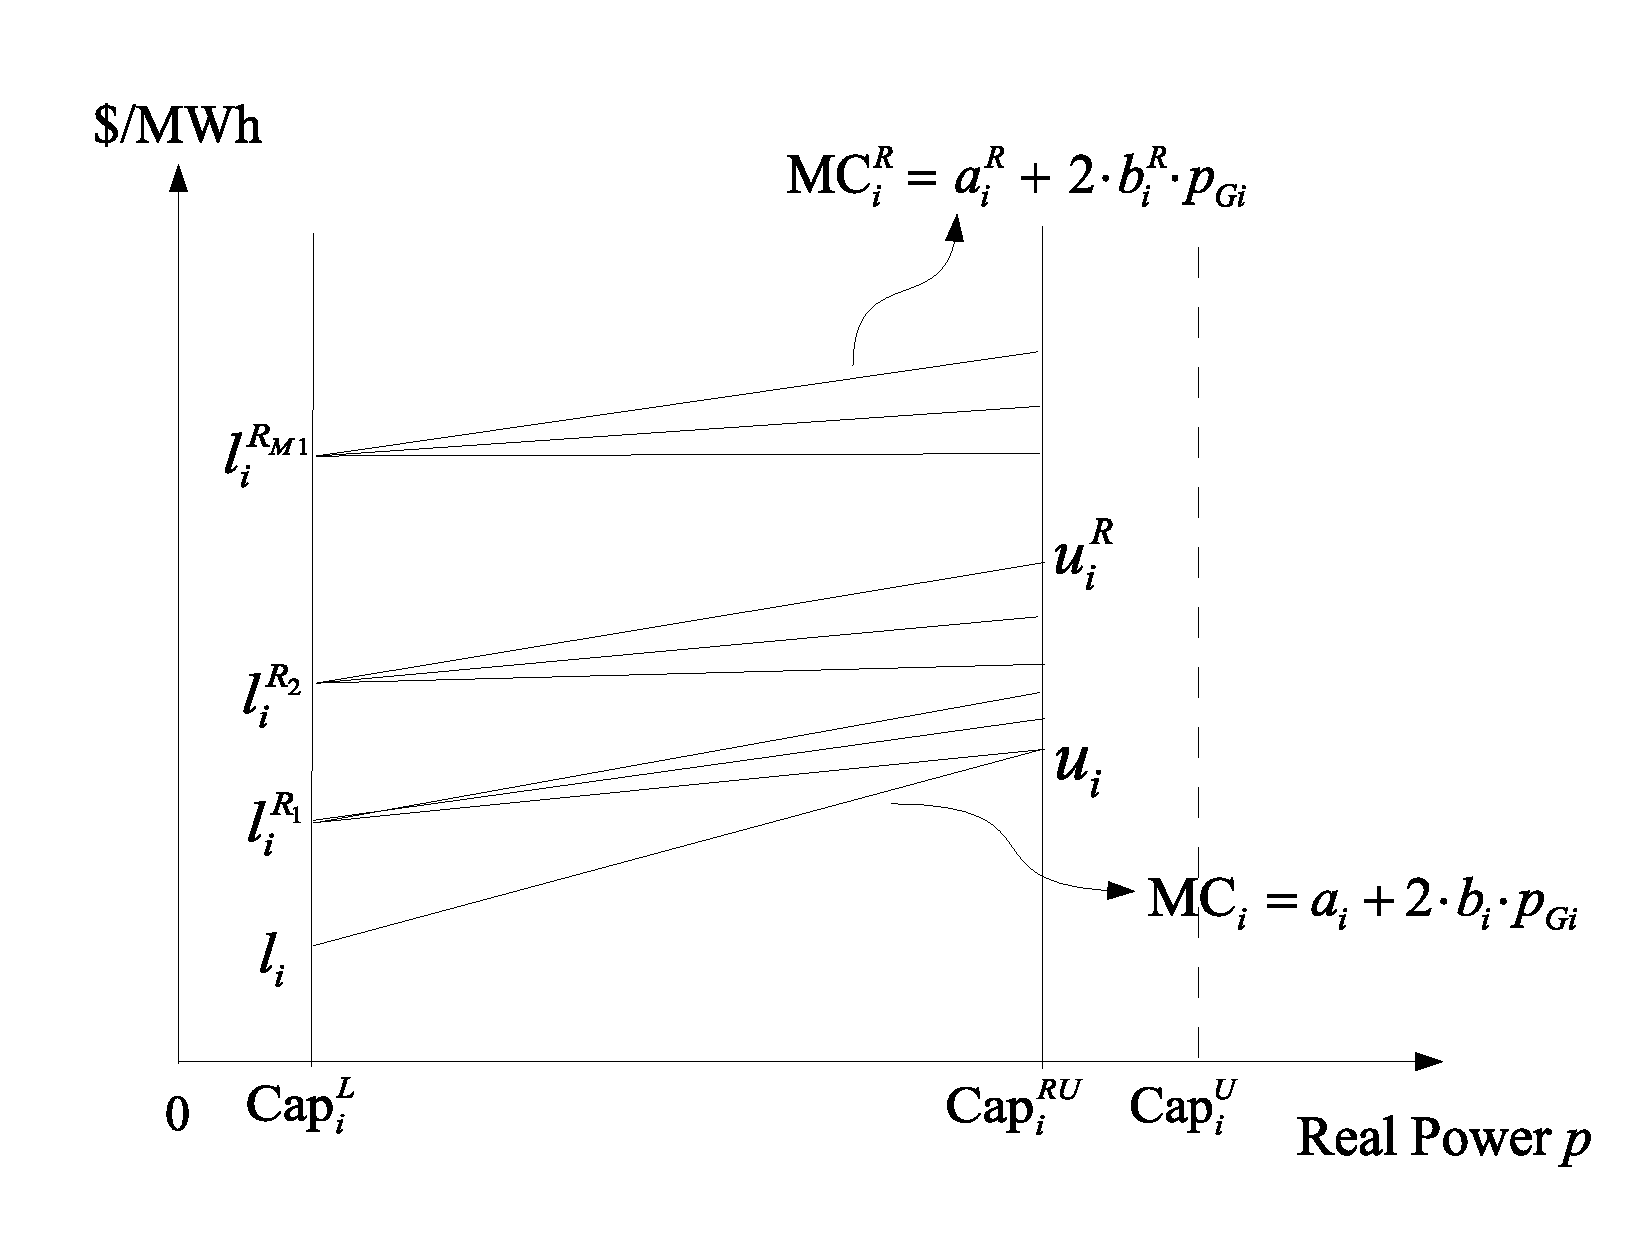
\includegraphics[totalheight = 10cm]{AMES.SupplyOffer.eps}
	\caption{Generator $i$'s Feasible Supply Offers and True Marginal Cost Function}
	\label{fig:supplyOffer}
\end{figure}

\begin{figure}[p]
	\centering
		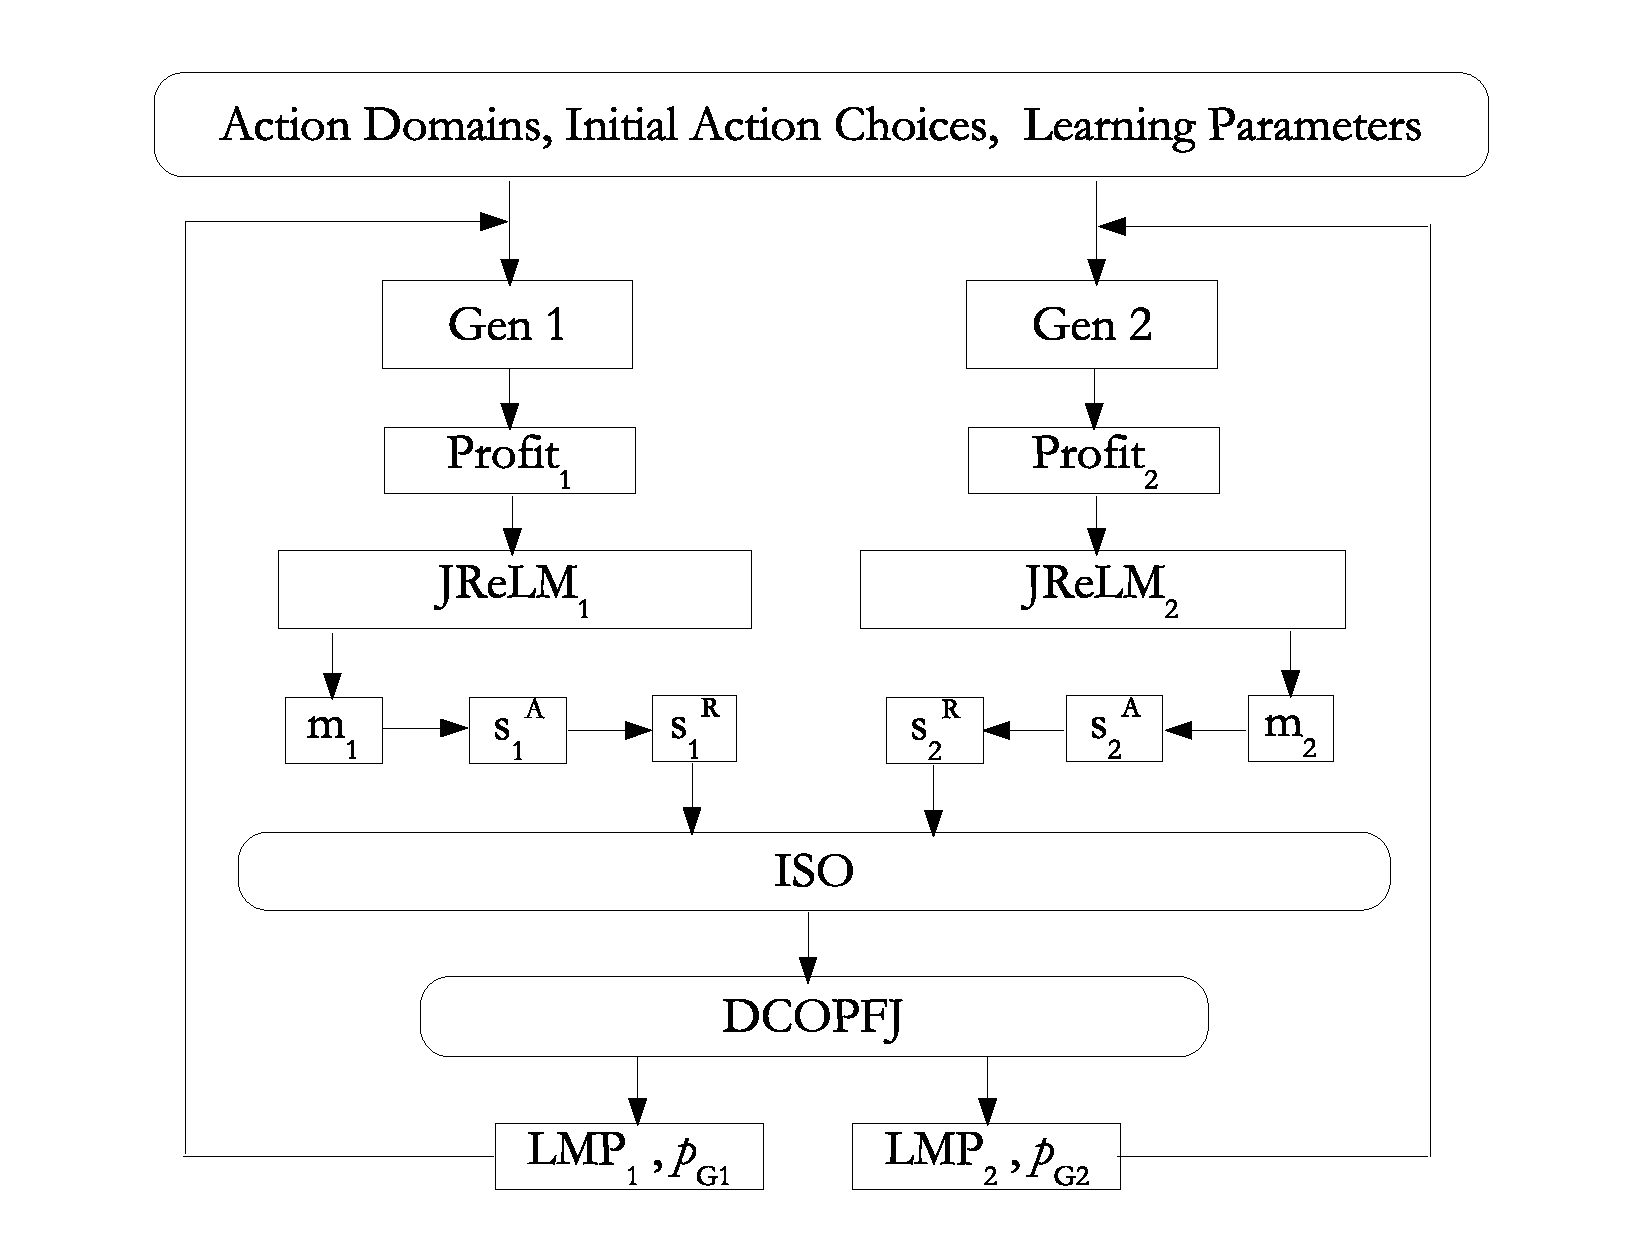
\includegraphics[totalheight = 10cm]{AMES.DynamicFlow.eps}
	\caption{AMES Dynamic Flow with Learning Implementations for Generators 1 and 2}
	\label{fig:dynamicFlow}
\end{figure}

%%%%%%%%%%%%%%%%%%%%%%%%%%%%%%%%%%%%%%%%%


%%%%%%%%TABLES%%%%%%%%%%%%%%%%%%%%%%%%%%%%
%%%%%%%%%%%%%%%%%%%%%%%%%%%%%%%%%%%%%%%%%%


\begin{table}[h]
	\caption{Admissible Exogenous Variables for the AMES Framework} 
	\label{tab:ExogVarAdmissibility}
\begin{minipage}{\textwidth}
	\centering
\begin{tabular}{lll} 

\hline\hline

Variable	& Description & Admissibility Restrictions   \\ [0.5ex]
\hline
 	$K$   & Total number of transmission grid nodes   & $K>0$   \\[0.5ex]
 	$N$   & Total number of distinct network branches & $N>0$   \\[0.5ex]
 	$I$   & Total number of Generators                & $I>0$   \\[0.5ex]
 	$J$   & Total number of LSEs                      & $J>0$   \\[0.5ex]
 	$I_k$ & Set of Generators located at node $k$ &  $\mbox{Card}(\cup_{k=1}^K I_k) = I$ \\[0.5ex]
 	$J_k$ & Set of LSEs located at node $k$       &  $\mbox{Card}(\cup_{k=1}^K J_k) = J$ \\[0.5ex]
  $S_o$       & Base apparent power (three-phase MVAs)            &  $S_o \ge 1$ \\[0.5ex]
  $V_o$       & Base voltage (line-to-line kVs)          &  $V_o > 0$ \\[0.5ex]
  $V_k$       & Voltage magnitude (kVs) at node $k$      &  $V_k = V_o,~k=1,\ldots ,K$ \\[0.5ex]
  $p_{Lj}$    & Real power load (MWs) withdrawn by LSE $j$      & $p_{Lj}\ge 0, ~j=1,\ldots,J$ \\[0.5ex]
  $km$        & Branch connecting nodes $k$ and $m$ (if one exists) &  $k\ne m$ \\[0.5ex]
  $BR$        & Set of all distinct branches $km$, $k < m$ &  $BR\neq \emptyset$\\[0.5ex]
  $X_{km}$    & Reactance (ohms) for branch $km$ & $X_{km}=X_{mk} > 0,~km\in BR$\\[0.5ex]
  $B_{km}$    & $[1/X_{km}]$ for branch $km$                  & $B_{km}=B_{mk} > 0,~km\in BR$\\[0.5ex]
  $P^U_{km}$  & Thermal limit (MWs) for real power flow on $km$  & $P^U_{km} > 0,~km\in BR$\\[0.5ex]
  $\delta_{1} $ & Reference node $1$ voltage angle (radians)  & $ \delta_{1} = 0 $ \\[0.5ex]
  $\pi$     & Soft penalty weight for voltage angle differences  & $\pi > 0$ \\[0.5ex]
  $\mbox{Money}^o_i$  &  Initial money holdings ($\$$) for Gen $i$  &  
              $\mbox{Money}^o_i > 0,~i=1,\ldots,I$\\[0.5ex]
  $\mbox{Cap}^{L}_{i}$  & True lower production limit (MWs) for Gen $i$ 
                & $\mbox{Cap}^L_i \geq 0, ~i=1,\ldots,I$ \\[0.5ex]
  $\mbox{Cap}^{U}_{i}$  & True upper production limit (MWs) for Gen $i$ 
                    & $\mbox{Cap}^{U}_{i} > \mbox{Cap}^L_{i},    ~i=1,\ldots,I$ \\[0.5ex]
  $a_i,b_i$   & True cost coefficients ($\$$/MWh, $\$$/MW$^2$h) for Gen $i$ & $b_i > 0, ~i=1,\ldots,I$ \\[0.5ex]
  $\mbox{MC}_i(p)$  & $\mbox{MC}_i(p) = a_i + 2b_ip$ = Gen $i$'s true MC function   
             &  $\mbox{MC}_i(\mbox{Cap}^L_i) > 0, ~i=1,\ldots,I$ \\[0.5ex]
  $\mbox{FCost}_i$		& Fixed costs (hourly prorated) for Gen $i$ & $\mbox{FCost}_i \ge 0, ~i=1,\ldots,I$ \\[0.5ex] 
  $M_i$	     & Cardinality of the action domain $AD_i$ for Gen $i$  & $M_i  \ge 1,~i=1,\ldots,I$ \\[0.5ex]
  $Mj_{i}$ & Integer-valued density-control parameter for $AD_i$ &  $\prod_{j=1}^3 Mj_{i} = M_i, ~i=1,\ldots,I$\\[0.5ex]
   $\mbox{RIMax}^L_i$ & Range-index parameter for $AD_i$ construction   
           & $\mbox{RIMax}^L_i \in [0,1),~i=1,\ldots,I$\\[0.5ex]
  $\mbox{RIMax}^U_i$ & Range-index parameter for $AD_i$ construction   
           & $\mbox{RIMax}^U_i \in [0,1),~i=1,\ldots,I$\\[0.5ex]
  $\mbox{RIMin}^C_i$ & Range-index parameter for $AD_i$ construction
           & $\mbox{RIMin}^C_i \in (0,1],~i=1,\ldots,I$\\[0.5ex]
  $SS_i$  & Slope-start control parameter for $AD_i$ construction   &  
                $SS_i > 0,~i=1,\ldots,I$ \\[0.5ex]
  $q_i(0)$ & Initial propensity (learning) & Any real value,~$i=1,\ldots,I$\\[0.5ex]
  $C_i$    & Cooling parameter (learning) & $C_i > 0, ~i=1,\ldots,I$\\[0.5ex]
  $r_i$    & Recency parameter (learning) & $0 \le r_i \le 1, ~i=1,\ldots,I$\\[0.5ex]
  $e_i$    & Experimentation parameter (learning) & $0 \le e_i < 1, ~i=1,\ldots,I$\\[0.5ex]
	
\hline
\end{tabular}
\end{minipage}
\end{table}


 \begin{table}[h]
	\caption{Endogenous Variables for the AMES Framework} 
	\label{tab:EndogVariables}
\begin{minipage}{\textwidth}
	\centering
\begin{tabular}{ll} % centered columns (2 columns)

\hline\hline

Variable	& Description    \\ [0.5ex]
\hline
$p_{Gi}$    &  Real power injection (MWs) by Gen $i=1,\ldots, I$   \\[0.5ex]
$\delta_k$  &  Voltage angle (radians) at node $k = 2,\ldots , K$           \\[0.5ex]
$\mbox{LMP}_k$  & Locational marginal price ($\$$/MWh) at node $k=1,\ldots, K$ \\[0.5ex]
$P_{km}$   & Real power (MWs) flowing in branch $km ~\in ~ \mbox{BR}$ \\[0.5ex]
$\mbox{PGen}_k$ & Total real power injection (MWs) at node $k=1,\ldots ,K$ \\[0.5ex]
$\mbox{PLoad}_k$ & Total real power withdrawal (MWs) at node $k=1,\ldots,K$ \\[0.5ex]
$\mbox{PNetInject}_k$ &  Total net real power injection (MWs) at node $k =1,\ldots,K$ \\[0.5ex]
$\mbox{Profit}_i$  & Realized profit ($\$$/h) for Gen $i=1,\ldots, I$   \\[0.5ex]
$\mbox{Money}_i$  & Cumulative money holdings ($\$$) for Gen $i=1,\ldots, I$   \\[0.5ex]
$\mbox{Cap}^{RL}_{i}$    & Reported lower production limit (MWs) for Gen $i=1,\ldots,I$ \\[0.5ex]
$\mbox{Cap}^{RU}_{i}$  & Reported upper production limit (MWs) for Gen $i=1,\ldots,I$ \\[0.5ex]
$a_i^R,b_i^R$ & Reported cost coefficients ($\$$/MWh, $\$$/MW$^2$h) for Gen $i=1,\ldots, I$ \\[0.5ex]

\hline
\end{tabular}
\end{minipage}
\end{table}




\begin{table}[h]
	\caption{Dynamic 5-Node Test Case -- DC-OPF Structural Input Data (SI)} 
	\label{tab: 5NodeInput}
\begin{minipage}{\textwidth}
	\centering
\begin{tabular}{cccccccccc} 

\hline\hline\\[0.1ex]
Base Values 
  	& \mbox{}	\\
$S_o$ &	$V_o$	\\	
   100.0	     &     10.0		\\ \\

$K$%
\footnote{Total number of nodes}
 & $\pi$%
\footnote{Soft penalty weight $\pi$ for voltage angle differences}
  \\
5 &  0.05   \\
  
\\ Branch \\ 
From&	To&	lineCap%
\footnote{Upper limit $P^U_{km}$ (in MWs) on the magnitude of real power flow in branch $km$} &  $X$%
\footnote{Reactance $X_{km}$ (in ohms) for branch $km$}
 \\[0.5ex]
 	1 & 2 & 250.0	& 0.0281     \\
 	1 & 4 & 150.0	& 0.0304     \\
 	1 & 5 & 400.0	& 0.0064     \\
	2 & 3 & 350.0	& 0.0108     \\
	3 & 4 & 240.0	& 0.0297     \\
	4 & 5 & 240.0	& 0.0297     \\

  
\\ 
Gen ID & atNode & FCost   &  $a$     &   $b$    & Cap$^L$    & Cap$^U$     &  Init$\$$ \\[0.5ex]
  1	& 1	& 1600.0  & 14.0   & 0.005     & 0.0	   & 110.0       &  $\$1.0M$    \\
  2	& 1	& 1200.0  & 15.0   & 0.006     & 0.0	   & 100.0       &  $\$1.0M$  \\
  3	& 3	& 8500.0  & 25.0   & 0.010     & 0.0	   & 520.0       &  $\$1.0M$ \\
  4	& 4	& 1000.0  & 30.0   & 0.012     & 0.0	   & 200.0       &  $\$1.0M$ \\
  5	& 5	& 5400.0  & 10.0   & 0.007     & 0.0	   & 600.0       &  $\$1.0M$ \\



\\ LSE \\ ID &	atNode & L-00%
\footnote{L-H: Load L (in MWs) for hour H, where H=00,01,...,23}
 & L-01	& L-02	& L-03	& L-04	& L-05	& L-06	& L-07\\[0.5ex]
1	&	2	&	350.00	&	322.93	&	305.04	&	296.02	&	287.16	&	291.59	&	296.02	&	314.07 \\
2	&	3	&	300.00	&	276.80	&	261.47	&	253.73	&	246.13	&	249.93	&	253.73	&	269.20 \\
3	&	4	&	250.00	&	230.66	&	217.89	&	211.44	&	205.11	&	208.28	&	211.44	&	224.33 \\

ID &	atNode & L-08 & L-09	& L-10	& L-11	& L-12	& L-13	& L-14	& L-15\\[0.5ex]
1	&	2	&	358.86	&	394.80	&	403.82	&	408.25	&	403.82	&	394.80	&	390.37	&	390.37 \\
2	&	3	&	307.60	&	338.40	&	346.13	&	349.93	&	346.13	&	338.40	&	334.60	&	334.60 \\
3	&	4	&	256.33	&	282.00	&	288.44	&	291.61	&	288.44	&	282.00	&	278.83	&	278.83 \\

ID &	atNode & L-16 & L-17	& L-18	& L-19	& L-20	& L-21	& L-22	& L-23\\[0.5ex]
1	&	2	&	408.25	&	448.62	&	430.73	&	426.14	&	421.71	&	412.69	&	390.37	&	363.46 \\ 
2	&	3	&	349.93	&	384.53	&	369.20	&	365.26	&	361.47	&	353.73	&	334.60	&	311.53 \\ 
3	&	4	&	291.61	&	320.44	&	307.67	&	304.39	&	301.22	&	294.78	&	278.83	&	259.61 \\

\hline
\end{tabular}
\end{minipage}
\end{table}


\begin{table}[h]
	\caption{Dynamic 5-Node Test Case -- Action Domain and Learning Input Data} 
	\label{tab: 5NodeInput.Learning}
\begin{minipage}{\textwidth}
	\centering
\begin{tabular}{cccccccccccc} 

\hline\hline\\[0.1ex]

\multicolumn{8}{c}{Action Domain Parameters} \\ [0.5ex]

\\Gen ID   &  $M1$  & $M2$   &  $M3$  &  RIMax$^L$ & RIMax$^U$  & ~RIMin$^C$ &  $SS$    \\[0.5ex]
     1	   &  10    & 10     &  1     &  0.75      & 0.75	 &  1.00      &  0.001   \\
     2	   &  10    & 10     &  1     &  0.75      & 0.75	 &  1.00      &  0.001   \\
     3	   &  10    & 10     &  1     &  0.75      & 0.75	 &  1.00      &  0.001   \\
     4	   &  10    & 10     &  1     &  0.75      & 0.75	 &  1.00      &  0.001   \\
     5	   &  10    & 10     &  1     &  0.75      & 0.75	 &  1.00      &  0.001   \\ 

\\

\multicolumn{8}{c}{Learning Parameters} \\ [0.5ex]

\\Gen ID   & $q(0)$  & $C$  & $r$  &  $e$    \\[0.5ex]
     1	   &  6000.0  & 1000.0 & 0.04 & 0.97 \\
     2	   &  6000.0  & 1000.0 & 0.04 & 0.97 \\
     3	   &  6000.0  & 1000.0 & 0.04 & 0.97 \\
     4	   &  6000.0  & 1000.0 & 0.04 & 0.97 \\
     5	   &  6000.0  & 1000.0 & 0.04 & 0.97 \\

\\ \multicolumn{8}{c}{Initial Seed Values for All 20 Runs} \\ [0.5ex]

\\\multicolumn{4}{c}{~~RunID~~InitialSeed} & \multicolumn{4}{c}{RunID~~InitialSeed}   \\[0.5ex]

\multicolumn{4}{c}{~~~~01~~~~~695672061} &  \multicolumn{4}{c}{~~11~~~~-597305450} \\
\multicolumn{4}{c}{~~~~02~~~~~857398845} &  \multicolumn{4}{c}{~~12~~~~-494232424} \\
\multicolumn{4}{c}{~~~~03~~~~~507304343} &  \multicolumn{4}{c}{~~13~~~~-158932839} \\
\multicolumn{4}{c}{~~~~04~~~~~748974391} &	\multicolumn{4}{c}{~~14~~~~-934341230} \\
\multicolumn{4}{c}{~~~~05~~~~~494375928} &	\multicolumn{4}{c}{~~15~~~~-734837588} \\
\multicolumn{4}{c}{~~~~06~~~~~289658396} &	\multicolumn{4}{c}{~~16~~~~-219860821} \\
\multicolumn{4}{c}{~~~~07~~~~~158324732} &	\multicolumn{4}{c}{~~17~~~~-845925752} \\
\multicolumn{4}{c}{~~~~08~~~~~324702357} &	\multicolumn{4}{c}{~~18~~~~-367413463} \\
\multicolumn{4}{c}{~~~~09~~~~~903534301} &	\multicolumn{4}{c}{~~19~~~~-629523701} \\
\multicolumn{4}{c}{~~~~10~~~~~205753353} &	\multicolumn{4}{c}{~~20~~~~-257802760} \\

\hline
\end{tabular}
\end{minipage}
\end{table}




\begin{table}[h]
	\caption{No-Learning Dynamic 5-Node Test Case -- Solution Value (SI) for Real Power Branch Flow $P_{km}$, with Associated Thermal Limit $P_{km}^U$, for Each Distinct Branch $km$} 
	\label{tab: 5Node.NoLearning.BranchFlows}
\begin{minipage}{\textwidth}
	\centering
\begin{tabular}{crrrrrr} 
\hline\hline
\\[0.1ex]

Hour & $P_{12}$\footnote{In accordance with the usual convention, the real power $P_{km}$ flowing along a branch $km$ is positively valued if and only if real power is flowing from node $k$ to node $m$.}  & $P_{14}~~$ & $P_{15}~~$ & $P_{23}~~$ & $P_{34}~~$ & $P_{45}~~$ \\
\hline
00	&	250.00	&	129.65	&	-255.77	&	-100.00	&	-67.47	&	-187.82	\\
01  & 250.00	&	126.71	&	-253.27	&	-72.93	&	-80.32	&	-184.27	\\
02	&	250.00	&	124.77	&	-251.61	&	-55.04	&	-88.81	&	-181.93	\\
03	&	250.00	&	123.79	&	-250.77	&	-46.02	&	-93.09	&	-180.74	\\
04	&	250.00	&	122.83	&	-249.95	&	-37.16	&	-97.30	&	-179.58	\\
05	&	250.00	&	123.31	&	-250.36	&	-41.59	&	-95.19	&	-180.16	\\
06	&	250.00	&	123.79	&	-250.77	&	-46.02	&	-93.09	&	-180.74	\\
07	&	250.00	&	125.75	&	-252.45	&	-64.07	&	-84.52	&	-183.11	\\
08	&	250.00	&	130.61	&	-256.60	&	-108.86	&	-63.26	&	-188.98	\\
09	&	250.00	&	134.51	&	-259.92	&	-144.80	&	-46.20	&	-193.69	\\
10	&	250.00	&	135.49	&	-260.76	&	-153.82	&	-41.92	&	-194.87	\\
11	&	250.00	&	135.97	&	-261.17	&	-158.25	&	-39.81	&	-195.45	\\
12	&	250.00	&	135.49	&	-260.76	&	-153.82	&	-41.92	&	-194.87	\\
13	&	250.00	&	134.51	&	-259.92	&	-144.80	&	-46.20	&	-193.69	\\
14	&	250.00	&	134.03	&	-259.51	&	-140.37	&	-48.30	&	-193.11	\\
15	&	250.00	&	134.03	&	-259.51	&	-140.37	&	-48.30	&	-193.11	\\
16	&	250.00	&	135.97	&	-261.17	&	-158.25	&	-39.81	&	-195.45	\\
17	&	250.00	&	 98.83	&	-346.76	&	-198.62	&	-63.15	&	-175.88	\\
18	&	250.00	&	137.64	&	-274.17	&	-180.73	&	-29.93	&	-199.96	\\
19	&	250.00	&	137.91	&	-262.83	&	-176.14	&	-31.32	&	-197.80	\\
20	&	250.00	&	137.43	&	-262.42	&	-171.71	&	-33.42	&	-197.22	\\
21	&	250.00	&	136.45	&	-261.58	&	-162.69	&	-37.71	&	-196.03	\\
22	&	250.00	&	134.03	&	-259.51	&	-140.37	&	-48.30	&	-193.11	\\
23	&	250.00	&	131.11	&	-257.02	&	-113.46	&	-61.08	&	-189.58	\\

\hline \\[0.05ex]
& $P_{12}^U~~$ & $P_{14}^U~~$ & $P_{15}^U~~$ & $P_{23}^U~~$ & $P_{34}^U~~$ & $P_{45}^U~~$ \\
&	250.00	&	150.00	&	400.00	&	350.00	&	240.00	&	240.00	\\
\hline
\end{tabular}
\end{minipage}
\end{table}


\begin{table}[h]
	\caption{No-Learning Dynamic 5-Node Test Case -- Solution Values (SI) for Real Power Production Levels 
and Associated Upper Production Limits, together with LMPs (Nodal Balance Constraint Multipliers) and Minimum Total Variable Cost} 
	\label{tab: 5Node.NoLearning.ProdsLMPsMinTVC}
\begin{minipage}{\textwidth}
	\centering
\begin{tabular}{crrrrrrrrrrr} 
\hline\hline \\[0.1ex]
Hour & $p_{G1}^\ast~$ & $p_{G2}^\ast$ & $p_{G3}^\ast~$ &  $p_{G4}^\ast$ & $p_{G5}^\ast~$ 
& $\mbox{LMP}_1$ & $\mbox{LMP}_2$ & $\mbox{LMP}_3$ & $\mbox{LMP}_4$ & $\mbox{LMP}_5$  & minTVC \\
\hline
0	&	110.0	&	13.9	&	332.5	&	0.0	&	443.6	&	15.17	&	35.50	&	31.65	&	21.05	&	16.21	&	19587.1	\\
1	&	110.0	&	13.4	&	269.4	&	0.0	&	437.5	&	15.16	&	33.95	&	30.39	&	20.60	&	16.13	&	17107.3	\\
2	&	110.0	&	13.2	&	227.7	&	0.0	&	433.5	&	15.16	&	32.92	&	29.55	&	20.30	&	16.07	&	15556.8	\\
3	&	110.0	&	13.0	&	206.7	&	0.0	&	431.5	&	15.16	&	32.40	&	29.13	&	20.15	&	16.04	&	14800.9	\\
4	&	110.0	&	12.9	&	186.0	&	0.0	&	429.5	&	15.15	&	31.89	&	28.72	&	20.00	&	16.01	&	14076.1	\\
5	&	110.0	&	13.0	&	196.3	&	0.0	&	430.5	&	15.16	&	32.15	&	28.93	&	20.07	&	16.03	&	14436.5	\\
6	&	110.0	&	13.0	&	206.7	&	0.0	&	431.5	&	15.16	&	32.40	&	29.13	&	20.15	&	16.04	&	14800.9	\\
7	&	110.0	&	13.3	&	248.8	&	0.0	&	435.6	&	15.16	&	33.44	&	29.97	&	20.45	&	16.10	&	16330.2	\\
8	&	110.0	&	14.0	&	353.2	&	0.0	&	445.6	&	15.17	&	36.01	&	32.06	&	21.20	&	16.24	&	20433.9	\\
9	&	110.0	&	14.6	&	437.0	&	0.0	&	453.6	&	15.18	&	38.08	&	33.74	&	21.81	&	16.35	&	24043.6	\\
10	&	110.0	&	14.7	&	458.0	&	0.0	&	455.6	&	15.18	&	38.60	&	34.16	&	21.96	&	16.38	&	24993.9	\\
11	&	110.0	&	14.8	&	468.4	&	0.0	&	456.6	&	15.18	&	38.85	&	34.37	&	22.03	&	16.39	&	25467.5	\\
12	&	110.0	&	14.7	&	458.0	&	0.0	&	455.6	&	15.18	&	38.60	&	34.16	&	21.96	&	16.38	&	24993.9	\\
13	&	110.0	&	14.6	&	437.0	&	0.0	&	453.6	&	15.18	&	38.08	&	33.74	&	21.81	&	16.35	&	24043.6	\\
14	&	110.0	&	14.5	&	426.7	&	0.0	&	452.6	&	15.17	&	37.82	&	33.53	&	21.73	&	16.34	&	23583.1	\\
15	&	110.0	&	14.5	&	426.7	&	0.0	&	452.6	&	15.17	&	37.82	&	33.53	&	21.73	&	16.34	&	23583.1	\\
16	&	110.0	&	14.8	&	468.4	&	0.0	&	456.6	&	15.18	&	38.85	&	34.37	&	22.03	&	16.39	&	25467.5	\\
17	&	2.1	&	0.0	&	520.0	&	108.9	&	522.6	&	14.02	&	78.24	&	66.07	&	32.61	&	17.32	&	31038.5	\\
18	&	107.4	&	6.1	&	520.0	&	0.0	&	474.1	&	15.07	&	45.55	&	39.78	&	23.90	&	16.64	&	28006.9	\\
19	&	110.0	&	15.1	&	510.1	&	0.0	&	460.6	&	15.18	&	39.88	&	35.20	&	22.33	&	16.45	&	27422.4	\\
20	&	110.0	&	15.0	&	499.8	&	0.0	&	459.6	&	15.18	&	39.63	&	35.00	&	22.26	&	16.43	&	26931.9	\\
21	&	110.0	&	14.9	&	478.7	&	0.0	&	457.6	&	15.18	&	39.11	&	34.57	&	22.11	&	16.41	&	25945.9	\\
22	&	110.0	&	14.5	&	426.7	&	0.0	&	452.6	&	15.17	&	37.82	&	33.53	&	21.73	&	16.34	&	23583.1	\\
23	&	110.0	&	14.1	&	363.9	&	0.0	&	446.6	&	15.17	&	36.28	&	32.28	&	21.28	&	16.25	&	20879.5	\\

\hline \\[0.05ex]
& $\mbox{Cap}_1^U$ & $\mbox{Cap}_2^U$ & $\mbox{Cap}_3^U$ & $\mbox{Cap}_4^U$ & $\mbox{Cap}_5^U$  \\
&	110.0	&	100.0	&	520.0	&	200.0	&	600.0	\\
\hline
\end{tabular}
\end{minipage}
\end{table}



\begin{table}[h]
	\caption{Learning Dynamic 5-Node Test Case -- Mean and Standard Deviation for Solution Value (SI) on Day 422 for Real Power Branch Flow $P_{km}$, with Associated Thermal Limit $P_{km}^U$, for Each Distinct Branch $km$} 
	\label{tab: 5Node.Learning.BranchFlows}
\begin{minipage}{\textwidth}
	\centering
\begin{tabular}{crrrrrrrrrrrr} 
\hline\hline \\[0.1ex]
Hour & $\overline{P_{12}}~$ & $P_{12}^{SD}$ & $\overline{P_{14}}$ & $P_{14}^{SD}$ & $\overline{P_{15}}~$ & $P_{15}^{SD}$ &  $\overline{P_{23}}~$ & $P_{23}^{SD}$ & $\overline{P_{34}}~$ & $P_{34}^{SD}$ & $\overline{P_{45}}~$ & $P_{45}^{SD}~$\\
\hline
00	&	249.3	&	3.3	&	77.0	&	9.2	&	-116.5	&	10.4	&	-100.7	&	3.3	&	-120.3	&	9.6	&	-103.9	&	11.6	\\
01	&	248.0	&	6.4	&	74.8	&	11.7	&	-113.2	&	13.9	&	-74.9	&	6.4	&	-130.8	&	13.1	&	-100.9	&	14.7	\\
02	&	247.1	&	9.1	&	73.7	&	13.3	&	-111.3	&	16.7	&	-58.0	&	9.1	&	-137.3	&	16.2	&	-99.4	&	16.9	\\
03	&	246.4	&	10.5	&	73.2	&	14.2	&	-110.3	&	18.3	&	-49.6	&	10.5	&	-140.1	&	17.8	&	-98.7	&	18.1	\\
04	&	245.5	&	12.0	&	72.6	&	15.2	&	-108.9	&	20.1	&	-41.6	&	12.0	&	-142.8	&	19.5	&	-97.8	&	19.4	\\
05	&	246.0	&	11.2	&	72.9	&	14.7	&	-109.6	&	19.2	&	-45.6	&	11.2	&	-141.5	&	18.6	&	-98.2	&	18.7	\\
06	&	246.4	&	10.5	&	73.2	&	14.2	&	-110.3	&	18.3	&	-49.6	&	10.5	&	-140.1	&	17.8	&	-98.7	&	18.1	\\
07	&	247.5	&	7.8	&	74.1	&	12.5	&	-112.1	&	15.3	&	-66.5	&	7.8	&	-134.1	&	14.7	&	-100.0	&	15.8	\\
08	&	249.4	&	2.9	&	77.8	&	8.5	&	-117.3	&	9.5	&	-109.5	&	2.9	&	-116.5	&	8.7	&	-104.8	&	10.6	\\
09	&	249.8	&	1.1	&	80.7	&	5.6	&	-120.6	&	5.9	&	-145.0	&	1.1	&	-101.0	&	5.7	&	-108.6	&	7.0	\\
10	&	249.9	&	0.6	&	81.4	&	5.1	&	-121.4	&	5.2	&	-154.0	&	0.6	&	-97.1	&	5.1	&	-109.5	&	6.3	\\
11	&	249.9	&	0.4	&	81.8	&	4.8	&	-121.9	&	4.9	&	-158.3	&	0.4	&	-95.1	&	4.9	&	-110.0	&	6.0	\\
12	&	249.9	&	0.6	&	81.4	&	5.1	&	-121.4	&	5.2	&	-154.0	&	0.6	&	-97.1	&	5.1	&	-109.5	&	6.3	\\
13	&	249.8	&	1.1	&	80.7	&	5.6	&	-120.6	&	5.9	&	-145.0	&	1.1	&	-101.0	&	5.7	&	-108.6	&	7.0	\\
14	&	249.7	&	1.3	&	80.3	&	5.9	&	-120.2	&	6.3	&	-140.7	&	1.3	&	-102.9	&	6.1	&	-108.1	&	7.4	\\
15	&	249.7	&	1.3	&	80.3	&	5.9	&	-120.2	&	6.3	&	-140.7	&	1.3	&	-102.9	&	6.1	&	-108.1	&	7.4	\\
16	&	249.9	&	0.4	&	81.8	&	4.8	&	-121.9	&	4.9	&	-158.3	&	0.4	&	-95.1	&	4.9	&	-110.0	&	6.0	\\
17	&	250.0	&	0.0	&	85.3	&	3.2	&	-125.5	&	3.2	&	-198.6	&	0.0	&	-77.0	&	3.3	&	-114.4	&	3.9	\\
18	&	250.0	&	0.0	&	83.6	&	4.1	&	-123.8	&	4.1	&	-180.7	&	0.0	&	-85.2	&	4.2	&	-112.3	&	5.1	\\
19	&	250.0	&	0.0	&	83.2	&	4.2	&	-123.4	&	4.2	&	-176.1	&	0.0	&	-87.3	&	4.3	&	-111.7	&	5.1	\\
20	&	250.0	&	0.0	&	82.9	&	4.3	&	-123.0	&	4.3	&	-171.7	&	0.0	&	-89.3	&	4.4	&	-111.3	&	5.3	\\
21	&	250.0	&	0.2	&	82.1	&	4.6	&	-122.3	&	4.6	&	-162.7	&	0.2	&	-93.2	&	4.7	&	-110.4	&	5.7	\\
22	&	249.7	&	1.3	&	80.3	&	5.9	&	-120.2	&	6.3	&	-140.7	&	1.3	&	-102.9	&	6.1	&	-108.1	&	7.4	\\
23	&	249.4	&	2.7	&	78.1	&	8.1	&	-117.7	&	9.0	&	-114.0	&	2.7	&	-114.5	&	8.3	&	-105.3	&	10.1	\\

\hline \\[0.05ex]
& $P_{12}^U~$ & & $P_{14}^U~$ & & $P_{15}^U~$ & & $P_{23}^U~$ & & $P_{34}^U~$ & & $P_{45}^U~$ \\
&	250.0	& &	150.0	& &	400.0	& &	350.0	& &	240.0	& &	240.0	\\

\hline
\end{tabular}
\end{minipage}
\end{table}

\begin{table}[h]
	\caption{Learning Dynamic 5-Node Test Case -- Means and Standard Deviations for Solution Values (SI) on Day 422 for Real Power Production Levels} 
	\label{tab: 5Node.Learning.Prods}
\begin{minipage}{\textwidth}
	\centering
\begin{tabular}{crrrrrrrrrr} 
\hline\hline \\[0.1ex]
Hour & $\overline{p_{G1}^\ast}~$ & $p_{G1}^{\ast SD}$ & $\overline{p_{G2}^\ast}~$ & $p_{G2}^{\ast SD}$ & $\overline{p_{G3}^\ast}~$ & $p_{G3}^{\ast SD}$ & $\overline{p_{G4}^\ast}~$ & $p_{G4}^{\ast SD}$ & $\overline{p_{G5}^\ast}~$ & $p_{G5}^{\ast SD}$\\
\hline
00	&	110.00	&	0.00	&	99.80	&	0.88	&	280.40	&	10.92	&	189.37	&	29.60	&	220.42	&	21.84	\\
01	&	109.92	&	0.36	&	99.64	&	1.59	&	220.92	&	17.07	&	185.74	&	37.25	&	214.17	&	28.21	\\
02	&	109.85	&	0.67	&	99.53	&	2.10	&	182.18	&	22.66	&	182.11	&	42.50	&	210.73	&	32.93	\\
03	&	109.81	&	0.83	&	99.47	&	2.35	&	163.20	&	25.51	&	179.72	&	45.31	&	208.98	&	35.57	\\
04	&	109.78	&	0.98	&	99.42	&	2.60	&	144.96	&	28.69	&	177.50	&	48.31	&	206.74	&	38.51	\\
05	&	109.80	&	0.91	&	99.45	&	2.48	&	154.08	&	27.03	&	178.61	&	46.79	&	207.86	&	37.00	\\
06	&	109.81	&	0.83	&	99.47	&	2.35	&	163.20	&	25.51	&	179.72	&	45.31	&	208.98	&	35.57	\\
07	&	109.88	&	0.52	&	99.59	&	1.84	&	201.60	&	19.83	&	184.36	&	39.92	&	212.17	&	30.52	\\
08	&	110.00	&	0.00	&	99.81	&	0.86	&	300.60	&	9.85	&	190.23	&	27.16	&	222.16	&	19.91	\\
09	&	110.00	&	0.00	&	99.82	&	0.80	&	382.48	&	5.95	&	193.70	&	18.22	&	229.20	&	12.83	\\
10	&	110.00	&	0.00	&	99.82	&	0.79	&	403.03	&	5.22	&	194.57	&	16.43	&	230.97	&	11.41	\\
11	&	110.00	&	0.00	&	99.83	&	0.78	&	413.12	&	4.92	&	195.00	&	15.65	&	231.84	&	10.81	\\
12	&	110.00	&	0.00	&	99.82	&	0.79	&	403.03	&	5.22	&	194.57	&	16.43	&	230.97	&	11.41	\\
13	&	110.00	&	0.00	&	99.82	&	0.80	&	382.48	&	5.95	&	193.70	&	18.22	&	229.20	&	12.83	\\
14	&	110.00	&	0.00	&	99.82	&	0.81	&	372.38	&	6.36	&	193.27	&	19.19	&	228.33	&	13.60	\\
15	&	110.00	&	0.00	&	99.82	&	0.81	&	372.38	&	6.36	&	193.27	&	19.19	&	228.33	&	13.60	\\
16	&	110.00	&	0.00	&	99.83	&	0.78	&	413.12	&	4.92	&	195.00	&	15.65	&	231.84	&	10.81	\\
17	&	110.00	&	0.00	&	99.84	&	0.71	&	506.19	&	3.25	&	197.68	&	10.36	&	239.88	&	7.11	\\
18	&	110.00	&	0.00	&	99.83	&	0.74	&	464.70	&	4.18	&	197.02	&	13.32	&	236.04	&	9.13	\\
19	&	110.00	&	0.00	&	99.83	&	0.75	&	454.09	&	4.26	&	196.73	&	13.57	&	235.14	&	9.30	\\
20	&	110.00	&	0.00	&	99.83	&	0.76	&	443.90	&	4.37	&	196.30	&	13.91	&	234.36	&	9.53	\\
21	&	110.00	&	0.00	&	99.83	&	0.77	&	423.24	&	4.69	&	195.43	&	14.97	&	232.71	&	10.29	\\
22	&	110.00	&	0.00	&	99.82	&	0.81	&	372.38	&	6.36	&	193.27	&	19.19	&	228.33	&	13.60	\\
23	&	110.00	&	0.00	&	99.81	&	0.86	&	311.06	&	9.30	&	190.67	&	25.92	&	223.06	&	18.93	\\

\hline \\[0.05ex]
& $\mbox{Cap}_1^U$ & & $\mbox{Cap}_2^U$ & & $\mbox{Cap}_3^U$ & & $\mbox{Cap}_4^U$ & & $\mbox{Cap}_5^U$ & \\
&	110.0	& &	100.0	& &	520.0	& &	200.0	& &	600.0	\\

\hline
\end{tabular}
\end{minipage}
\end{table}


\begin{table}[h]
	\caption{Learning Dynamic 5-Node Test Case - Means and Standard Deviations for Solution Values (SI) on Day 422 for LMPs (Nodal Balance Constraint Multipliers) } 
	\label{tab: 5Node.Learning.LMPs}
\begin{minipage}{\textwidth}
	\centering
\begin{tabular}{crcrcrcrcrc} 
\hline\hline \\[0.1ex]
Hour & $\overline{\mbox{LMP}_1}$ & $\mbox{LMP}_1^{SD}$ & $\overline{\mbox{LMP}_2}$ & $\mbox{LMP}_2^{SD}$ & $\overline{\mbox{LMP}_3}$ & $\mbox{LMP}_3^{SD}$ & $\overline{\mbox{LMP}_4}$ & $\mbox{LMP}_4^{SD}$ & $\overline{\mbox{LMP}_5}$ & $\mbox{LMP}_5^{SD}$\\
\hline
00	&	52.74	&	12.33	&	110.30	&	58.16	&	99.39	&	48.02	&	69.40	&	21.56	&	55.70	&	13.06	\\
01	&	52.70	&	12.26	&	100.56	&	49.61	&	91.49	&	41.16	&	66.56	&	19.44	&	55.16	&	12.82	\\
02	&	52.68	&	12.23	&	94.18	&	44.34	&	86.32	&	36.92	&	64.69	&	18.12	&	54.81	&	12.67	\\
03	&	52.66	&	12.22	&	91.02	&	41.79	&	83.75	&	34.86	&	63.77	&	17.46	&	54.63	&	12.60	\\
04	&	52.63	&	12.23	&	87.96	&	39.38	&	81.27	&	32.90	&	62.86	&	16.84	&	54.45	&	12.54	\\
05	&	52.65	&	12.23	&	89.49	&	40.57	&	82.51	&	33.86	&	63.32	&	17.15	&	54.54	&	12.57	\\
06	&	52.66	&	12.22	&	91.02	&	41.79	&	83.75	&	34.86	&	63.77	&	17.46	&	54.63	&	12.60	\\
07	&	52.69	&	12.24	&	97.38	&	46.96	&	88.91	&	39.03	&	65.63	&	18.78	&	54.98	&	12.75	\\
08	&	52.75	&	12.37	&	113.52	&	61.04	&	102.01	&	50.33	&	70.35	&	22.28	&	55.87	&	13.15	\\
09	&	52.79	&	12.56	&	126.59	&	73.16	&	112.61	&	60.05	&	74.15	&	25.31	&	56.58	&	13.52	\\
10	&	52.80	&	12.62	&	129.87	&	76.28	&	115.27	&	62.55	&	75.11	&	26.09	&	56.75	&	13.61	\\
11	&	52.80	&	12.65	&	131.48	&	77.83	&	116.57	&	63.79	&	75.58	&	26.48	&	56.84	&	13.66	\\
12	&	52.80	&	12.62	&	129.87	&	76.28	&	115.27	&	62.55	&	75.11	&	26.09	&	56.75	&	13.61	\\
13	&	52.79	&	12.56	&	126.59	&	73.16	&	112.61	&	60.05	&	74.15	&	25.31	&	56.58	&	13.52	\\
14	&	52.78	&	12.53	&	124.98	&	71.64	&	111.30	&	58.83	&	73.68	&	24.93	&	56.49	&	13.47	\\
15	&	52.78	&	12.53	&	124.98	&	71.64	&	111.30	&	58.83	&	73.68	&	24.93	&	56.49	&	13.47	\\
16	&	52.80	&	12.65	&	131.48	&	77.83	&	116.57	&	63.79	&	75.58	&	26.48	&	56.84	&	13.66	\\
17	&	52.73	&	12.81	&	147.26	&	92.89	&	129.34	&	75.90	&	80.10	&	30.38	&	57.58	&	14.07	\\
18	&	52.80	&	12.81	&	139.68	&	85.72	&	123.22	&	70.13	&	77.95	&	28.50	&	57.26	&	13.93	\\
19	&	52.80	&	12.78	&	138.00	&	84.10	&	121.86	&	68.83	&	77.46	&	28.08	&	57.17	&	13.87	\\
20	&	52.80	&	12.75	&	136.38	&	82.54	&	120.55	&	67.58	&	77.00	&	27.68	&	57.09	&	13.82	\\
21	&	52.81	&	12.68	&	133.09	&	79.38	&	117.88	&	65.04	&	76.05	&	26.87	&	56.93	&	13.71	\\
22	&	52.78	&	12.53	&	124.98	&	71.64	&	111.30	&	58.83	&	73.68	&	24.93	&	56.49	&	13.47	\\
23	&	52.76	&	12.39	&	115.19	&	62.56	&	103.36	&	51.54	&	70.83	&	22.66	&	55.96	&	13.19	\\
\hline
\end{tabular}
\end{minipage}
\end{table}





\begin{table}[h]
	\caption{Learning Dynamic 5-Node Test Case - Ordinate Coefficients ($a^R$) and Slope Coefficients ($b^R$) for the Linear Marginal Cost Functions Reported to the ISO by the Five Generators on Day 422 in Each of the Twenty Runs, with Summary Statistics} 
	\label{tab: 5Node.Learning.ReportedCostCoeffs}
\begin{minipage}{\textwidth}
	\centering
\begin{tabular}{crcrcrcccrc} 
\hline\hline \\[0.1ex]
Run & $a_1^R~$ & $b_1^R$ & $a_2^R~$ & $b_2^R$ & $a_3^R~$ & $b_3^R$ & $a_4^R$ & $b_4^R$ & $a_5^R~$ & $b_5^R$ \\
\hline
1	&	21.0	&	0.031824	&	18.0	&	0.000005	&	75.0	&	0.036059	&	36.0	&	0.090005	&	40.0	&	0.033335	\\
2	&	24.0	&	0.036370	&	25.7	&	0.011694	&	100.0	&	0.288465	&	32.7	&	0.067325	&	40.0	&	0.100003	\\
3	&	24.0	&	0.036370	&	18.0	&	0.126012	&	75.0	&	0.100964	&	30.0	&	0.273000	&	40.0	&	0.066669	\\
4	&	42.0	&	0.017360	&	15.0	&	0.063857	&	100.0	&	0.019232	&	72.0	&	0.000003	&	40.0	&	0.023811	\\
5	&	18.7	&	0.060614	&	16.4	&	0.027279	&	37.5	&	0.072118	&	45.0	&	0.000002	&	30.0	&	0.025002	\\
6	&	33.6	&	0.013889	&	25.7	&	0.011694	&	75.0	&	0.036059	&	32.7	&	0.048682	&	40.0	&	0.006668	\\
7	&	15.3	&	0.013890	&	45.0	&	0.020460	&	25.0	&	0.112115	&	36.0	&	0.030003	&	40.0	&	0.033335	\\
8	&	24.0	&	0.054552	&	16.4	&	0.027279	&	42.9	&	0.082420	&	60.0	&	0.000002	&	30.0	&	0.075003	\\
9	&	14.0	&	0.054026	&	22.5	&	0.010233	&	100.0	&	0.096156	&	32.7	&	0.048682	&	30.0	&	0.050002	\\
10	&	15.3	&	0.069431	&	16.4	&	0.081828	&	75.0	&	0.024040	&	40.0	&	0.020003	&	40.0	&	0.100003	\\
11	&	16.8	&	0.054553	&	22.5	&	0.056257	&	37.5	&	0.072118	&	36.0	&	0.030003	&	40.0	&	0.000001	\\
12	&	42.0	&	0.095461	&	30.0	&	0.000005	&	60.0	&	0.028848	&	51.4	&	0.025717	&	40.0	&	0.066669	\\
13	&	16.8	&	0.038189	&	16.4	&	0.114557	&	75.0	&	0.024040	&	32.7	&	0.005182	&	30.0	&	0.035002	\\
14	&	14.0	&	0.054026	&	20.0	&	0.000005	&	75.0	&	0.144234	&	60.0	&	0.000002	&	30.0	&	0.075003	\\
15	&	24.0	&	0.009922	&	16.4	&	0.016370	&	30.0	&	0.039231	&	36.0	&	0.018003	&	40.0	&	0.006668	\\
16	&	28.0	&	0.090917	&	16.4	&	0.114557	&	42.9	&	0.041211	&	36.0	&	0.000002	&	30.0	&	0.050002	\\
17	&	21.0	&	0.095464	&	15.0	&	0.168000	&	37.5	&	0.018030	&	40.0	&	0.009094	&	40.0	&	0.016668	\\
18	&	21.0	&	0.047734	&	16.4	&	0.016370	&	37.5	&	0.018030	&	40.0	&	0.020003	&	30.0	&	0.050002	\\
19	&	14.0	&	0.011240	&	16.4	&	0.027279	&	75.0	&	0.024040	&	30.0	&	0.029400	&	40.0	&	0.033335	\\
20	&	24.0	&	0.109100	&	15.0	&	0.006000	&	100.0	&	0.000001	&	45.0	&	0.037503	&	30.0	&	0.050002	\\
\hline
Mean	&	22.7	&	0.049747	&	20.2	&	0.044987	&	63.8	&	0.063871	&	41.2	&	0.037631	&	36.0	&	0.044859	\\
SD	&	8.4	&	0.030342	&	7.2	&	0.049954	&	25.6	&	0.065315	&	11.4	&	0.060501	&	5.0	&	0.029031	\\
Min	&	14.0	&	0.009922	&	15.0	&	0.000005	&	25.0	&	0.000001	&	30.0	&	0.000002	&	30.0	&	0.000001	\\
Max	&	42.0	&	0.109100	&	45.0	&	0.168000	&	100.0	&	0.288465	&	72.0	&	0.273000	&	40.0	&	0.100003	\\
\hline
\end{tabular}
\end{minipage}
\end{table}



\end{document}


